%---------------------------------------------------------------------------%
%-                                                                         -%
%-                           LaTeX Template                                -%
%-                                                                         -%
%---------------------------------------------------------------------------%
%- Copyright (C) Huangrui Mo <huangrui.mo@gmail.com> 
%- This is free software: you can redistribute it and/or modify it
%- under the terms of the GNU General Public License as published by
%- the Free Software Foundation, either version 3 of the License, or
%- (at your option) any later version.
%---------------------------------------------------------------------------%
%->> Document class declaration
%---------------------------------------------------------------------------%
\documentclass[twoside]{Style/ucasthesis}%
%- Multiple optional arguments:
%- [<oneside|twoside|print>]% oneside eprint, twoside eprint, or paper print
%- [fontset=<adobe|...>]% specify font set to replace automatic detection
%- [plain]% thesis writing of international students
%- [draftversion]% show draft version information
%- [standard options for ctex book class: draft|paper size|font size|...]%
%---------------------------------------------------------------------------%
%->> Document settings
%---------------------------------------------------------------------------%
\usepackage[numbers,list]{Style/artratex}% document settings
%- usage: \usepackage[option1,option2,...,optionN]{artratex}
%- Multiple optional arguments:
%- [bibtex|biber]% set bibliography processor and package
%- [<numbers|super|authoryear|alpha>]% set citation and reference style
%- <numbers>: textual: Jones [1]; parenthetical: [1]
%- <super>: textual: Jones superscript [1]; parenthetical: superscript [1]
%- <authoryear>: textual: Jones (1995); parenthetical: (Jones, 1995)
%- <alpha>: textual: not available; parenthetical: [Jon95]
%- [geometry]% reconfigure page layout via geometry package
%- [lscape]% provide landscape layout environment
%- [xhf]% disable header and footer via fancyhdr package
%- [color]% provide color support via xcolor package
%- [background]% enable page background
%- [tikz]% provide complex diagrams via tikz package
%- [table]% provide complex tables via ctable package
%- [list]% provide enhanced list environments for algorithm and coding
%- [math]% enable some extra math packages
%- [xlink]% disable link colors
\usepackage{Style/artracom}% user defined commands
%---------------------------------------------------------------------------%
%->> Document inclusion
%---------------------------------------------------------------------------%
%\includeonly{Tex/Chap_1,...,Tex/Chap_N}% selected files compilation
%---------------------------------------------------------------------------%
%->> Document content
%---------------------------------------------------------------------------%
%-
%-> Titlepage information
%-
\usepackage{bm}
%---------------------------------------------------------------------------%
%->> Titlepage information
%---------------------------------------------------------------------------%
%-
%-> 中文封面信息
%-
\confidential{}% 密级:只有涉密论文才填写
\schoollogo{scale=0.095}{ucas_logo}% 校徽
\title{面向大规模网络数据的热点话题检测研究与系统实现}% 论文中文题目
\author{林尽忠}% 论文作者
\advisor{刘玉贵~副教授}% 指导教师:姓名 专业技术职务 工作单位
\advisors{中国科学院大学计算机科学与技术学院}% 指导老师附加信息 或 第二指导老师信息
\degree{硕士}% 学位:学士、硕士、博士
\degreetype{工程}% 学位类别:理学、工学、工程、医学等
\major{计算机技术}% 二级学科专业名称
\institute{中国科学院大学计算机科学与技术学院}% 院系名称
\date{2019~年~6~月}% 毕业日期:夏季为6月、冬季为12月
%-
%-> 英文封面信息
%-
\TITLE{Hot Topic Detection from Large-Scale Web Data}% 论文英文题目
\AUTHOR{Jinzhong Lin}% 论文作者
\ADVISOR{Supervisor: Professor Yugui Liu}% 指导教师
\DEGREE{Master}% 学位:Bachelor, Master, Doctor。封面格式将根据英文学位名称自动切换,请确保拼写准确无误
\DEGREETYPE{Computer Technology}% 学位类别:Philosophy, Natural Science, Engineering, Economics, Agriculture 等
\MAJOR{Computer Science and Technology}% 二级学科专业名称
\INSTITUTE{School of Computer Science and Technology,\\ University of Chinese Academy of Sciences}% 院系名称
\DATE{June, 2019}% 毕业日期:夏季为June、冬季为December
%---------------------------------------------------------------------------%
%
\begin{document}
%-
%-> Frontmatter: title page, abstract, content list, symbol list, preface
%-
\frontmatter% initialize the environment
%---------------------------------------------------------------------------%
%->> Frontmatter
%---------------------------------------------------------------------------%
%-
%-> 生成封面
%-
\maketitle% 生成中文封面
\MAKETITLE% 生成英文封面
%-
%-> 作者声明
%-
\makedeclaration% 生成声明页
%-
%-> 中文摘要
%-
\intobmk\chapter*{摘\quad 要}% 显示在书签但不显示在目录
\setcounter{page}{1}% 开始页码
\pagenumbering{Roman}% 页码符号

随着信息技术和移动网络技术的快速发展,人们能够越来越方便地通过网络在社交媒体上获取信息和交换意,极大地促进了用户生成式内容数据的产生和传播。但是,大规模的网络数据使得用户难以从中快速有效地提取当前的热点话题以及感兴趣的话题。本文主要研究面向大规模网络数据的热点话题检测研究与系统实现,基于网络话题的无监督排序的思路,提出了两种算法来加速网络话题检测。这两种算法分别针对网络话题的快速生成和网络话题的快速排序。我们在MCG-WEBV和YKS两个数据集上验证我们算法的有效性和高效性。

针对网络话题的快速生成,我们发现网络话题在相似度空间与L\'evy Walks存在统计意义上的相似性。所以,我们提出了一种无模型且无需复杂参数优化的简单算法来模拟网络话题的L\'evy Walks特性。该算法基于$k$近邻相似度图;首先计算每个网页属于话题中心网页的概率,并按概率对网页进行排序;然后贪心地从中找出小规模的种子网页作为初始的种子话题;接着定义网页与种子话题的相似度度量方式,将每个网页分配给最相似的几个种子话题;最后按照平均相似度进行层级阈值截断来生成多粒度网络话题。通过简单的对网页进行计算和分配,我们找到了一种新的组织网络话题的方法,大大提高网络话题的生成效率,为处理大规模网络数据迈进一步。

针对网络话题的快速排序,由于泊松去卷积算法需要迭代利用所有数据来更新重构一个与相似度矩阵同等规模的矩阵,使其无法高效地处理大规模网络数据。而且由于该算法使用期望最大化算法来优化求解,导致无法使用随机优化中的随机梯度下降算法来实现可扩展性。我们发现优化最小化原则是期望最大化算法的泛化版本,所以我们将随机优化最小化算法应用到网络话题检测中,提出随机泊松去卷积算法。通过迭代地利用小批量样本来更新目标函数的代理函数,再最小化代理函数来更新求解。我们的算法减少了物理内存的需求,同时提高了计算效率,能更好地处理大规模网络数据。最后,基于多核系统,我们还实现了该算法的异步并行版本。


\keywords{网络话题,检测,可扩展性,大规模网络数据,随机泊松去卷积算法}% 中文关键词
%-
%-> 英文摘要
%-
\intobmk\chapter*{Abstract}% 显示在书签但不显示在目录

With the rapid development of information technology and mobile network technology, it is becoming more and more convenient for people to access information and exchange opinions on social media through the Internet, which greatly promotes the generation and dissemination of user-generated content data. However, large-scale web data makes it difficult for users to quickly and efficiently extract current hot topics and attractive topics. This paper mainly studies hot topic detection from large-scale web data. Based on the idea of unsupervised ranking of web topics, we propose two algorithms to speed up web topic detection. These two algorithms are aimed at the rapid generation and the quick sorting of web topics. We validate the effectiveness and efficiency of our algorithms on the MCG-WEBV and YKS data sets.

For the rapid generation of web topics, we find the statistically similar feature between web topics and L\'evy Walks in the similarity space. Therefore, we propose a simple algorithm without model construction and complex parameter optimization to simulate the L\'evy Walks feature of web topics. The algorithm is based on the $k$ neighborhood similarity graph. Firstly, we calculate the probability that each web page belongs to the center of topic, and sort the web pages by probability; Then, we greedily find the small-scale seed web pages, which used as the initial seed topics; After that, we define the similarity measurement method of the web page and the seed topic, and assign each web page to some most similar seed topics; Finally, the hierarchical threshold is used to truncate the seed topic to generate the multi-granularity web topics according to the average similarity. By simply calculating and distributing web pages, we have found a new way to organize web topics, which greatly improve the efficiency of web topic generation and make a solid move forward in processing large-scale web data.

For the quick sorting of web topics, since the Poisson Deconvolution algorithm needs to iteratively utilize all data to update and reconstruct a matrix of the same size as the similarity matrix, it cannot efficiently process large-scale web data. Moreover, since the algorithm uses the Expectation Maximization algorithm to optimize the solution, the Stochastic Gradient Descent algorithm in stochastic optimization cannot be used to achieve the scalability requirement. We find that the Majorization-minimization is the generalization of Expectation Maximization algorithm, so we apply the Stochastic Majorization-minimization algorithm to the web topic detection, and propose a Stochastic Poisson Deconvolution algorithm. The algorithm iteratively updates the surrogate function of objective function by utilizing small batch samples, and then minimizing the surrogate function. Our algorithm reduce the requirement of the physical memory while improving computational efficiency, and can better handling large-scale web data. Finally, based on the multi-core system, we also implemented an asynchronous parallel version of the algorithm.

\KEYWORDS{web topic, detection, scalable, large-scale web data, stochastic poisson deconvolution}% 英文关键词
%---------------------------------------------------------------------------%
% title page, abstract
{% content list region
\linespread{1.2}% local line space
\intobmk*{\cleardoublepage}{\contentsname}% add link to bookmark
\tableofcontents% content catalog
\intobmk*{\cleardoublepage}{\listfigurename}% add link to bookmark
\listoffigures% figure catalog
\intobmk*{\cleardoublepage}{\listtablename}% add link to bookmark
\listoftables% table catalog
}
% \chapter*{符号列表}
\chaptermark{符号列表}

\section*{字符}
\nomenclatureitem[\textbf{Unit}]{\textbf{Symbol}}{\textbf{Description}}
\nomenclatureitem[$\Unit{m^{2} \cdot s^{-2} \cdot K^{-1}}$]{$R$}{the gas constant}
\nomenclatureitem[$\Unit{m^{2} \cdot s^{-2} \cdot K^{-1}}$]{$C_v$}{specific heat capacity at constant volume}
\nomenclatureitem[$\Unit{m^{2} \cdot s^{-2} \cdot K^{-1}}$]{$C_p$}{specific heat capacity at constant pressure}
\nomenclatureitem[$\Unit{m^{2} \cdot s^{-2}}$]{$E$}{specific total energy}
\nomenclatureitem[$\Unit{m^{2} \cdot s^{-2}}$]{$e$}{specific internal energy}
\nomenclatureitem[$\Unit{m^{2} \cdot s^{-2}}$]{$h_T$}{specific total enthalpy}
\nomenclatureitem[$\Unit{m^{2} \cdot s^{-2}}$]{$h$}{specific enthalpy}
\nomenclatureitem[$\Unit{kg \cdot m \cdot s^{-3} \cdot K^{-1}}$]{$k$}{thermal conductivity}
\nomenclatureitem[$\Unit{kg \cdot m^{-1} \cdot s^{-2}}$]{$S_{ij}$}{deviatoric stress tensor}
\nomenclatureitem[$\Unit{kg \cdot m^{-1} \cdot s^{-2}}$]{$\tau_{ij}$}{viscous stress tensor}
\nomenclatureitem[$\Unit{1}$]{$\delta_{ij}$}{Kronecker tensor}
\nomenclatureitem[$\Unit{1}$]{$I_{ij}$}{identity tensor}

\section*{算子}
\nomenclatureitem{\textbf{Symbol}}{\textbf{Description}}
\nomenclatureitem{$\Delta$}{difference}
\nomenclatureitem{$\nabla$}{gradient operator}
\nomenclatureitem{$\delta^{\pm}$}{upwind-biased interpolation scheme}

\section*{缩写}
\nomenclatureitem{CFD}{Computational Fluid Dynamics}
\nomenclatureitem{CFL}{Courant-Friedrichs-Lewy}
\nomenclatureitem{EOS}{Equation of State}
\nomenclatureitem{JWL}{Jones-Wilkins-Lee}
\nomenclatureitem{WENO}{Weighted Essentially Non-oscillatory}
\nomenclatureitem{ZND}{Zel'dovich-von Neumann-Doering}

% symbol list, preface content
%-
%-> Mainmatter
%-
\mainmatter% initialize the environment
%---------------------------------------------------------------------------%
%->> Main content
%---------------------------------------------------------------------------%
\chapter{绪论}\label{chap:introduction}

\section{课题研究背景}
\subsection{课题背景与意义}
\subsection{研究问题与难点}



\section{国内外研究现状}



\section{常用数据集}

在话题检测领域,MCG-WEBV[xxx]和YKS[xxx]是两个常用的数据集。许多网络话题检测算法使用这两个数据集来验证算法的性能。表\ref{tab:dataset}汇总了这两个数据集的基本信息。
\begin{table}[!htbp]
    \caption{数据集基本情况汇总}
    \label{tab:dataset}
    \centering
    % \footnotesize% fontsize
    % \setlength{\tabcolsep}{4pt}% column separation
    % \renewcommand{\arraystretch}{1.2}%row space 
    \begin{tabular}{|p{2.35cm}<{\centering}|p{1cm}<{\centering}|p{1cm}<{\centering}|p{2.5cm}<{\centering}|p{1cm}<{\centering}|p{3cm}<{\centering}|}
        \hline
        数据集 & 话题数量 & 网页数量 & 所有话题包含网页数 & 词典规模 & 平均每个网页包含词语数量\\
        %\cline{2-9}% partial hline from column i to column j
        \hline
        \hline
        MCG-WEBV & $73$ & $3660$ & $832$ & $9212$ & $35$\\
        \hline
        YKS & $298$ & $8660$ & $990$ & $80294$ & $228$\\
        \hline
    \end{tabular}
\end{table}

\subsection{MCG-WEBV}
MCG-WEBV数据集爬取了YouTube自2008年12月到2009年2月间的“浏览最多”的视频,包含了15类。同时还爬取了与这些视频相关的视频以及相同作者上传的视频。最终MCG-WEBV包含了80031个视频。

除了视频数据外,MCG-WEBV还包含丰富的信息:
\begin{itemize}
	\item 5种元特征:视频ID、上传用户名、上传时间、视频长度、视频类别;
	\item 人工分类的15类视频类别及其标签;
	\item 8种网页特征:标题、描述、标注、评级、评论数、拍摄张数等;
	\item 9种视觉特征:166维颜色直方图特征、320维边缘直方图特征等;
	\item 采用文本特征模型产生的文本特征和36维的音频特征;
\end{itemize}

MCG-WEBV对核心数据集进行了人工标注,最终得到73个话题。这些话题由话题热度决定。而话题热度主要与话题关注度和持续时间相关。在MCG-WEBV中,话题的关注度由话题包含的视频数和视频点击数决定,话题的持续时间为话题中第一个视频的上传时间与用户最后观看时间之间的间隔。所以,话题的热度由公式\ref{eq:hottopic}决定。其中$\tau(t)$指话题$t$的持续时间,$N(t)$表示话题$t$的视频总数,$V(t)$表示话题$t$中视频被观看的次数。
\begin{equation}\label{eq:hottopic}
H(t) = \log\frac{|N(t)|*|V(t)|}{\tau(t)}
\end{equation}

对于热门话题的标注,首先通过算法对提取的文本信息使用自适应的$k$均值算法聚类,得到113个话题。然后通过人工筛选,剔除持续时间短、网页少的的话题,删除话题内无关的网页,融合语义相近的话题,最终得到73个人工标注的网络话题 。

\subsection{YKS}

YKS是一个跨媒体的多模态数据集。主要由优酷网的视频数据和新浪网的新闻数据共同组成。其中,约有75\%的数据只包含文本信息,约有25\%的数据同时包含文本信息和视觉信息。此外还有极少量的数据只包含视觉信息。

对于优酷视频,逐日爬取了从2012年5月1号开始的视频点击率在5万以上的视频,总共得到5500多个视频。然后经过过滤、剔除长度小于5秒和大于1小时的视频,最终得到2131个视频数据。除了视频外,还有其他相关的数据,比如视频标题、视频标注、视频描述、视频点击率、上传时间等。

对于新浪网的新闻数据,爬取了从2012年5月1号到2012年5月31号的新浪网发布的所有新闻。包括新闻标题、新闻正文(文本、图像、视频)和其他辅助信息,比如新闻发布时间、新闻标签、新闻点击率、新闻相关链接等。总共有30000多篇新闻文档,经过过滤空白新闻、纯图像新闻、纯视频新闻等处理后,最终剩余7325篇新闻文档。

YKS数据集同样经过了话题的人工标注。总共标注了318个话题,其中225个只包含新浪新闻的纯新闻话题,20个只包含优酷网的纯视频话题,另外73个话题同时包含新浪新闻和优酷视频。

\section{论文内容与组织结构}

\chapter{国内外研究现状及解决方案}\label{chap:RelateWorkSolvMethod}

\section{国内外研究现状}

话题检测最早起源于面向事件的检测与跟踪(Event Detection and Tracking,EDT),距今已经20多年了。EDT主要检测一个特定时间发生的特定事件。然后由事件扩展演化出话题的概念,出现了话题检测与追踪任务(Topic Detection and Tracking,TDT)\citep{allan-1998-TDT}。与EDT不同,TDT从传统对于事件的检测追踪转移到对包含突发事件及其后续报道的话题的检测与追踪。

TDT定义话题是一个核心事件或活动以及与之直接相关的事件或活动。由于当时互联网并不普及,用户更多的是通过新闻报道来了解外部世界,导致当时研究重点是自动发现新闻报道流中的话题,再按话题组织各种事件及其相应的报道。所以,TDT的主要任务就是对新闻报道进行话题检测与追踪。新闻报道大都经过专业人士创作和编辑,具有主题明确、内容正规、用词准确、噪声小、易于处理等特点。

对于纯文本数据的话题检测,主要使用自然语言处理方法,比如提取新闻文本的TF-IDF特征(Term Frequency,Inversed Document Frequency)\citep{salton1988tfidf}来构建特征向量,然后通过简单的聚类算法,生成的每个聚类就是一个话题。但是由于单纯的词汇统计特征并没有考虑词之间的语义关系,所以这些方法往往结果很差。考虑到文本数据中词之间的语义关联以及话题的语义性,有研究者提出了主题模型(Topic Model)。主题即我们所要检测的话题。这类模型认为文档不应该完全归属某一类,而是根据一定概率分布在隐含主题上,同时认为每个隐含主题包含多个词。其中有三个经典的主题模型:LSA、PLSA和LDA。

隐语义分析(Latent Semantic Analysis,LSA)\citep{deerwester1990indexing}最初用在语义检索上,目的是为了找出词在文档和查询中真正的含义,也就是隐含语义,从而解决一词多义和一义多词的问题。LSA和传统的向量空间模型一样使用向量来表示词和文档,并通过向量之间的的关系来判断词之间以及文档之间的关系。不同的是,传统的向量空间模型使用精确的词匹配,即精确匹配用户输入的词与向量空间中存在的词,无法解决一词多义和一义多词的问题。因为在实际匹配中,我们想要比较的不是词,而是隐藏在词后面的意义和概念。而LSA将词和文档从高维空间映射到低维的语义空间,再比较其相似性。从而解决一词多义和一义多词的问题,并且去除了原始向量空间中的一些噪声,提高特征的鲁棒性。实际上,如图\ref{fig:lsa}所示,LSA使用奇异值分解(Singular Value Decomposition,SVD)技术将文档-词汇矩阵$A$分解为词汇-话题矩阵$U$、话题-话题矩阵$S$、文档-话题矩阵$V$,从而挖掘出隐含的主题语义。再通过选择奇异值中最大的$t$个数,且只保留矩阵$U$和矩阵$V$的前$t$列来降维,从而达到过滤噪声和冗余数据的目的。最后基于这三个矩阵可以做语义检索、词分类和文档分类(即话题检测)。
\begin{figure}[!htbp]
    \centering
    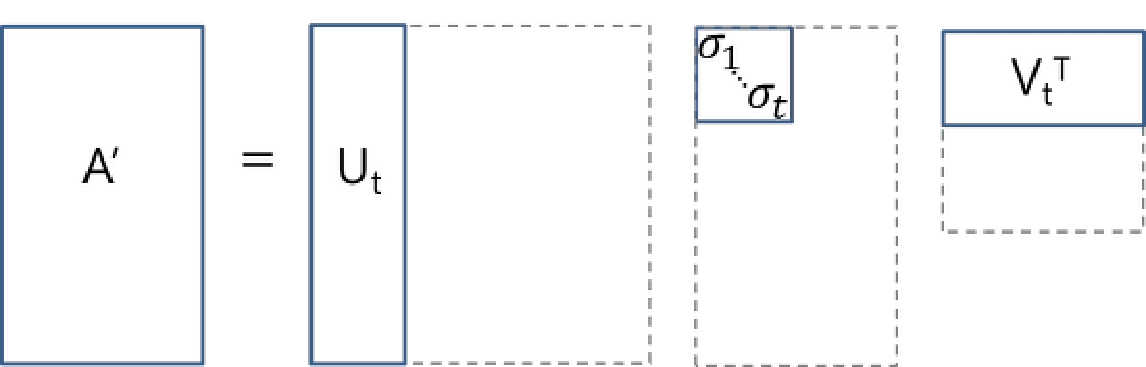
\includegraphics[width=0.70\textwidth]{lsa.pdf}
    \caption{LSA使用SVD分解原理图}
    \label{fig:lsa}
\end{figure}

概率隐语义分析(Probability Latent Semantic Analysis,PLSA)\citep{Hofmann1999PLSA}与LSA基础思想一致,都是希望找出词隐含的语义。二者区别在于LSA缺乏严谨的数理统计基础,且没有明确的物理解释,使用SVD分解操作。而PLSA使用概率模型,具有更明确的物理意义,并且使用期望最大化算法(Expectation-Maximization,EM)来学习模型参数。PLSA在文档和词之间构造隐含主题。PLSA认为一篇文档通常由多个隐含主题构成,而每个隐含主题由多个与该主题最相关的词来描述。即文档以一定的概率选择隐含主题,隐含主题以一定的概率选择词。PLSA建模思想简单,针对观察到的变量使用似然函数建模。建模中暴露出隐含变量,难以直接使用极大似然估计,所以使用EM算法求解。PLSA原理如图\ref{fig:plsa}所示。
\begin{figure}[!htbp]
    \centering
    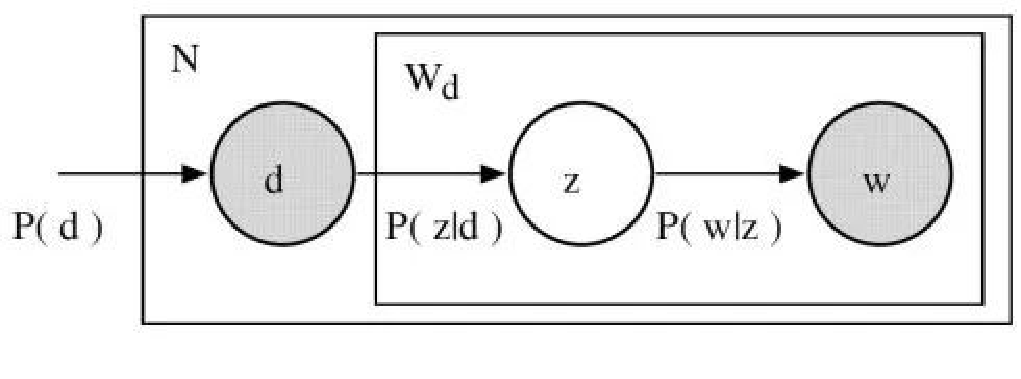
\includegraphics[width=0.70\textwidth]{plsa.pdf}
    \caption{PLSA原理图}
    \label{fig:plsa}
\end{figure}

隐狄利克雷分布(Latent Dirichlet Allocation,LDA)\citep{blei-2003-LDA}是PLSA的泛化版本。LDA认为文档到主题服从多项式分布,主题到词也服从多项式分布。LDA将PLSA中的参数变成随机变量,并且加入狄利克雷先验得到贝叶斯模型。使用狄利克雷先验主要是利用了狄利克雷分布和多项式分布的共轭性,方便计算。当将LDA的超参数设为特定值时,就特化成PLSA。LDA与PLSA的本质区别是估计参数的思想不同,PLSA使用频率派的思想,LDA使用贝叶斯派的思想。LDA的原理如图\ref{fig:lda}所示。其中$\alpha$和$\beta$是两个不同的狄利克雷分布的参数,分别用来生成隐含主题的分布参数$\theta$和词的分布参数$\varphi$。$z$和$w$分别是从各自分布中选出的隐含主题和特定的单词。
\begin{figure}[!htbp]
    \centering
    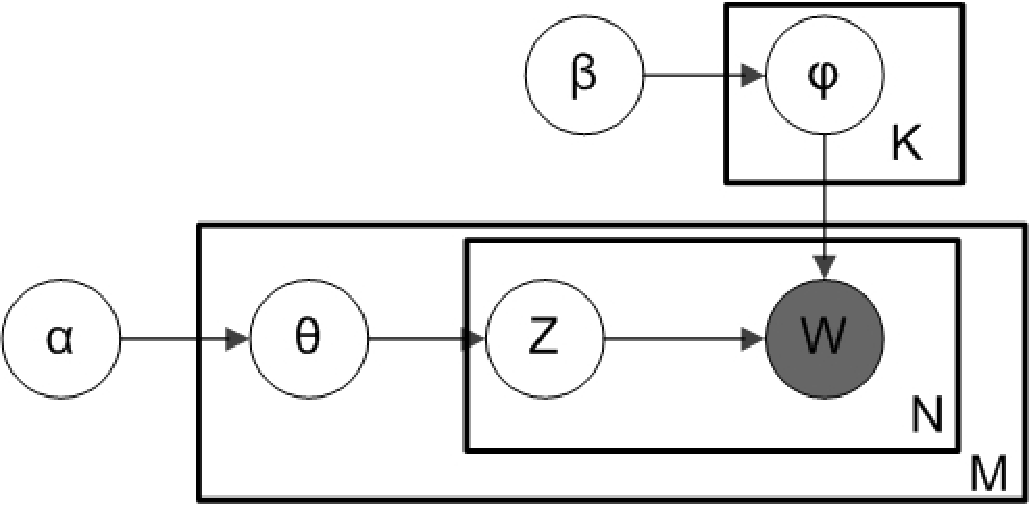
\includegraphics[width=0.70\textwidth]{lda.pdf}
    \caption{LDA原理图}
    \label{fig:lda}
\end{figure}

除了上述三种主题模型外,还有层级狄利克雷过程(Hierarchical Dirichlet Processes,HDP)\citep{the2006hierarchical}及各种主题模型的变种。这些主题模型通常在长文本上效果较好。然而,在短文本的网络数据中的效果却非常差。这是因为短文本导致词共现较少,而这些主题模型严重依赖于词的共现性,所以主题模型不能直接用来对稀疏的网络数据进行话题检测。

同时,网络数据不再是单一模态的文本数据,更多的是诸如文本、图片、音频、视频等多模态的异构数据的融合。针对多模态数据,许多文献将网络话题检测任务当做基于多模态数据的聚类任务。有两个主流的研究路线。一个是基于多模态的方法\citep{blei-lafferty-2007-correlatedtopicmodel,putthividhy-2010-multimodalLDA},另一个是基于相似度图的方法\cite{papadopoulos-2011-cluster}。

在基于多模态方法中,网络话题检测主要有两种研究方法:第一个研究方法是在多个模态的数据上进行聚类算法的研究。这种方法主要是将单模态的方法扩展到多模态数据。比如由LDA演变而来的多模态的LDA\citep{putthividhy-2010-multimodalLDA}提出从图片及其标签来检测话题。第二个研究方法是将多个模态的信息进行融合,再在融合后的信息上进行研究\cite{jia2011learning,Oh2014multimedia}。这种方法通过融合不同模态的信息以获得更大的信息量,再通过聚类算法检测网络话题。

在基于相似度图的方法中,多模态数据被融合进图中的边,然后将图中的顶点聚类成不同的话题。例如,Wu等人在论文\citep{wu-2007-crosslingual}中通过融合来自近似重复帧(Nearly-Duplicated Keyframes,NDKs)和演讲手稿的相似度来检测新闻视频中的话题。与基于多模态的主题模型相比,基于相似度图的方法可以很容易地扩展到其他算法\citep{cao-2011-tracking,aiello-2013-sensing,papadopoulos-2011-cluster}。

在聚类过程时,当前比较流行的聚类定义是计算话题内部的相似度。例如,Pang等人在\citep{pang-2013-unsupervised}使用相似度图中的最大团当作话题。Wang等人在\citep{wang2008automatic}中使用基于成对相似度的凝聚类算法来发现新闻中的话题。Cao等人在\citep{cao-2011-tracking}中通过k-means聚类算法在视频及其标签融合的相似度图上进行聚类。Zhang等人在\citep{zhang2013cross}中提出使用图转移(Graph Shift,GS)\citep{liu2010graphshift}算法来寻找密集子图作为话题。这些类内相似度方法通常只能发现一小部分热点话题,导致召回率相当低。因为简单的类内相似度方法并不能很好地解决当前稀疏并且充满噪声的网络数据。

与单纯计算类内相似度相反,一些方法采用了高级的聚类算法。论文\citep{xu2003document}使用非负矩阵分解算法(Nonnegative Matrix Factorization,NMF)来进行话题检测。与在文档上使用谱聚类算法相比,性能更好。然而这些高级方法在面对网络数据这种大规模的数据集时显得有些力不从心。无论是谱聚类算法还是非负矩阵分解算法,针对大规模数据时的复杂度非常高,导致网络话题检测效率很差。

实际上,由于网络数据的稀疏性以及高噪性,导致网络话题并不等同于聚类\citep{cao-2011-tracking}。因此,Pang等人在论文\cite{pang-2013-unsupervised}中将网络话题检测问题转化为无监督的排序问题,并提出PD算法来对话题权重进行计算。PD算法通过已有的聚类算法\citep{yang2012clustering,li2007noise}来获得过完备的话题集合,然后计算话题兴趣度,最后通过对话题的兴趣度进行排序来检测热点话题。然而,对PD算法来说,在大规模网络数据中产生过完备话题是一个非常耗时的过程\citep{pang-2013-unsupervised,pang-tao-2016-lpd}。

尽管许多方法提出解决大规模数据的话题检测问题,但是,据我们目前所知,只有一些方法试图通过并行LDA\citep{chen-2015-WarpLDA,wang-2009-PLDA,Liu-2011-PLDA+}来解决。正如在\citep{pang-2013-unsupervised,pang-tao-2016-lpd}所讨论的,LDA假设每个网页至少属于一个话题。然而,就网络数据而言,几乎有95\%的网页不能组织成话题。因此,并行化的LDA不能去除网络数据中所包含的大量的噪声网页。



\section{解决方案}

本论文研究面向大规模网络数据的话题检测。主要解决两方面问题,一个是针对网络话题的特点产生的问题,另一个是针对网络数据特点产生的问题。这些问题统计如下:
\begin{enumerate}
	\item[1] 针对网络话题特点而产生的问题:
		\begin{enumerate}
			\item[(1)] 话题大小不确定性问题:主要由于每个人对话题的认识不同,导致话题大小的界定有差异;
			\item[(2)] 话题数量不确定性问题:同样是由于每个人对话题的认识不同,导致话题之间的界限不明确;
		\end{enumerate}
	\item[2] 针对网络数据特点而产生的问题:
		\begin{enumerate}
			\item[(1)] 低质量的特征表示问题:主要是由于短文本的网络数据导致稀疏的特征表示;
			\item[(2)] 大量的噪声数据问题:主要是由于网络数据受到较少约束导致的大量错误、冗余、无关的数据。
			\item[(3)] 大规模的数据问题:主要是由于人能够便捷地网络上随意创作而带来的网络数据的爆炸式增长。
		\end{enumerate}
\end{enumerate}

基于上述问题,我们调研了目前国内外关于话题检测的相关文献。发现当前解决网络话题检测问题的比较优秀的方法是Pang等人在论文\citep{pang-2013-unsupervised}中提出的基于无监督排序的网络话题检测算法。该算法将网络话题检测问题转换为无监督的多粒度话题排序问题,从而避免了确定话题数量和大小的问题。该算法主要分为三个阶段:构造相似度图、生成多粒度话题、通过无监督排序确定真实话题。其中在构造相似度图时只保留最相近的$knn$个网页,从而达到过滤噪声的目的。然后在多级相似度图上使用最大团算法(Maximum Clique, MC)生成多粒度话题。最后在相似度图上基于泊松分布实现泊松去卷积算法来计算话题权重。虽然该论文最终比其他传统方法取得更好的结果,然而没有解决低质量的特征表示问题和大规模数据问题。

随后,Pang等人在\citep{pang-tao-2016-lpd}中通过融合多模态信息来提高特征质量,并且采用了更高级的聚类算法——基于随机游走的非负矩阵分解算法(Nonnegative Matrix Factorization Using Random Walk, NMFR)来生成多粒度话题。然而NMFR算法虽然能够提高聚类质量,但是同时也带来很高的时间复杂度。所以该论文还是没有解决大规模网络数据问题。

因此,本论文试图改进Pang等人提出的基于无监督排序的网络话题检测算法,以便更好地处理大规模网络数据。也就是说,本论文的最终目的是解决该算法的可扩展性问题。因此,我们主要针对该算法的两个部分进行改进。

\subsection{生成多粒度话题}

Pang等人使用过MC算法和NMFR算法在多级相似度图上生成多粒度话题。然而这两个算法都是非常耗时的算法,无法高效地处理大规模网络数据。跟传统方法一样,MC算法采用了一个看似合理的假设:相同话题内的网页之间的类内相似度应该大于话题内的网页和噪声网页之间的类间相似度。然而,由于低质量的特征表示以及语义鸿沟等问题导致这个假设站不住脚。与此同时,我们在研究真实话题在相似度空间的统计模式后,发现网络话题的组织模式与L\'evy Walks存在统计意义上的相似性\citep{perkins2014ascaling}。具体的,如果我们将网页间的相似度类比为L\'evy Walks中的步长,那么一个话题内的相似度分布符合重尾分布,而重尾分布被用来定性L\'evy Walks中的步长。

L\'evy Walks\citep{viswanathan2001levy,rhee2011levywalk}是随机游走模型中的一种。其中的步长服从某种重尾的概率分布。L\'evy Walks中的$flight$定义为一个质点从一个位置无偏移地移动另一个位置的步长。如图\ref{fig:levywalks}展示了L\'evy Walks中的$fligh$分别从柯西分布和正太分布中采样1000次的结果。直观上讲,L\'evy Walks包含许多较短的$flight$和一些额外较长的$flight$。因此,L\'evy Walks可以被用来描述诸如蜘蛛猴这样觅食动物的迁徙模式\citep{viswanathan2001levy}。同时,L\'evy Walks提供了一种更为有效的访问结点的方法\citep{li2010towards}。L\'evy Walks的另一个重要应用是在一个网络中路由\citep{perkins2014ascaling}。
\begin{figure}[!htbp]
    \centering
    \begin{subfigure}[b]{0.5\textwidth}
      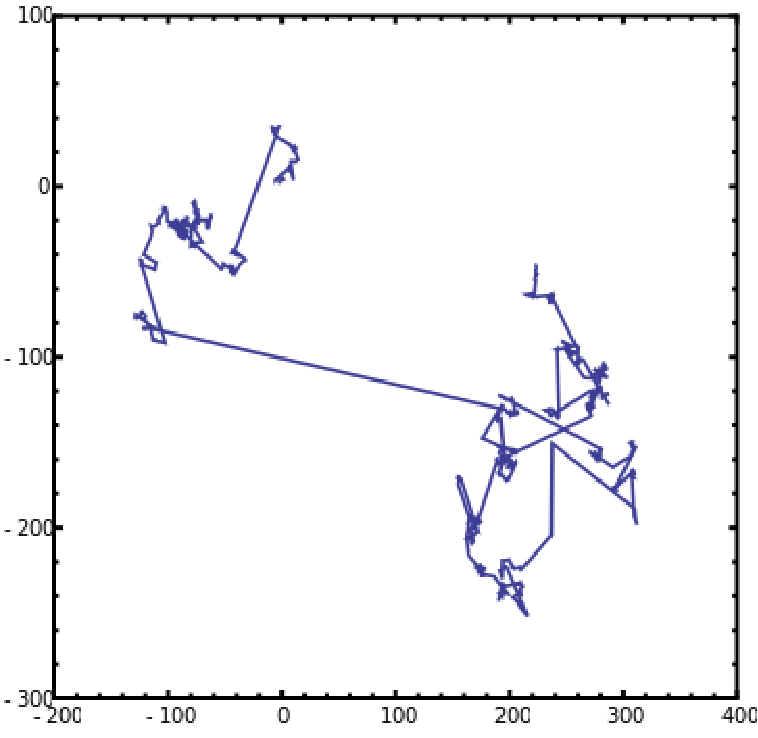
\includegraphics[width=\textwidth,height=0.9\textwidth]{CauchyDistribution}
      \caption{步长服从柯西分布}
      \label{fig:CauchyDistribution}
    \end{subfigure}%
    \begin{subfigure}[b]{0.5\textwidth}
      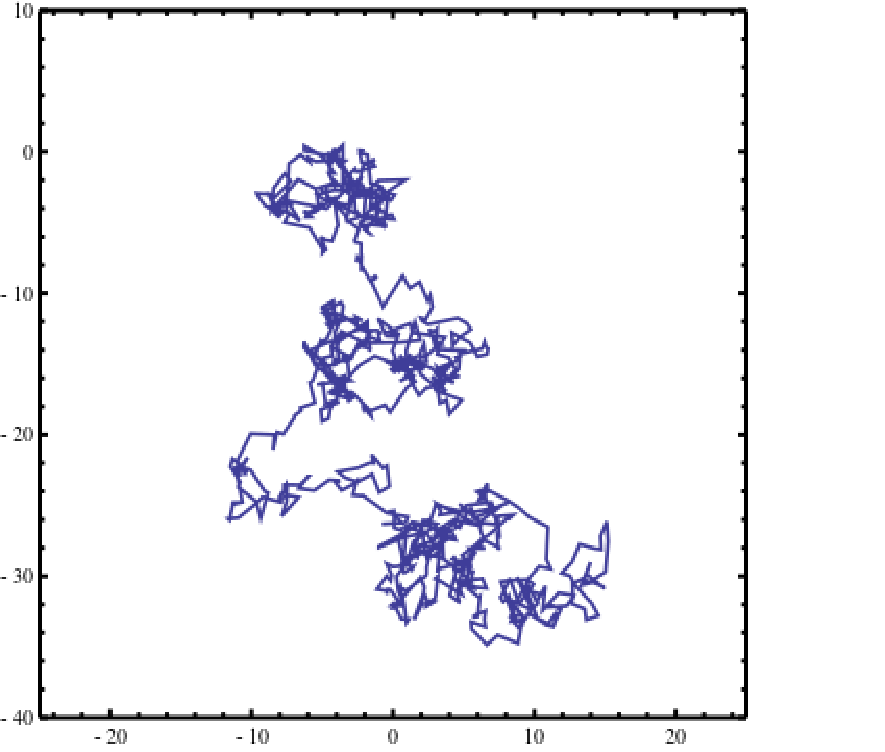
\includegraphics[width=\textwidth,height=0.9\textwidth]{BrownianMotion}
      \caption{步长服从正太分布}
      \label{fig:BrownianMotion}
    \end{subfigure}
    \caption{1000步L\'evy flight在二维坐标上的例子}
    \label{fig:levywalks}
\end{figure}

当L\'evy Walks被用来组织网络话题时,关键问题变成:1)如何在未知分布参数情况下模拟L\'evy Walks中额外较长的步长;2)如何确定所需步长的数量来组织话题;3)如何快速处理大规模的网络数据。基于上述3个问题,我们提出提出了下面对应解决方案:
\begin{enumerate}
	\item[(1)] 我们采用了一种基于种子话题的网页多分配算法来模拟相似度空间中的L\'evy Walks,优雅地避免了确定未知参数的麻烦;
	\item[(2)] 我们采用了层级阈值的方法来截断话题的生长,从而产生一系列过完备的话题,保证了话题的召回率;
	\item[(3)] 我们提出的网页多分配算法只需要进行简单的计算和分配,是一种无模型并且无需复杂参数优化的网络话题快速生成算法,从而向大规模网络数据的处理迈进了一步。
\end{enumerate}

据我们所知,本论文是第一个发现L\'evy Walks和网络话题在相似度空间上具有相似性。并且呈现了一系列完整的实验来证明这个发现对于网络话题检测的好处。我们提出的方法在计算上很简单但是效果非常好。仅仅通过简单的选择种子网页并且将网页分配到由种子网页生成的多个最相似的话题,无需进一步的参数调整等操作,我们找到一个新的组织网络话题的方式。并且在话题生成质量上比得上当前最好的方法,同时在话题生成效率上大大超过当前最好的方法。



\subsection{无监督排序}

Pang等人在论文\citep{pang-2013-unsupervised}中基于泊松分布假设提出泊松去卷积算法(Poisson Deconvolution,PD)。PD算法通过扩散网页之间的相似度来对每个话题分配一个权重。虽然相似度图可以通过在线$k$近邻图($k$-Nearest Neighborhood Graph, $k$N$^2$G)\citep{debatty-2016-fastonlineknn}构建,同时也可以通过稀疏矩阵的方式来高效的存储。但是,一个严重的问题是PD算法无法高效地处理大规模的网络数据。因为PD算法在每一轮必须使用所有数据在内存中重构一个$N\times N$的浮点型矩阵,其中$N$是网页数量。

那么我们是否可以在每一轮迭代更新时只使用一小部分数据来更新呢?一个简单但是有效的方法是随机优化\citep{hannah-2015-Stochastic}。这类方法至少能带来两个好处:1)减少物理内存的要求;2)避免一个$N\times N$规模的相似度图的重构。例如随机梯度下降(Stochastic Gradient Descent,SGD)及其变种\citep{Roux-2012-sgd-exponential,johnson-2013-sgd-accelerating,Nitanda-2014-sgd-proximal}由于优秀的效果和效率,已经广泛应用于机器学习。然而,通过EM算法优化的PD算法需要保持一个和相似度图同等规模的隐变量,并且PD算法的目标函数在每轮迭代时随着期望变化而变化。所以SGD算法并不能够解决基于EM算法优化的PD算法。

优化最小化原则(Majorization Minimization,MM)\citep{lange-2000-optimization}是EM算法的泛化版本。取目标函数的上界作为代理函数,然后迭代地最小化代理函数。许多方法可以用MM原则来解释,例如变分贝叶斯(Variational Bayes)
\citep{Wainwright-2008-variational-bayes}和近端算法(Proximal Algorithm)\citep{beck-2009-fastshrinkage}。随后,论文\citep{mairal-2013-SMM}提出随机优化最小化原则(Stochastic Majorization Minimization,SMM)使得MM具有可扩展性。

受到SMM的启发,我们提出随机泊松去卷积算法(Stochastic Poisson Deconvolution,SPD)来对PD算法进行可扩展性改造。SPD迭代地更新目标函数上界构成的代理函数。最终的SPD算法不仅只需要存储一小部分采样边,而且极大地加速了算法的收敛速度。

据我们所知,本文是第一个致力于解决PD算法的可扩展性问题,并将基于代理函数的优化原则用于PD算法中。提出的SPD算法不仅概念上简单,而且非常有效。
\chapter{网络话题的快速生成}\label{chap:topicGeneration}
\section{引言}

随着社交媒体的快速发展,越来越多的用户通过社交媒体来获取信息和分享观点。由此产生了海量的用户生成式数据,使得用户难以从中快速获取热点话题及感兴趣的话题。话题是某个种子事件及其相关报道的集合。网络话题检测任务自动地将网络数据组织成更多有意义的热门话题。从本质上来讲,网络话题检测就像从大海里捞针,类比从大量的网络数据中找到一小部分感兴趣数据并将其组织成热门事件。

传统的话题检测任务致力于将每个新闻文章分配到至少一个话题中。而这些经过专业编辑的新闻文章数据与网络数据存在极大的差异:由于社交媒体对所发布内容的约束较少,所以来自社交媒体的网络数据更加简短、稀疏并且充满噪声;在大量网页中,只有一小部分的网页能够被组织成热点话题。因此网络话题检测不仅面临着低效的特征表达还需要处理大量的噪声网页。

网络话题检测的关键问题是如何在海量噪声网页存在的前提下组织热点话题。一个直观的方法是在噪声网页存在的情况下去聚类网络话题。然而海量的噪声网页使得传统方法不再适用。为了移除大量噪声网页带来的不利影响,传统的方法采用了一种看似合理的假设,即在相同话题下的任意两个网页之间的相似度应该大于该话题中的网页和噪声网页之间的相似度。然而,这个假设也很难站得住脚,主要存在如下两个挑战:

\begin{enumerate}
\renewcommand{\labelenumi}{\theenumi)}
    \item 稀疏和充满噪声的网络数据导致低效的特征:用户生成式数据几乎没有约束,所以传统的适用于长文本的TF-IDF特征不足以高效表达社交媒体上稀疏的、充满噪声的网络数据。
    \item 低阶特征和高阶语义间存在的语义鸿沟:低阶的特征难以准确地表达高阶语义间的关系。所以网页之间更大的相似度值并不意味着这两个网页在语义上更加相似。
\end{enumerate}

在低效的特征表示以及海量噪声存在的前提下,我们寻找一种无关模型、无关优化的的方法来生成网络话题。首先是因为网络话题的结构和内容差异性很大,一个无模型的方法能拥有好的生成话题能力;其次,为了避免高复杂度的优化措施,一个无需优化的方法能够更好地处理大规模数据问题;然后,我们避免去处理短文本如何编码生成高效的特征表示这样一个开放性问题;最后网络话题面临着海量噪声。

我们研究了网络话题在相似度空间上的统计模式,发现同一个话题下的所有网页之间的相似度与L\'{e}vy Walks存在统计意义上的相似性。具体地,我们将网页之间的相似度类比为L\'{e}vy Walks中的步长,那么一个热点话题中的所有相似度分布大致服从重尾分布,而这重尾分布又是L\'{e}vy Walks中步长的特性。L\'{e}vy Walks是一种随机游走模型,其步长服从重尾概率分布。一次移动定义为一个质点从一个位置无偏移的移动到另一个位置的步长。直观上讲,L\'{e}vy Walks包含许多短步长的移动和一些逃脱短步长控制的额外较长步长的移动。因此,L\'{e}vy Walks可以用来很好地描述觅食动物的迁徙模式。

当L\'{e}vy Walks被用来组织网络话题,关键问题变成如下几点:
\begin{enumerate}
\renewcommand{\labelenumi}{\theenumi)}
    \item 如何在未知参数下模拟L\'{e}vy Walks中额外长的步长。
    \item 如何确定话题所需要的步长个数即网页个数。
    \item 在组织话题的时候选择这个步长是否能带来好处。
\end{enumerate}
基于上述三个问题,我们提出以下解决方案:
\begin{enumerate}
\renewcommand{\labelenumi}{\theenumi)}
    \item 提出基于L\'{e}vy Walks的话题生成算法(L\'{e}vy Walks-based Topic Generation,LWTG),该方法通过模拟L\'{e}vy Walks的特性,采用基于种子网页的多分配策略,优雅地避免了不同L\'{e}vy Walks需要不同参数的麻烦。简单的同时速度也很快。
    \item 提出多阈值方法来截断网络话题的生长,这会带来一系列过完备话题,从而提高话题的召回率。
    \item 至于话题召回准确率是由后续的排序算法来保证的。
\end{enumerate}

\begin{figure}[!htbp]
    \centering
    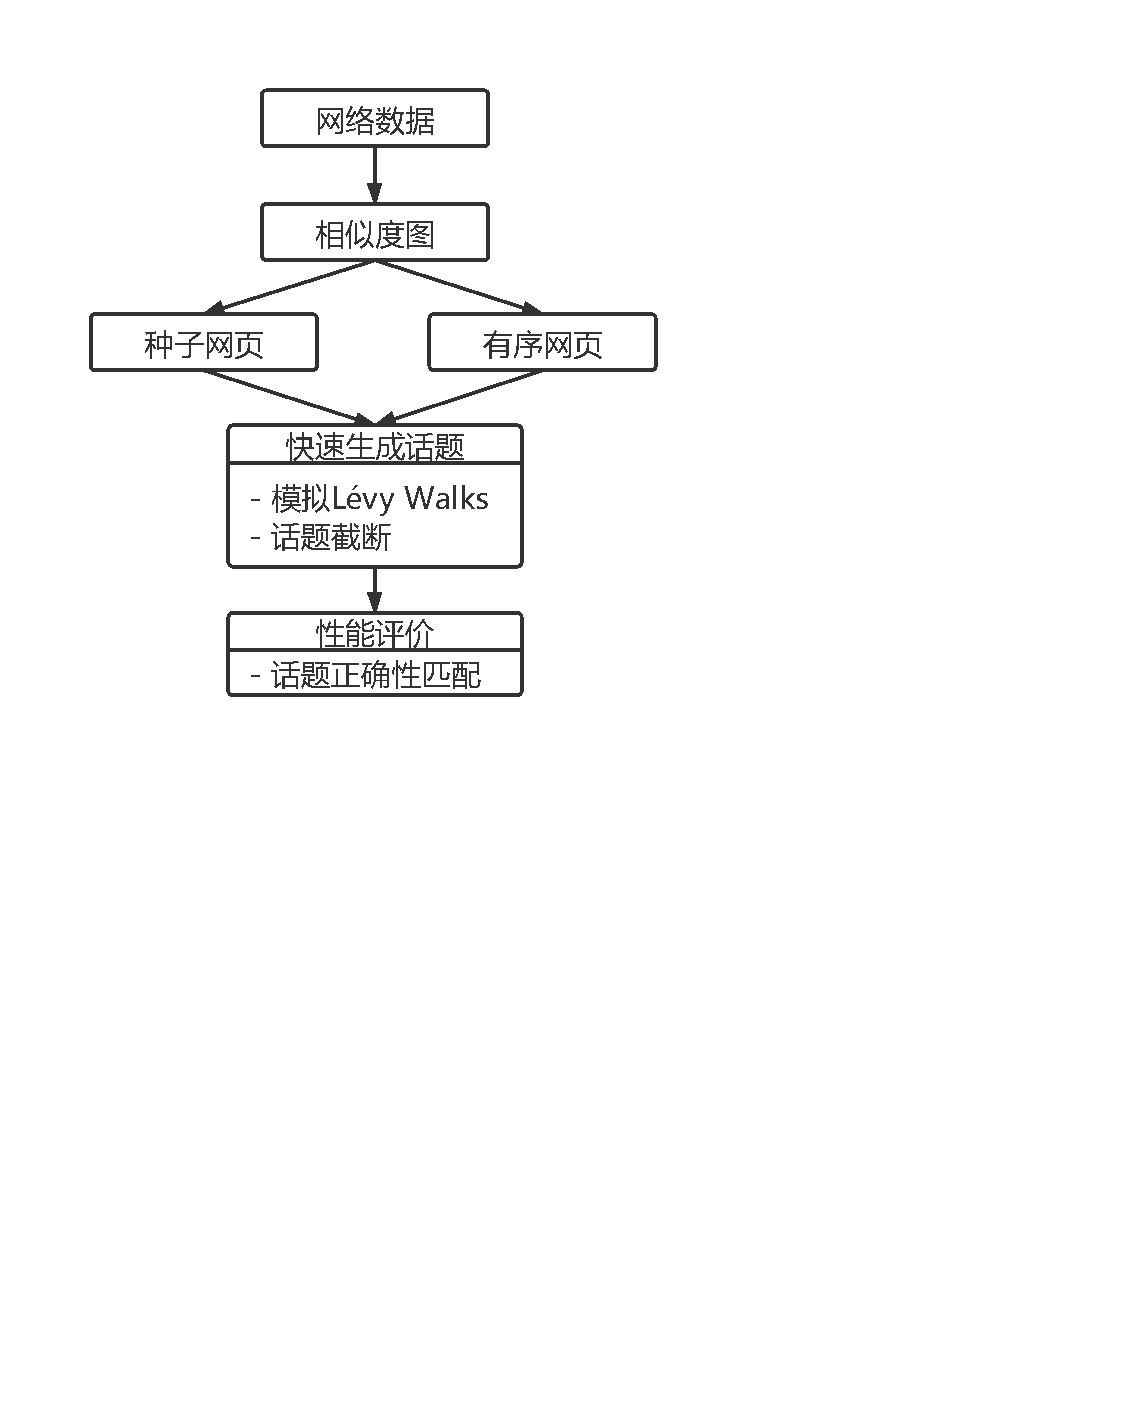
\includegraphics[width=0.50\textwidth]{topic_generation_process.pdf}
    \caption{通过模拟L\'evy Walks来快速生成网络话题的流程图}
    \label{fig:topic_generation_process}
\end{figure}

本论文是第一个发现网络话题检测在相似度空间上和L\'{e}vy Walks具有相似的特点,并且进行了一系列实验来阐述这个发现所带来的好处。我们提出的LWTG方法不仅简单快速,而且能够进一步提高话题检测的召回率。通过简单地对网页进行分配,无需参数优化,我们找到了一种新的组织网络话题的方法。我们的方法在网络话题检测效率方面已经远超当前最好的方法,而且在话题检测召回率方面也能够赶上甚至超越当前最好的方法。算法框架如图\ref{fig:topic_generation_process}所示。

\section{相似度图的构建}

本章的研究重点是网络话题的生成,因此,为了减少其他因素的影响,我们忽略网络数据的多模态性和时间戳、链接等其他信息,只使用纯文本信息。所以每个网页就是一个文本字符串。对于给定的网络数据集,包含一系列的网页$W=\{w_1,...,w_N\}$,我们对其进行处理,生成一个$knn$近邻的相似度图$G=(V,E,A)$。其中顶点集$V$对应网页集合,仿射矩阵$A$对应截断后任意两个网页之间的相似度,边集$E$对应任意两个网页之间的非$0$边[xx]。具体处理如下。

首先,我们对网页的文本字符串进行分词,然后使用词袋模型[xx]对网页文本进行基本的统计和表示,再用TF-IDF特征值表示每个词的权重,这样每个网页就可以用一个特征向量$x_i\in \mathbb{R}^M(i=1,...,N)$表示。其中M是表示词典大小,N表示网络数据集中网页的数量。对于TF-IDF特征,TF表示词频,IDF表示逆文档频率。一个词在文档中出现的频率越高,其词频值越大,相应TF-IDF值就越大。与此同时,一个词如果出现在越多的文档中,则其逆文档频率值越低,相应TF-IDF特征值就越低。逆文档频率降低那些高频出现但是较没有判别意义的词的权重。比如:‘我’、‘那’这种指示代词几乎没有判别能力,虽然它们的词频值很大,但是它们的逆文档频率值很低,进而使得TF-IDF值很低。虽然还可以使用更高级的特征,但是语义鸿沟问题仍然存在,而且使用TF-IDF特征足够简单,能够带来更快的处理速度。

然后,基于得到的每个网页的特征向量,我们可以通过余弦距离来度量两个网页之间的相似度大小。在公式\ref{eq:cosinedistance}中,$S_{ij}$表示两个网页之间的相似度,$x_i$和$x_j$表示两个网页的特征向量:
\begin{equation}\label{eq:cosinedistance}
    S_{ij} = \frac{x_i\cdot x_j}{|x_i||x_j|}
\end{equation}

最后,得到相似度图后,在每个网页中,保留与其语义最相近的$knn$个网页关系,删除其他网页关系。这里假设两个网页之间相似度越高则语义越相近。这样做能够过滤掉大量网页之间的噪声干扰,即不相关的噪声网页。网络数据集中的噪声网页越多,$knn$应该选择更低的值。在公式\ref{eq:knn}中$KNN(w_i)$表示与网页$w_i$语义最相近的$knn$个网页集合。同时,我们使用公式\ref{eq:filtergraph}将两个网页之间低于某个阈值的相似度置为$0$,因为我们认为过低的相似度表示这两个网页在语义上已经没有关联关系了。这进一步过滤了噪声网页。
\begin{equation}\label{eq:knn}
S_{ij} = 
\begin{cases}
0, &  w_j \notin KNN(w_i) \\
S_{ij}, & w_j \in KNN(w_i)
\end{cases}
\end{equation}

\begin{equation}\label{eq:filtergraph}
S_{ij} = 
\begin{cases}
0, & S_{ij} < \epsilon \\
a_{ij}, & S_{ij} \geq \epsilon
\end{cases}
\end{equation}


\section{网络话题的L\'{e}vy Walks特性}
一个网络话题由未知数量的网页构成,在相似度空间上表示为一系列边$e_{ij}$经过仿射后的相似度$a_{ij}$,其中网页$x_i$和$x_j$属于该话题。话题的相似度空间包含两种相似度:1)话题内部相似度边:同个话题内部两个网页之间的相似度;2)话题之间相似度边:两个不在同个话题内的网页之间的相似度。

\begin{figure}[!htbp]
    \centering
    \begin{subfigure}[b]{0.24\textwidth}
      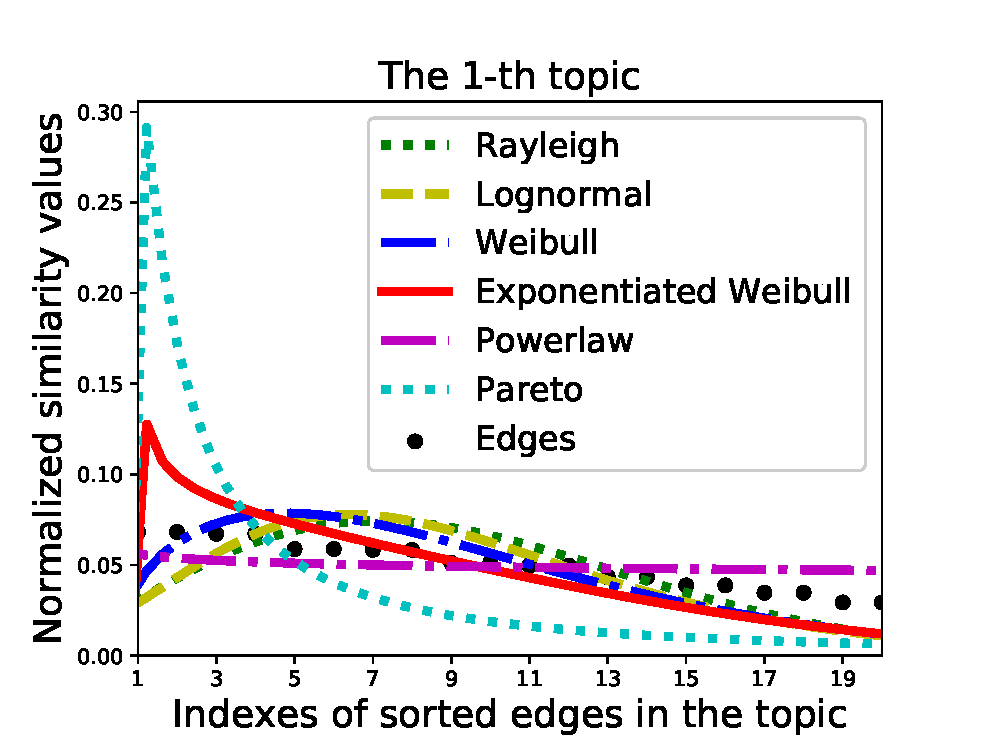
\includegraphics[width=\textwidth]{fit_distribution_topic_1}
      \caption{}
      \label{fig:fitdistribution_t1}
    \end{subfigure}%
    % ~% add desired spacing
    \begin{subfigure}[b]{0.24\textwidth}
      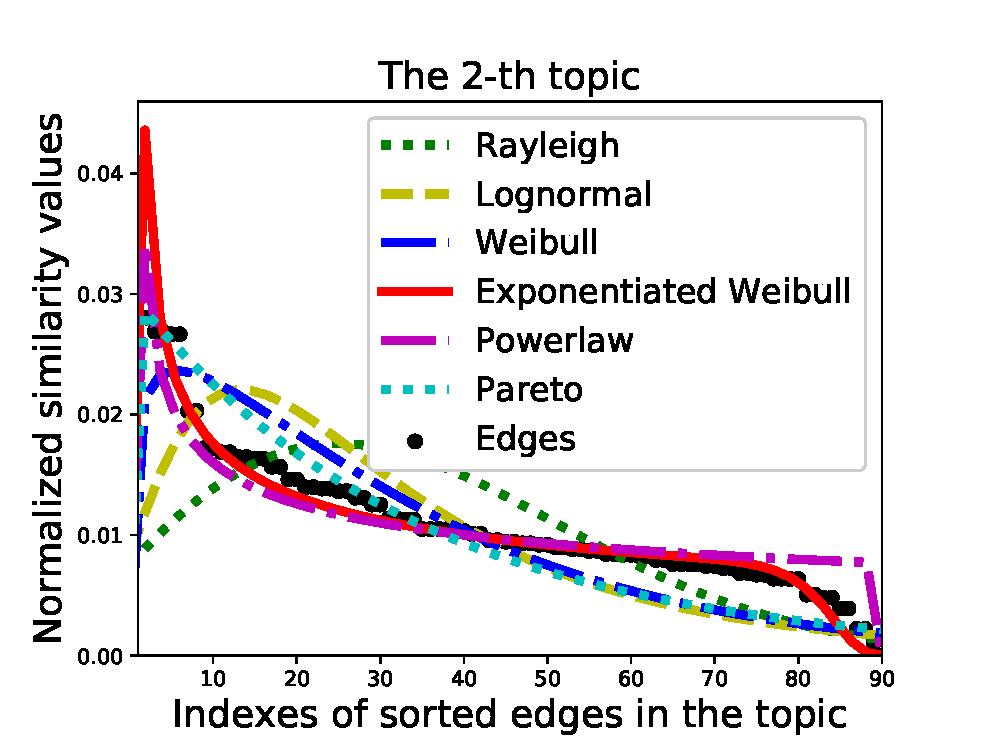
\includegraphics[width=\textwidth]{fit_distribution_topic_2}
      \caption{}
      \label{fig:fitdistribution_t2}
    \end{subfigure}
    % \\% line break
    \begin{subfigure}[b]{0.24\textwidth}
      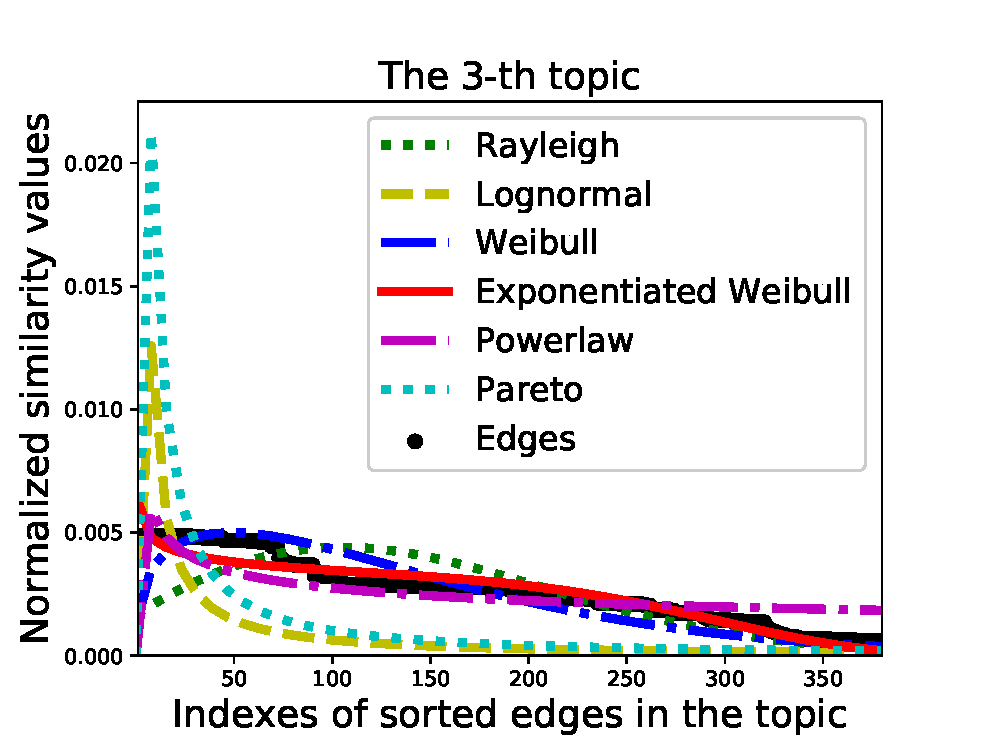
\includegraphics[width=\textwidth]{fit_distribution_topic_3}
      \caption{}
      \label{fig:fitdistribution_t3}
    \end{subfigure}%
    % ~% add desired spacing
    \begin{subfigure}[b]{0.24\textwidth}
      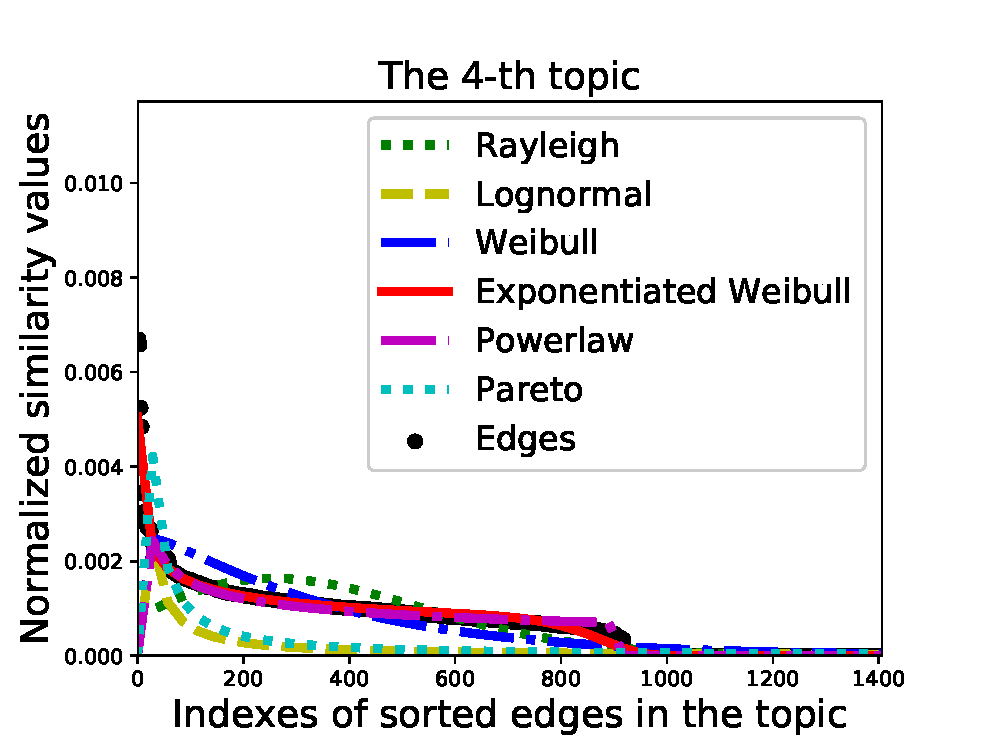
\includegraphics[width=\textwidth]{fit_distribution_topic_4}
      \caption{}
      \label{fig:fitdistribution_t4}
    \end{subfigure}
    \caption{第1、2、3、4个话题分别最拟合指数韦伯分布,幂次分布,指数韦伯分布,幂次分布。}
    \label{fig:fitdistribution}
\end{figure}

\begin{figure}[!htbp]
    \centering
    \begin{subfigure}[b]{0.24\textwidth}
      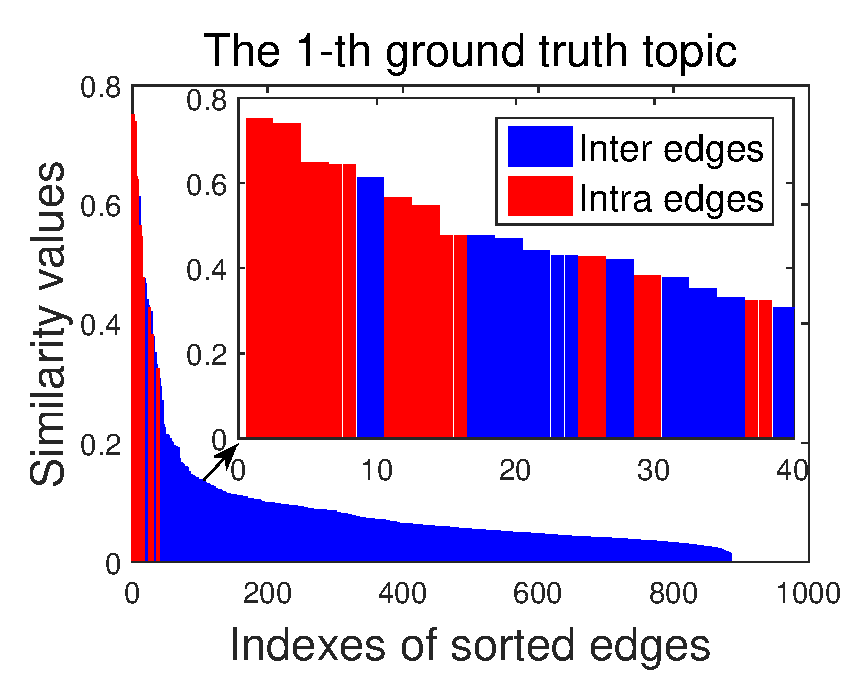
\includegraphics[width=\textwidth]{barGraph_topic_1}
      \caption{}
      \label{fig:barGraph_t1}
    \end{subfigure}%
    % ~% add desired spacing
    \begin{subfigure}[b]{0.24\textwidth}
      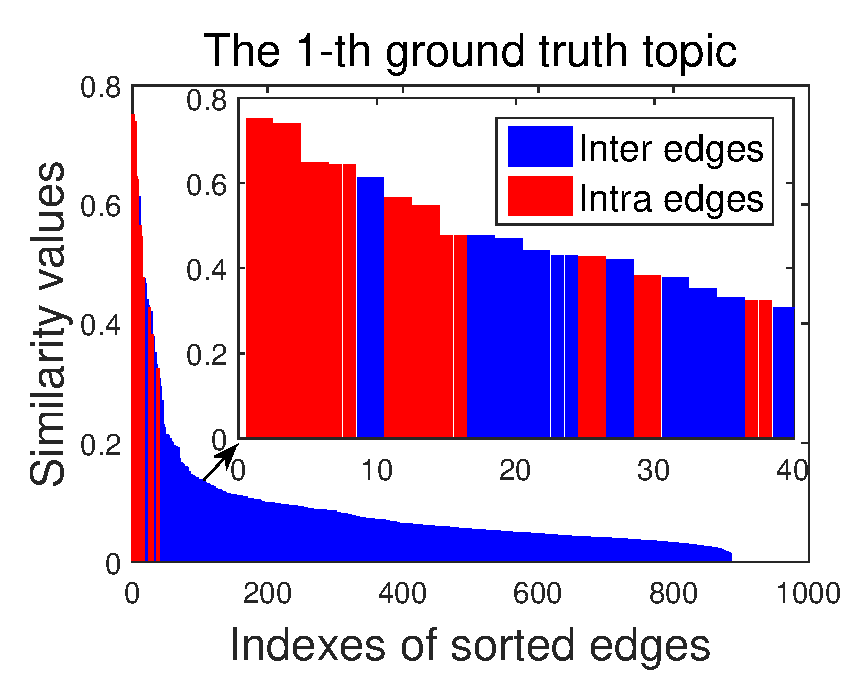
\includegraphics[width=\textwidth]{barGraph_topic_1}
      \caption{}
      \label{fig:barGraph_t2}
    \end{subfigure}
    % \\% line break
    \begin{subfigure}[b]{0.24\textwidth}
      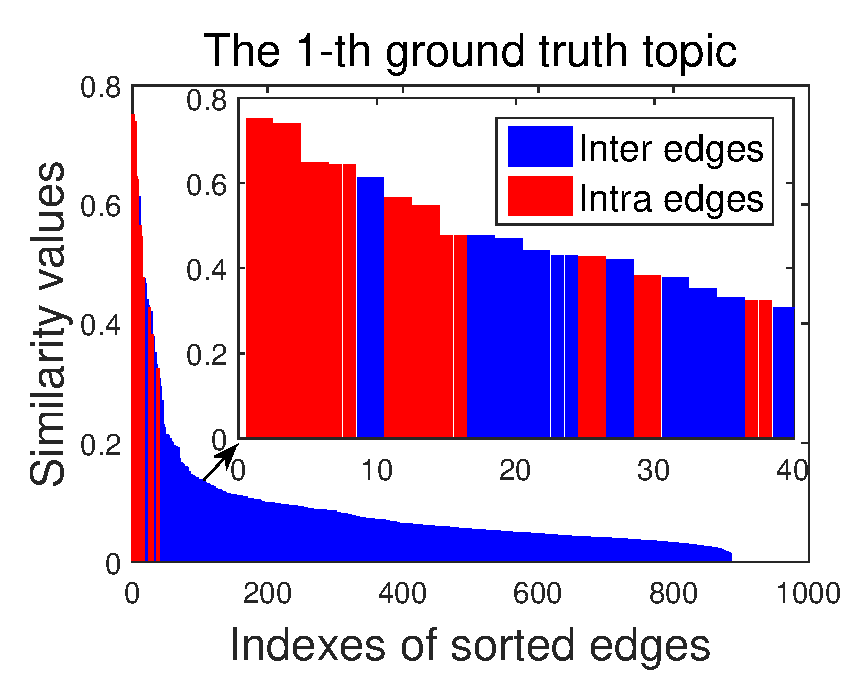
\includegraphics[width=\textwidth]{barGraph_topic_1}
      \caption{}
      \label{fig:barGraph_t3}
    \end{subfigure}%
    % ~% add desired spacing
    \begin{subfigure}[b]{0.24\textwidth}
      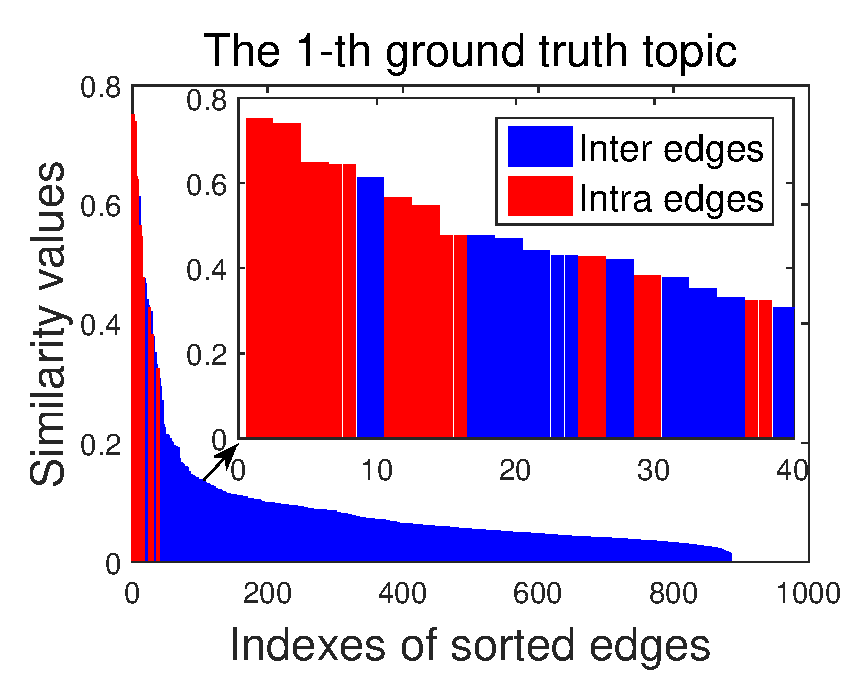
\includegraphics[width=\textwidth]{barGraph_topic_1}
      \caption{}
      \label{fig:barGraph_t4}
    \end{subfigure}
    \caption{已排序边的分布情况,包含话题内部的边和话题之间的边。}
    \label{fig:barGraph}
\end{figure}

\begin{table}[!htbp]
    \caption{常见的重尾分布函数。}
    \label{tab:PDF}
    \centering
    % \footnotesize% fontsize
    \setlength{\tabcolsep}{4pt}% column separation
    \renewcommand{\arraystretch}{1.2}%row space 
    \begin{tabular}{|c|c|}
        \hline
        分布函数 & 概率密度函数\\
        \hline\hline
        指数韦伯分布$^1$ & $(1-\exp(-\frac{x}{\lambda})^k)^{\alpha}$\\
        \hline
        锐利分布 & $\frac{x}{\sigma^2}\exp(\frac{-x^2}{2\sigma^2})$\\
        \hline
        韦伯分布$^2$ & $\frac{k}{\lambda}(\frac{x}{\lambda})^{k-1}\exp(-(\frac{x}{\lambda})^k)$\\
        \hline
        对数正态分布 & $\frac{1}{x\sigma\sqrt{2\pi}}\exp(-\frac{\ln(x)-\mu}{2\sigma^2})$\\
        \hline
        幂次分布 & $a(cx)^{-k}$\\
        \hline
        帕累托分布$^3$ & $\frac{\alpha a^{\alpha}}{x^{\alpha+1}}$\\
        \hline
    \end{tabular}\\
    \footnotesize{$^1$ $\alpha \geq 1.$}\\
    \footnotesize{$^2$ $k < 1.$}\\
    \footnotesize{$^3$ $0 < a \leq x$}\\
\end{table}

我们从MCG-WEBV数据集中随机选择四个真实的网络话题来描述网络话题在相似度空间上的模式。对同个话题内部的相似度进行从大到小排序。图\ref{fig:fitdistribution}说明同个话题下的已排序的相似度服从重尾分布。从图\ref{fig:fitdistribution}引出两个问题:
\begin{enumerate}
\renewcommand{\labelenumi}{\theenumi)}
    \item 是否所有的话题服从相同的重尾分布?
    \item 服从相同分布的话题是否拥有相同的分布参数? 
\end{enumerate}

为了解决上述问题,我们使用极大似然估计去将已排序的相似度拟合为已知的分布。例如:指数韦伯分布、锐利分布、韦伯分布、对数正态分布、幂次分布、帕累托分布。表\ref{tab:PDF}列出这些分布的概率密度函数。而且,为了量化最好的分布,我们引入赤池信息准则AIC(Akaike’s Information Criterion)[xxx]:
\begin{equation}\label{eq:AIC}
 AIC = -2log(L(\hat{\theta}|data)) + 2K   
\end{equation}
其中$L(\cdot)$是似然函数,K是参数的数量。由于AIC值容易受样本大小影响,不能被直接用来作为绝对的度量标准。所以,使用下面的转换形式作为每个模型的置信权重:
\begin{equation}\label{eq:AICweight}
    w_i = \frac{exp(-\Delta_i/2)}{\sum_{r=1}^{R}exp(-\Delta_r/2)}
\end{equation}
其中R是分布函数数量。赤池信息权重被认为是分布函数可能性的归一化值。

从图\ref{fig:fitdistribution}到\ref{fig:barGraph},我们可以得到下面观察结果:
\begin{enumerate}
    \item[1)] 同个话题下网页之间的已排序的相似度与L\'{e}vy Walks存在统计意义上的相似特性。图\ref{fig:fitdistribution_t1}、\ref{fig:fitdistribution_t2}、\ref{fig:fitdistribution_t3}、\ref{fig:fitdistribution_t4}表明同个话题内的相似度服从重尾分布。
    \item[2)] 不同的话题服从不同的重尾分布。例如,根据赤池信息权重公式\ref{eq:AICweight},图\ref{fig:fitdistribution_t1}所表示的第一个话题服从指数韦伯分布,而图\ref{fig:fitdistribution_t2}所表示的第二个话题服从幂次分布。
    \item[3)] 热点话题中包含一些额外的边。如图\ref{fig:barGraph}所示,如果话题的相似度按照递减排序,那么由边连接排在较前的网页,并不意味其绝对属于该话题。
\end{enumerate}

如果将相似度类比为网页之间的步长,那么与L\'{e}vy Walks相比,网络话题在相似度空间上有两个统计意义上的相似特性:1)L\'{e}vy Walks和网络话题的步长均服从重尾分布;2)L\'{e}vy Walks和网络话题均包含许多短的步长(高相似度)和一些额外长(低相似度)的步长。至此,这两个相似特性被认为是网络话题的L\'{e}vy Walks特性。

\section{通过模拟L\'{e}vy Walks生成话题}
既然网络话题有L\'{e}vy Walks特性,我们试图从这个特性入手,从海量网络数据中生成话题。一个最简单的办法是根据重尾分布来组织网页进入对应话题。然而,正如之前所言,我们不可能提前训练一个通用的含有重尾分布函数的模型。

通过在相似度空间利用重尾分布的特点,我们认为可以在将网页分配给话题的时候适当添加一定的随机性以模拟L\'{e}vy Walks中额外较长的步长。为此,我们设计了一种通过模拟L\'{e}vy Walks来生成话题的算法(L\'{e}vy Walks-based Topic Generation,LWTG)。LWTG算法的框架如图\ref{fig:LWTG}所示。
\begin{figure}[!htbp]
    \centering
    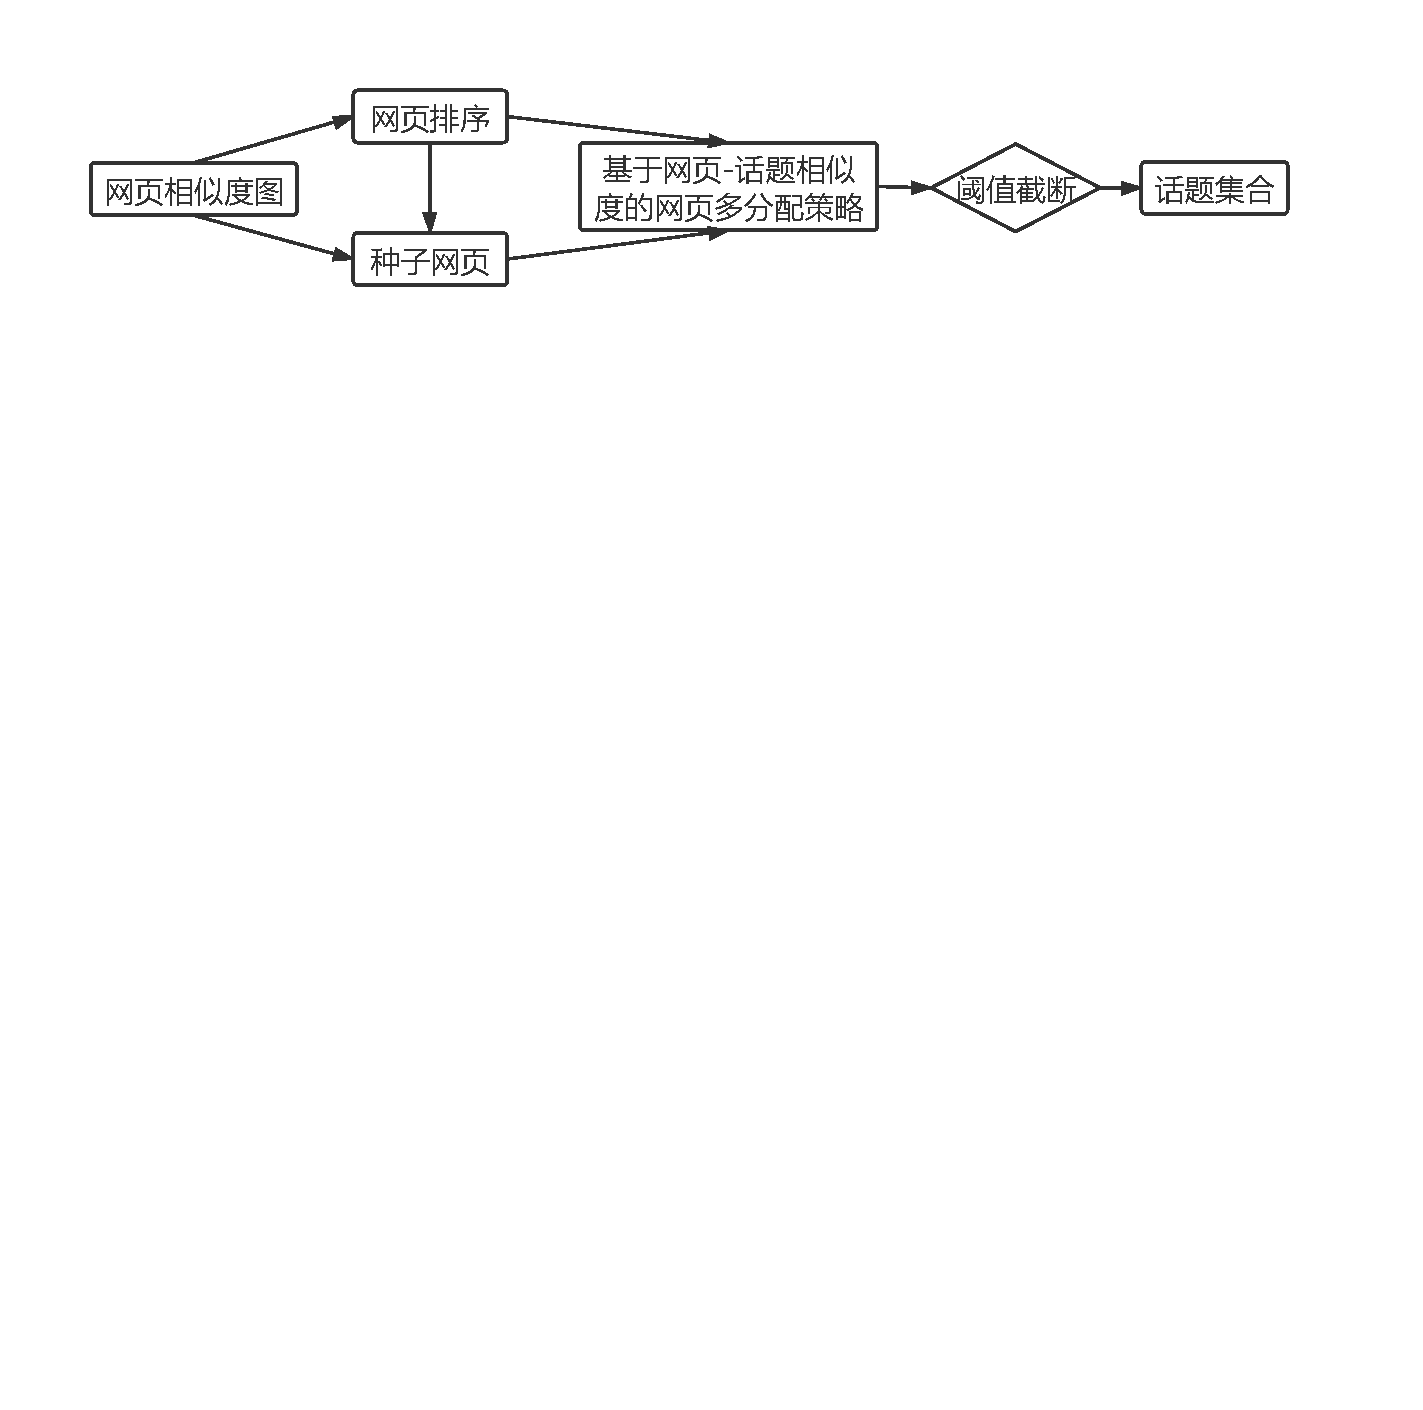
\includegraphics[width=1.0\textwidth]{LWTG.pdf}
    \caption{LWTG算法生成话题的框架图}
    \label{fig:LWTG}
\end{figure}

本论文中,我们提出两种度量网页和话题间相似度的方法,并将网页分配给相似度最高的$k$个话题来模拟网络话题在相似度空间中的L\'evy Walks特性:一些额外较低的相似度。

\subsection{寻找种子网页}
\begin{figure}[!htbp]
    \centering
    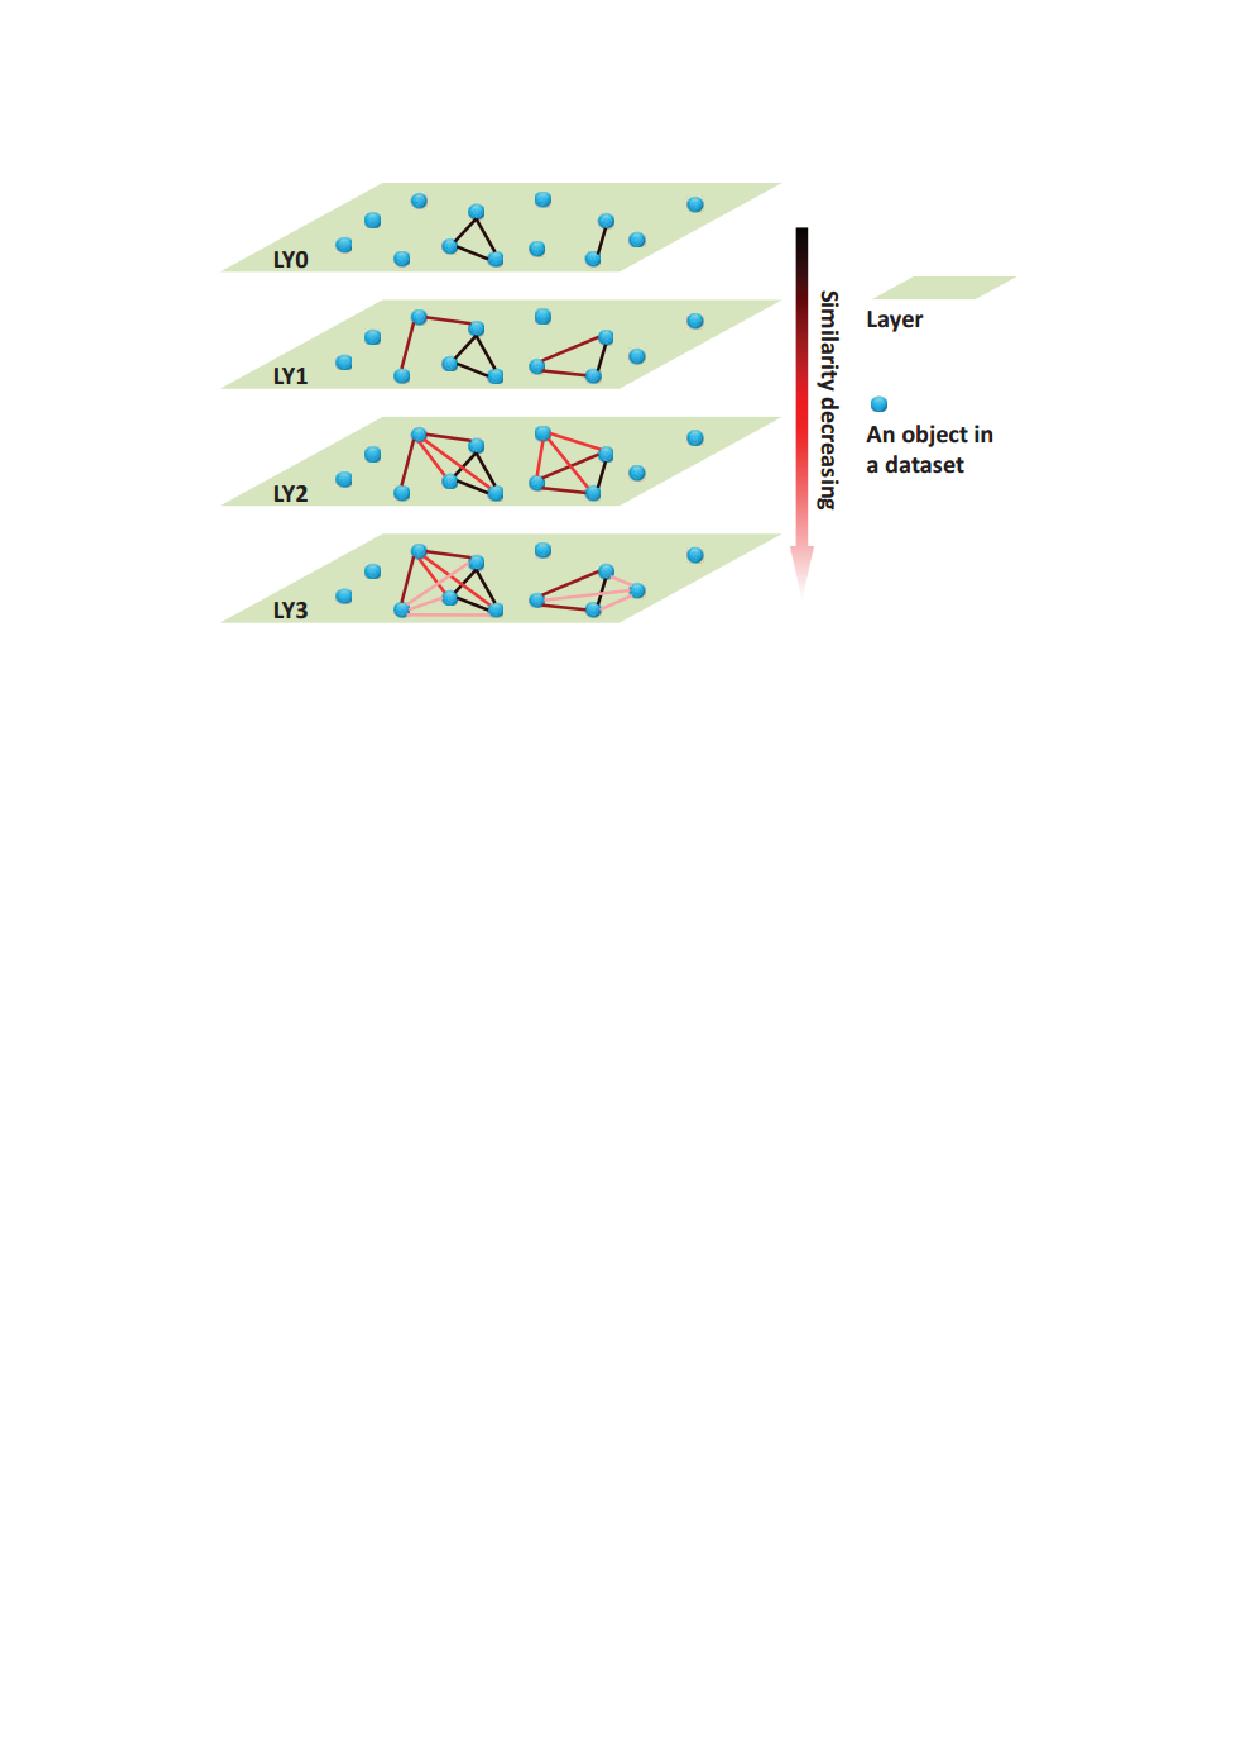
\includegraphics[width=1.0\textwidth]{similarity_cascade.pdf}
    \caption{基于相似度流的网络话题演化示意图}
    \label{fig:similarity_cascade}
\end{figure}
网络话题由初始核心事件不断在社交媒体上传播得以发展壮大。传播过程会逐渐吸收许多直接或者间接的外延信息。
网络话题的形成可以被看做是一种信息扩散的过程。而信息扩散的过程肯定会有一定的损失。我们使用相似度流来模拟这种信息扩散过程,扩散过程中信息的损失对应于相似度流中相似度值的较小。图\ref{fig:similarity_cascade}展示了网络话题基于相似度流的演化过程:话题初始时只有一两个网页,随后在较低的相似度上吸收更多的网页来形成更大的话题。随着演化的进行,吸收的网页的相似度越来越低。这种过程我们称之为相似度流扩散(Similarity Cascade, SC)。又因为不同用户之间的需求是不一样的,导致用户对话题的理解具有极大的差异。所以对同一个核心事件演化形成的话题,不同的用户所理解的话题的规模也是不一样的。

既然话题是由核心事件演化来的,那么我们希望能够通过代表该核心事件的种子网页,进而通过相似度流的扩散过程来模拟演化过程,最终生成话题。首要问题是如何判断一个网页能否作为种子网页?直观上理解,在一个由多个网页构成的话题中,其网页分布应该是尽可能均匀且紧凑的。均匀表示该话题内的网页之间的相似度较为接近,这是因为话题内的网页都是在为该话题服务的,所以它们应该是相似的,即相似度应该尽可能一致。紧凑表示该话题内的网页与话题应该是紧密相关,即相似度应该尽可能大。

受到论文[xxx]的启发,我们引进了站点熵率(Site Entropy Rate,SER)用来度量网页成为种子网页的概率。通过将相似度流从一个网页转移到另一个网页的过程模拟为全连接图中从一个站点转移到另一个站点的随机游走的过程,SER意味着从一个网页在一步内转移到其他网页的平均总信息转移量。而由种子网页吸收相似网页演化生成话题的过程中,越接近初始核心事件的网页,其通过相似度能够转移的平均总信息量也越大。SER的公式如下:
\begin{equation} \label{eq:SER}
SER_i = \pi_i\sum_{j\in<i>}-P_{ij}\log P_{ij}
\end{equation}
其中$P_{ij}=\frac{S_{ij}}{\sum_{j\in<i>}S_{ij}}$表示网页$w_i$转移到网页$w_j$的转移概率。$<i>\subset[1:N]$保存了s个与网页$w_i$最相似的网页索引。
公式\ref{eq:SER}表明SER可以被分为两个部分:稳态分布项和熵项。这两部分作用分别如下:
\begin{enumerate}
  \item[1)] 稳态分布项:$\pi_i = \frac{S_i}{S}$,其中$S_i=\sum_{j\in<i>}S_{ij}$是从网页$w_i$出发的所有相关相似度的和,$S = \sum_{i}\sum_{j\in<i>}S_{ij}$是相似度图中的所有网页及其最相似的s个网页的相似度的和。$\pi_i$被认为是网页$w_i$访问其他网页的频率;$\pi_i$越大,则表示由网页$w_i$经过一步演化的话题更加的紧凑;
  \item[2)] 熵项:$\sum_{j\in<i>}-P_{ij}\log P_{ij}$度量了网页$w_i$在一步内访问其他网页的不确定性。熵项越大,表明与网页$w_i$直接相连的其他网页的相似度分布更加均匀。
\end{enumerate}

\begin{figure}[!htbp]
    \centering
    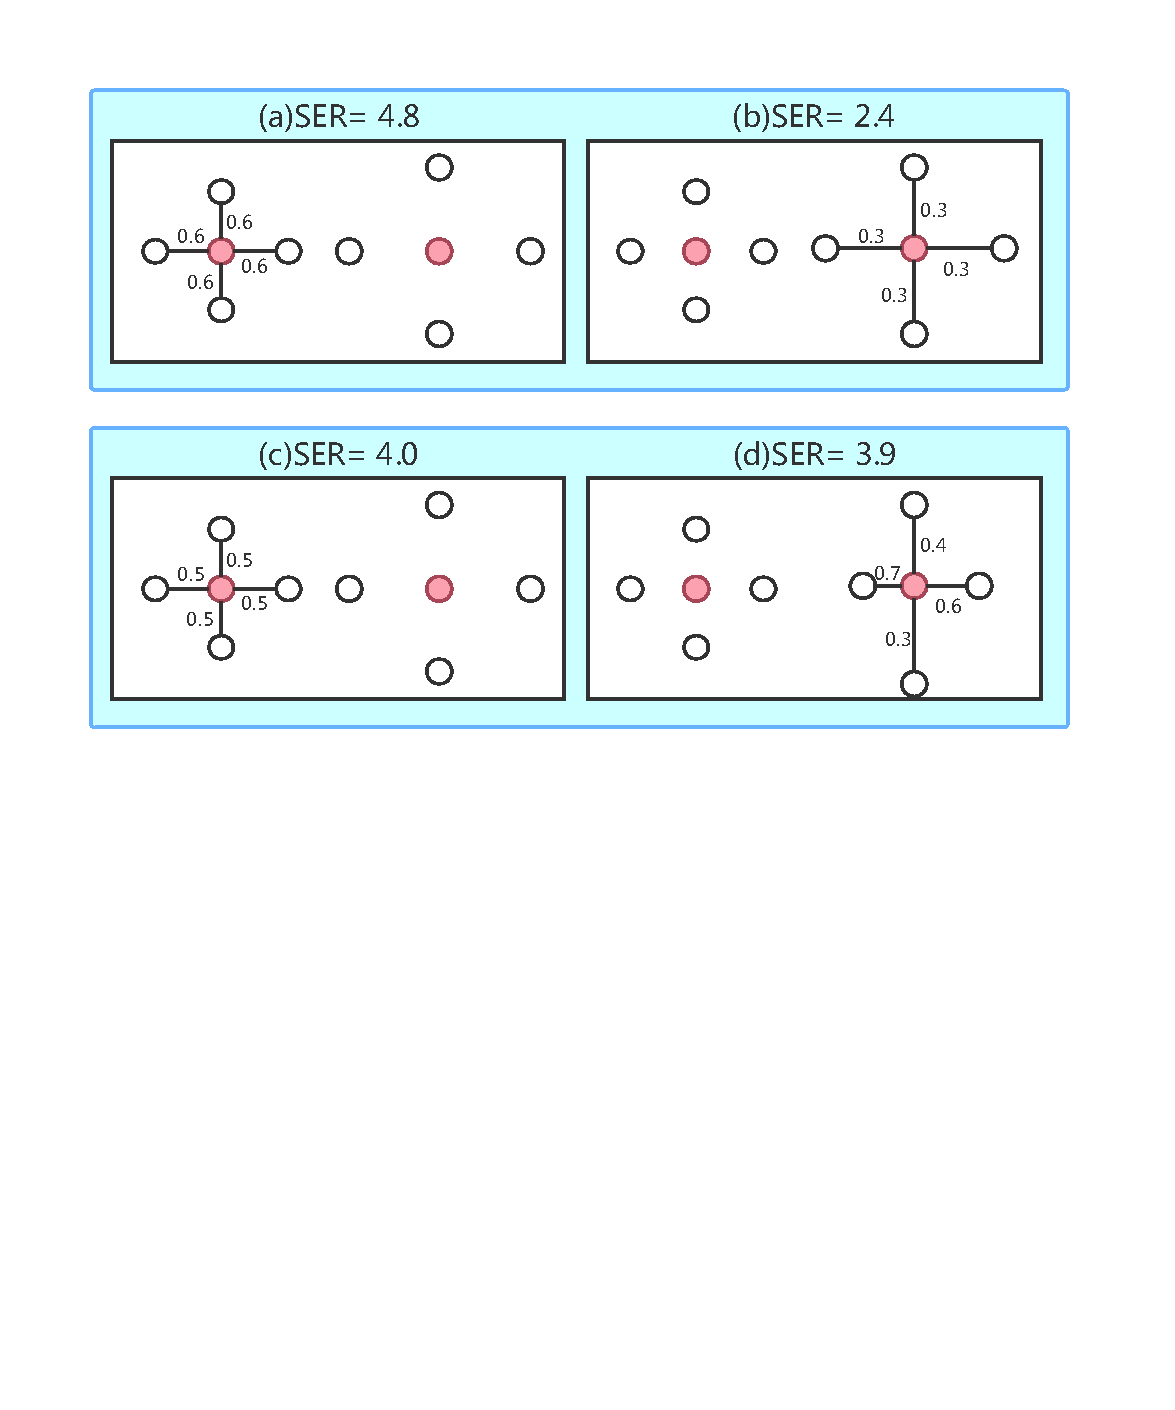
\includegraphics[width=1.0\textwidth]{seed_web_entropy.pdf}
    \caption{网页紧凑性和均匀性的SER评估}
    \label{fig:seed_web_entropy}
\end{figure}

SER由这两项的乘积构成。网页的SER越大,则表示其越有可能成为话题中的种子网页。如图\ref{fig:seed_web_entropy}所示,图中空心圈圈表示网页,红色实心圆圈表示要评估的网页,数字表示网页之间的相似度。从图(a)和图(b)可以看出在相同均匀分布的情况下(熵项一致),越紧凑的网页有更大的SER值。从图(c)和图(d)可以看出在相同紧凑性情况下(稳态分布项$\pi$一致),相似度分布越均匀的网页有更大的SER值。

在定义了SER作为网页成为种子网页的概率情况下,我们提出了一种基于关联度过滤的贪心算法来找到不同规模的种子网页。算法\ref{alg:greedysearchseedweb}展示整个搜索过程。算法的输入为相似度图,然后根据相似度图来计算每个网页的SER值。这里我们只需要选择与网页最相似的s个网页的相似度来计算SER值即可。因为SER仅用作一步内的相似度转移,而在一步内转移的网页应该是比较相似且数量比较少的,而不是全部的网页。所以这里我们只选择了s个最相似的网页来计算SER的值。另一个关联度参数d用来确定种子网页后,过滤与其最相似的d个网页。这么做是因为我们认为这d个最相似的网页可以在之后由该种子网页生长而得到。d值越大,产生的种子网页数量就越少。由于d值不好确定,同时为了更好地提高话题的召回率,我们使用多个不同的d值来产生多种规模的种子网页。算法输出为规模较小的种子网页集合。整个算法是基于SER值排序的贪心过滤算法:选择当前最优的种子网页,过滤与其最相似的d个网页,直到所有网页遍历结束。
\begin{algorithm}[!htbp]
    % \small
    \caption{基于关联度的种子网页贪心搜索算法}\label{alg:greedysearchseedweb}
    \hspace*{0.02in}{\bf Input:}
    相似度图 $G=(V,E,A)$,最相似网页个数$s$,关联度$d$\\
    \hspace*{0.02in}{\bf Output:}
    种子网页集合 $SW$,有序网页索引$SortedIndex$
    \begin{algorithmic}[1]
        % \State 初始化网页访问与否的的标记向量visit$\in \mathbb{R}^{N}$为False
        \State 初始化最终要生成的种子网页集合$SW$为空集
        \State 根据公式\ref{eq:SER}计算所有网页的SER
        \State 根据SER进行从大到小排序,得到有序且有连接的网页索引$SortedIndex$
        \State 找出与每个网页$w_i$最相似的$d$个网页索引,记为$\{i\}$
        \For{$i \in SortedIndex$}
        \If{网页$w_i$ 及其最相似的$d$个网页$w_{\{i\}}$ 未被访问} 
        \State $SW \leftarrow SW \bigcup w_i$
        \State 标记网页$w_i$及其最相似的$d$个网页$w_{\{i\}}$的状态为已访问
        \EndIf
        \EndFor
    \end{algorithmic}
\end{algorithm}


\subsection{网页多分配算法}

在产生种子网页后,我们提出了网页多分配算法来实现种子网页吸收相似网页,进而演化成话题。我们通过将网页分配给相似度最高的$k$个话题来模拟网络话题L\'evy Walks特性中额外较低的相似度。同时这个分配过程模拟了相似度流的扩散过程,所以我们采用了生成种子网页过程中产生的网页遍历顺序作为我们遍历网页的顺序。然后逐个进行网页分配。算法\ref{alg:multiallocateweb}展示了这个分配过程。其中对于每个待分配的网页,我们需要计算其与种子话题的相似度,希望这个相似度能够反映种子话题对网页的吸引程度。我们采用如下两种计算策略:
\begin{itemize}
  \item \textbf{Min}:我们定义网页$w_i$对种子话题$C_s$的相似度为该网页与话题内所有网页相似度的最小值,如公式\ref{eq:min}。我们认为在一个种子话题的所有网页中,存在的那个与网页$w_i$最不相似的网页$w_j$,如果连网页$w_j$与网页$w_i$的相似度都能取得较大值,那么整个种子话题$C_s$内的所有网页必然与网页$w_i$更加密切相关。即网页$w_i$就有更大的可能性归属于该种子话题$C_s$。
  \begin{equation}\label{eq:min}
    S_{is} = \min(S_{ij}),\ \ \ j \in C_s
  \end{equation}
  \item \textbf{AvgRate}:我们定义网页$w_i$对种子话题$C_s$的相似度为该网页所带来的平均相似度对比种子话题$C_s$当前平均相似度的比例。如公式\ref{eq:avgrate}。我们认为网页$w_i$如果能给种子话题$C_s$带来平均增加的相似度的比例越高,那么网页$w_i$与种子话题$C_s$必然更加密切相关。即网页$w_i$就有更大的可能性归属于该种子话题$C_s$。
  \begin{equation}\label{eq:avgrate}
    S_{is} = \frac{\text{Avg}(\sum_{j\in C_s}S_{ij})}{\text{Avg}(C_s)}
  \end{equation}
\end{itemize}

\begin{algorithm}[!htbp]
    % \small
    \caption{基于种子网页的网页多分配算法}\label{alg:multiallocateweb}
    \hspace*{0.02in}{\bf Input:}
    相似度图$G=(V,E,A)$,网页索引$SortedIndex$,种子网页集合$SW$,$k$\\
    \hspace*{0.02in}{\bf Output:}
    一系列话题集合$C$
    \begin{algorithmic}[1]
        \State 初始化空的话题集合C
        \State 初始化种子话题$C_s$($s\in SW$)及对应的阈值$th_s=1$
        \For{$i \in SortedIndex$}
        \State 计算网页$w_i$与每个种子话题$C_s$的相似度$S_{is}$
        \State $\{i\} \leftarrow \operatorname*{argmaxk}\limits_{s\in SW}(S_{is}, k)$\Comment{取与网页$w_i$最相似的$k$个种子话题的索引}
        \For{$s \in \{i\}$}
        \If{$IsCut(C_s, w_i, th_s)}$
        \State $C \leftarrow C \bigcup C_s$
        \State $C_s \leftarrow C_s \bigcup w_i$
        \State $th_s = \lfloor{\text{Avg}(C_s)\times10}\rfloor\div 10$
        \EndIf
        \EndFor
        \EndFor
    \end{algorithmic}
\end{algorithm}

得到网页与种子话题的相似度后,我们将网页分配给相似度最高的$k$个种子话题。公式\ref{eq:iscut}实现了函数$IsCut(\cdot)$,其中$th$使用了多层阈值来截断产生过完备的话题。阈值$th$在每一轮更新种子话题后重新赋值为当前种子平均相似度所处的层。比如说,之前种子话题的平均相似度$Avg(C_s)=0.76$,那么该种子话题所处的相似度层的阈值为$th=0.7$。如果新加的网页使得种子话题的平均相似度$Avg(C_s\cup w_i)=0.63$,那么由于更新后的种子话题不再属于原相似度层(即$0.63<0.7$),启动阈值截断,即将之前的种子话题作为生成的完整话题加入到话题集合中去。同时,更新当前相似度层阈值为$th=0.6$。
\begin{equation} \label{eq:iscut}
IsCut(\cdot) = 
\begin{cases}
1, & \text{Avg}(C_s\cup w_i) < th\\
0, & otherwise\\
\end{cases}
\end{equation}

基于上述两个算法,我们可以得到通过模拟L\'evy Walks来生成话题的算法\ref{alg:LWTG}。
\begin{algorithm}[!htbp]
    % \small
    \caption{基于L\'evy Walks的话题生成算法}\label{alg:LWTG}
    \hspace*{0.02in}{\bf Input:}
    相似度图$G=(V,E,A)$,最相似网页个数$s$,关联度集合D, 分配话题数$k$\\
    \hspace*{0.02in}{\bf Output:}
    过完备话题集合$C$ 
    \begin{algorithmic}
        \For{$d \in D$}
            \State 使用算法\ref{alg:greedysearchseedweb}\qquad \qquad \textbf{/* 寻找种子网页 */}
            \State 使用算法\ref{alg:multiallocateweb}\qquad \qquad \textbf{/* 通过网页多分配算法生成话题 */}
        \EndFor
    \end{algorithmic}
\end{algorithm}

\subsection{话题排序}

一旦相似度图$G(V,E,A)$构建完,我们通过算法\ref{alg:LWTG}生成候选话题集合。然后我们在泊松噪声的假设下,使用泊松去卷积算法(Poisson Deconvolution,PD)来评估每个话题的权重:
\begin{align} \label{eq:poisondeconvolution}
w_{ij} &\sim \textbf{Poisson}(a_{ij})\notag\\
s.t.: w_{ij} &= \sum_{k=1}^{K}\mu_kC_{k_{ij}}
\end{align}
其中$C_{k_{ij}}$表示第$k$个话题是否同时包含网页$w_i$和$w_j$。话题的兴趣度由$i_k=\mu_k\cdot|C_k|$计算得到,其中$C_k$是第$k$个话题包含的网页数量。具体细节参见章节\ref{chap:topicsSort}。




\subsection{时间复杂度分析}

我们提出的算法\ref{alg:LWTG}是基于L\'evy Walks的话题生成算法。主要包含寻找种子网页和网页多分配算法两部分。采用多粒度种子策略,其中$D$是种子网页的关联度集合,集合$D$的个数通常小于$10$。关联度越大,种子网页数量越少,通常从$1\sim10$中选取。

在寻找种子话题过程中,我们需要在只保留$knn$个近邻的相似度图中计算每个网页的SER值以及过滤相关网页,时间复杂度分别为:
\begin{itemize}
  \item 计算SER: $O(s\cdot knn\cdot N)$;
  \item 过滤网页: $O(d\cdot knn\cdot N)$;
\end{itemize}
其中$N$是网页总数。$knn$是每个网页要保留的近邻数,通常来说$knn$小于$100$。$s$是最相似的网页个数,通常小于$20$;d是要过滤的最相似网页个数(关联度),通常小于$10$。而对于大规模网络数据而言,网页数量通常是巨大的。所以综上可以得到寻找种子网页的时间复杂度为近似线性的$O(knn\cdot N)$。

在基于种子网页的网页多分算法中,我们需要针对每个网页计算两部分内容,分别是网页与种子话题的相似度以及网页分配给种子话题,时间复杂度分别是:
\begin{itemize}
  \item 计算网页和种子话题的相似度: $O(|topic|\cdot |SW|\cdot N)$;
  \item 将网页分配给k个话题: $O(k\cdot N)$;
\end{itemize}
其中$N$是网页总数。$|topic|$表示话题内包含的网页个数,通常小于$100$。$|SW|$是种子网页(种子话题)个数。
$k$是要分配的网页个数,通常小于$5$。所以综上可以得到网页多分配算法的时间复杂度为$O(|SW|\cdot N)$

从上面时间复杂度分析可以看出在算法\ref{alg:LWTG}中,基于种子网页的网页多分配算法占据主要的时间复杂度。因此我们提出的LWTG算法的时间复杂度为$O(|SW|\cdot N)$。种子网页的个数$SW$小于网页数$\frac{N}{2}$。这个时间复杂度对于大规模的网络数据来说是非常高效的。



\section{实验验证}
本节对我们提出LWTG算法在MCG-WEBV和YKS这两个数据集上展开实验。主要进行两方面的比较。第一个是跟两个最好的能够处理噪声数据的聚类算法进行对比;第二个是跟其他三个最好的网络话题检测算法进行对比。通过这两类对比来验证我们算法的性能。

\subsection{数据预处理}

对于MCG-WEBV数据集,我们使用其中的文本数据包括标题、标签和描述。首先过滤掉文本数据中的停用词,由于该数据集基本由英文构成,所以使用Python中的NLTK模块,对每个单词提取词干、统计tf-idf值作为单词权重,最后由tf-idf值生成每个网页的特征向量。

对于YKS数据集,基本由中文组成。所以需要采用NLPIR系统对文本数据进行预处理,包括分词、去停用词、处理同义词和扩展词等,然后统计每个词的tf-idf的值,再对每个网页生成特征向量。

\subsection{评测标准}
在评测标准上,我们使用以下两种评测指标:
\begin{itemize}
  \item 最高10个检测话题的$F_1$分数的均值-检测的话题数量(Top-10 $F_1$ v.s. Number of Detected Topics,NDT):对于每个检测得到的话题$D_t$,对应其最高匹配程度的真实标注的话题$G_t$,我们可以定义话题精确度$Precision$的公式\ref{eq:Precision}、话题召回率$Recall$的公式\ref{eq:Recall}和话题$F_1$的分数公式\ref{eq:F1}:
  \begin{align}
    \label{eq:Precision} Precision &= \frac{|D_t| \bigcap |G_t|}{|D_t|}\\
    \label{eq:Recall} Recall &= \frac{|D_t| \bigcap |G_t|}{|D_t| \bigcup |G_t|}\\
    \label{eq:F1} F_1 &= \frac{2\times Precision \times Recall}{Precision + Recall}
  \end{align}
  其中$|\cdot|$表示一个话题中的网页数目。

  \item 准确率-平均到每个话题上的误检率($Accuracy$ v.s. False Positives Per Topics,$FPPT$):准确率$Accuracy$的公式为\ref{eq:Accuracy},$FPPT$的公式为\ref{eq:FPPT}:
  \begin{align}
    \label{eq:Accuracy} Accuracy &= \frac{\#Successful}{\#Groundtruth} \\
    \label{eq:FPPT} FPPT &= \frac{\#Detected - \#Successful}{\#Successful}
  \end{align}
  其中话题被认为是正确检测到的标准由NIR(Normalized Intersected Ratio)指标衡量。NIR指标定义为公式\ref{eq:NIR}:
  \begin{equation}\label{eq:NIR}
    NIR = \frac{|D_t| \bigcap |G_t|}{|D_t| \bigcup |G_t|}
  \end{equation}
  当检测到的话题的$NIR$高于一定阈值(通常设为0.5)[xx]时,我们认为这是一个正确检测到的话题。对于$\# \triangle$表示对应集合$\triangle$的元素数量。
\end{itemize}

对于这两种评测指标,Top-10 $F_1$ v.s. NDT衡量算法检测到的最好的前10个话题的性能,但是并没有考虑到检测过程带来的误检率。而$Accuracy v.s. FPPT$综合衡量了所检测到的话题的准确率以及相应的平均每找到一个正确话题所带来的误检数。在这两种指标中,当具有相同Top-10 $F_1$分数或准确率时,更低NDT或FPPT的算法具有更优的话题检测性能。

\subsection{实验设置}

在实验中,我们选择了网页的文本数据进行词汇的tf-idf统计和编码,然后使用余弦距离构建相似度图。最后对每个网页只保留最相似的$knn$个网页的相似度值构建一个近邻
图。这里对MCG-WEBV数据集的$knn$设为100,最相似网页个数s设为10。对YKS数据集,由于噪声相比MCG-WEBV数据集更严重,所以近邻值$knn$设为15,最相似网页个数s设为15。在所有实验中,同时在相似度图上过滤噪声网页的阈值$\epsilon$设为0.1。跟种子粒度相关的关联度参数集合$D$设为${1,2,3,4}$。网页多分配的话题数$k$为2。

\subsection{与聚类算法的对比}

我们对比了LWTG算法与两个性能最好的能够处理噪声数据的聚类算法:
\begin{enumerate}
  \item[a)] Robust Spectral Clustering (RSC) for noisy data [xx]。这篇论文通过对相似度图的稀疏和隐式分解来处理噪声。然而,这种方法假设了噪声是稀疏的,但是在网络话题检测的场景下,大概$95\%$的数据都是噪声数据。
  \item[b)] Skinny-Dip (SD) [xx]。SD基于检验分布是否为单峰分布的Hartigan’s elegant dip test,从而得到一个有效的特征集来聚类。
\end{enumerate}

注意到RSC和SD算法不是为了检测网络话题而是为了从噪声数据中进行聚类。所以对于RSC,SD和LWTG的对比,主要是为了验证能处理噪声数据的聚类算法,能否有效地在海量噪声数据中检测到网络话题。在下面的实验中,对RSC,聚类个数设为真实话题个数。如MCG-WEBV数据集的$73$个真实话题和YKS数据集的$298$个真实话题。对于SD,聚类个数由算法自动确定。




\subsection{与网络话题检测算法的对比}

我们对比了LWTG算法与3个性能最好的网络话题检测算法:
\begin{enumerate}
  \item[a)] Multi-Modality Graph (MMG) [xx]。该算法属于多模态网络话题检测。Zhang等人首先利用视频的NDK信息和文本信息建立相似度图[xx],然后使用图转移算法[xx]进行话题检测。MMG假定了一个话题内的元素应该密切相关,所以,通常情况下MMG产生的话题规模较小。
  \item[b)] PD with Non-negative Matrix Factorization on Graph
(NMFG) [xx]。NMFG和LWTG最大的不同的是产生话题的方式。NMFG中使用基于图的非负矩阵分解(Non-negative Matrix factorization on Graph,NMG)[xx]在相似度级联上生成过完备话题。NMG在无噪声数据下的聚类非常耗时。
  \item[c)] Latent Poisson Deconvolution (LPD) [xx]。LPD算法在MCG-WEBV数据集和YKS数据集上均达到了当前最好的性能。相比单纯在PD上使用单一近邻图的方法,LPD利用多个近邻图来排序话题。这个证明了我们的方法可以在不利用多个近邻图的情况下达到可接受的结果。
\end{enumerate}

\section{小结}


\chapter{网络话题的快速排序} \label{chap:topicsSort}
\section{引言}
信息技术和移动网络的快速发展,使得社交媒体极大地促进了用户生成式数据(User-Generated Content ,UGC)\citep{pang-2013-unsupervised}的产生和传播。海量的UGC数据使得用户难以从中快速获取热点话题。

由这个实际问题出发,许多网络话题
检测算法\citep{pang-2013-unsupervised,zhang-2013-cross,pang-tao-2016-lpd}试图自动地将网页组织成有意义的话题。当前最好的网络话题检测算法是在相似度图上对话题的兴趣度进行排序\citep{pang-2013-unsupervised, pang-tao-2018-neurocomputing}。具体地说,泊松去卷积算法(Poisson Deconvolution,PD)通过扩散网页间的相似度来分配每个话题相应的权重\citep{pang-2013-unsupervised}。虽然相似度图可以不仅可以通过在线k近邻图($k$-Nearest Neighborhood Graph,$k$-N$^2$G)\citep{debatty-2016-fastonlineknn}构建,也能通过稀疏矩阵的方式存储。但是,一个严重的问题是PD算法在面对大规模网络数据时,无法进行高效地处理。这是因为PD算法迭代的每一轮必须使用所有的数据在内存中重构一个$N\times N$的浮点型矩阵,其中$N$是网页的数量。

那么,我们能否让PD算法在每次迭代的时候只使用一小部分样本呢?一个简单且有效的办法是随机优化\citep{hannah-2015-Stochastic}。这个办法能够带来至少两个好处:减少物理内存需求的同时,避免重构一个规模为$N\times N$的相似度图。然而,PD算法是通过期望最大化算法(Expectation-Maximization algorithm, EM)来优化的,它必须保持一个同相似度图一样规模的隐变量。

本章,我们提出了一个随机泊松去卷积算法(Stochastic Poisson Deconvolution,SPD)算法来处理大规模网络数据的话题检测问题。当每一轮迭代只能利用到一小部分样本时,SPD迭代地构建一个期望目标函数的代理函数。与此同时,只有一小部分随机采样的数据被用来更新代理函数。因此,通过避免把所有数据加载进内存,SPD算法显著地减少了运行时间。

据我们所知,这是第一个致力于解决网络话题检测中的泊松去卷积算法的可扩展性问题的算法。SPD算法不仅概念上简单而且实际上也非常有效。在一个大规模网络数据集中,SPD算法能够极大地缩短训练时间。比如在一个包含200,000个网页的数据集中,大概会有$12.6$倍的加速比。同时,在两个公开数据集上,SPD算法在话题检测效果上能够达到PD算法相同的水准。

\section{泊松去卷积算法(PD)}

先来回顾下泊松去卷积算法(Poisson Deconvolution,PD)\citep{pang-2013-unsupervised}。

给定一系列网页集合$\mathcal{X}=\{\mathbf{w}_1,\ldots,\mathbf{w}_N\}$,我们将这些网页转换成相似度图$G=(V,E,A)$,其中$V$表示网页集合$\mathcal{X}$,仿射矩阵$A(a_{ij}\in A)$表示将网页之间经过尺度化和截断后的相似度值,边集合$E(e_{ij}\in E$)表示网页间相似度值为非0的边。具体如何构建相似度图可以参考论文\citep{pang-tao-2016-lpd}。

通过相似度图$G$,可以生成一系列多粒度的话题集合$C_k(k=1,\ldots,K)$。一个话题$C_k$表示成:
\begin{equation}\label{eqt:ck}
C_{k} = c^{\top}_k{\circ} c_k
\end{equation}
其中指示向量$c_k\in\{0,1\}^{1\times N}$,$c_k$向量上第$i$位置上为$1$ 或者 $0$ 意味这话题$C_k$是否包含网页$w_i$。操作符$\circ$ 表示将矩阵$c^{\top}_k c_k$的对角元素设为0。

给定一系列话题集合$\{C_1,\ldots, C_K\}$和相似度图\mbox{$G=(V,E,A)$},话题$C_k$的权重$\mu_k$可以通过以下泊松噪声来学习:
\begin{equation} \label{eq:poissondeconvolution}
\begin{split}
r_{ij} & \sim \text{Poisson}(a_{ij})\\
where & \ \ r_{ij} = \sum_{k=1}^{K} \mu_k C_{k_{ij}}
\end{split}
\end{equation}
话题的兴趣度定义为$i_k=\mu_k\cdot |C_k|$,其中$|C_k|$表示话题$C_k$所包含的网页数量。

通过应用EM算法,PD算法可以通过如下迭代优化得到解:
\begin{equation} \label{eq:iterationofPD}
    \mu_k = \frac{\sum_{a_{ij}\in C_k} a_{ij} P_{k_{ij}}}{\sum_{a_{ij}\in C_k} C_{k_{ij}}}
\end{equation}
其中,$P_{k_{ij}}$($\sum_{k=1}^{K} P_{k_{ij}}=1$)是隐变量,并且,$P_{k_{ij}} = \frac{\mu_k C_{k_{ij}}}{\sum_{m=1}^{K}\mu_m C_{m_{ij}}}$\citep{pang-2013-unsupervised}。



\section{随机泊松去卷积算法(SPD)}

由于PD算法无法高效地处理大规模网络数据,我们提出了SPD算法以实现PD算法在大规模网络数据上的可扩展性。算法\ref{alg:SPD}展示了SPD算法的处理过程。通过假设相似度图中的边是独立同分布于一个未知的分布,我们在第$t$轮迭代时,从相似度图中随机采样一小批边集合$\bar{A}^t$作为该轮训练样本。然而,实际上,这一小批边是在随机排列训练集样本后,通过循环抽取得到的。这是因为我们很难获得真正独立同分布的样本。
\begin{algorithm}[!htbp]
    % \small
    \caption{随机泊松去卷积算法(SPD)}\label{alg:SPD}
    \hspace*{0.02in}{\bf Input:}
    相似度图 $G=(V,E,A)$,话题$C_k(k=1,...,K)$,批样本数$b$,迭代次数$T$\\
    \hspace*{0.02in}{\bf Output:}
    话题权重$\bm{\mu}$
    \begin{algorithmic}
        \State 初始化累积中间值$\bar{B}^0=\bar{D}^0=\bm{0}^{K\rm x 1}$
        \State 初始化参数$W=\bm{0}^{K\rm x 1}$, $\beta$,$\alpha$, $\bm{\mu}^0$
        \For{$t = 1,...,T$}
        \State 从相似度矩阵G中随机选择几行,构成每轮训练样本:$\bar{A}^t$
        \State 通过公式\eqref{eq:weightupdate}更新权重$w_k$
        \State 通过公式\eqref{eq:computebnkanddnk}计算临时变量$B^t_k$,$D^t_k$
        \State 更新累积中间值:
			\begin{center}$\bar{B}^t_k = (1-w^t_k)\bar{B}^{t-1}_k + w^t_kB^t_k$\end{center}
            \begin{center}$\bar{D}^t_k = (1-w^t_k)\bar{D}^{t-1}_k + w^t_kD^t_k$\end{center}
        \State 更新当前权重估计:$\mu^t_k = \frac{\bar{B}^t_k}{\bar{D}^t_k}$
        \EndFor
    \end{algorithmic}
\end{algorithm}

具体来说,PD算法公式\eqref{eq:poissondeconvolution}的目标函数等价于如下问题:
\begin{align} \label{eq:objectivefunction}
  &\quad\max{\ln \prod_{a_{ij} \in \bar{A}^t}\text{Poisson}(a_{ij})}  \notag\\
  &\Leftrightarrow\min \underbrace{\frac{1}{b}{\sum_{a_{ij} \in \bar{A}^t} \Big(\sum_{k=1}^{K}\mu_k C_{k_{ij}} - a_{ij}\ln \sum_{k=1}^{K}\mu_k C_{k_{ij}}\Big)}}_{f^t(\bar{A}^t,\bm{\mu})}
\end{align}
其中b是在相似度矩阵中这一小批样本$\bar{A}^t(\bar{A}^t\in \mathbb{R}^{b \rm x N})$的行数。

使用Jensen不等式,公式\eqref{eq:objectivefunction}中的似然函数的上界被用来作为代理函数:
\begin{align}
    f^t(\bar{A}^t,\bm{\mu}) &\leqslant{\underbrace{\frac{1}{b}\sum_{a_{ij} \in \bar{A}^t} \left(\sum_{k=1}^{K}\mu_k C^t_{k_{ij}} - a_{ij}\sum_{k=1}^{K} P^t_{k_{ij}} \ln \frac{\mu_k C^t_{k_{ij}}}{P^t_{k_{ij}}}\right)}_{J^t(f^t,\bm{\mu}^{t-1})}}
\end{align}
其中$C^t_{k_{ij}}$意味着与采样边相关的第k个话题,$P^t_{k_{ij}}$($\sum_{k=1}^{K}P^t_{k_{ij}}=1)$是第$t$轮迭代时的隐变量,并且$P^t_{k_{ij}} = \frac{\mu^{t-1}_k C^t_{k_{ij}}}{\sum_{k=1}^{K}\mu^{t-1}_k C^t_{k_{ij}}}$。这里,我们要注意到,并非每条边均能对所有话题产生影响。一般情况下,每条边只能影响到包含该边的少数几个话题。也就是说,每一小批边样本只能影响一小部分话题,即只需更新该部分被影响的话题权重。

代理函数$J^t(f^t,\mu^{t-1})$ 关于$\mu_k$的梯度为:
\begin{equation} \label{eq:computebnkanddnk}
    \frac{d}{d\mu_k}J^t(f^t,\bm{\mu}^{t-1})=\underbrace{\frac{1}{b}\sum_{a_{ij}\in \bar{A}^t}C^t_{k_{ij}}}_{D^t_k} - \underbrace{\frac{\frac{1}{b}\sum_{a_{ij}\in \bar{A}^t} a_{ij}P^t_{k_{ij}}}{\mu_k}}_{B^t_k}
\end{equation}
其中$D^t_k\in \mathbb{R}^{1 \rm x 1}$和$B^t_k\in \mathbb{R}^{1 \rm x 1}$是临时变量。

\begin{proposition}
   (迭代更新过程)给定临时变量$B^t_k$和$D^t_k$,按如下方式迭代更新$\mu_k$:
	\begin{equation} \label{eq:updatemu}
	    \mu^t_k = \frac{\bar{B}^t_k}{\bar{D}^t_k} \quad s.t.:\quad k \in \{k|\exists C^t_{k_{ij}} \neq 0\}
	\end{equation}
	其中
	\begin{equation} \label{eq:iterativeupdating}
	\begin{split}
	    \bar{B}^t_k \leftarrow (1-w^t_k)\bar{B}^{t-1}_k + w^t_kB^t_k\\
	    \bar{D}^t_k \leftarrow (1-w^t_k)\bar{D}^{t-1}_k + w^t_kD^t_k
	\end{split}
	\end{equation}
	其中,第$t$轮迭代的权重$w^t_k$为:
	\begin{equation} \label{eq:weightupdate}
	    w^t_k = \beta\sqrt{\frac{1+\alpha}{W_k+\alpha}}
	\end{equation}
	其中
	$\beta \in (0,1]$,$\alpha \geq 0$,$W_k = W_k + 1$,$k$为那些受到影响的话题索引。
\end{proposition}

\begin{proof}
    遵循论文SMM\citep{mairal-2013-SMM}的建议,近似代理函数和当前估计的结合得到如下公式:
    \begin{equation} \label{eq:exponentiallyweightedmovingaverage}
    \bar{J}^t_k \leftarrow (1-w^t_k)\bar{J}^{t-1}_k + w^t_k J^t_k
	\end{equation}
	通过最小化公式\eqref{eq:exponentiallyweightedmovingaverage},可以得到$\mu^t_k = \arg \min \bar{J}^t_k(\mu)$。这个过程可以根据如下推导得到:

	当$t=m$, 通过最小化公式\eqref{eq:exponentiallyweightedmovingaverage},同时利用公式\eqref{eq:computebnkanddnk},\eqref{eq:updatemu},\eqref{eq:iterativeupdating},我们可以得到:
	\begin{equation}
	\mu^m_k = \frac{(1-w^m_k)\bar{B}^{m-1}_k+w^m_kB^m_k}{(1-w^m_k)\bar{D}^{m-1}_k+w^m_kD^m_k} = \frac{\bar{B}^m_k}{\bar{D}^m_k}
	\end{equation}
	最终,不失一般性,我们可以得到$\mu^t_k$在第$t$轮的更新过程\eqref{eq:updatemu},\eqref{eq:iterativeupdating},\eqref{eq:weightupdate}。
\end{proof}

权重参数$w$在近似代理函数公式\eqref{eq:exponentiallyweightedmovingaverage}中扮演了指数加权移动平均的作用(Exponentially Weighted Moving Average,EWMA)。EWMA是一无限脉冲响应过滤器,代表了指数衰减的权重。注意到旧代理函数的权重呈现指数衰减但不会减少到0。权重$w$反映了当前代理函数的重要性,权重$1-w$反映了旧代理函数的重要性。因此,代理函数越旧,其对应的权重值$w$越小。

\section{异步并行的随机泊松去卷积算法}

由于网络数据规模庞大,导致SPD算法可能还是不够高效。同时,多核系统已经普遍存在。所以,通过设计一个异步策略来并行化SPD算法,我们提出了一种基于多核系统的异步并行的SPD算法(AsySPD)。

假设我们有$p$个可以访问一个共享内存的线程(进程),待求解的话题权重$\mu$、话题更新次数$W$以及累积中间值$\bar{B}$和$\bar{D}$位于共享内存中。同时对于每个线程,都可以访问共享内存中的变量,并且可以随机选择训练集中的样本。我们还进一步假设对共享内存中的向量型变量进行一致性读操作。

算法\ref{alg:AsySPD}展示了我们的AsySPD算法。在$t$-th轮更新时,对于每个线程,均随机采样一批样本,并且进行独立计算和更新共享内存中的变量。$M$是所有线程在一轮数据集内更新的总次数。对于每个线程的每次独立更新,与算法\ref{alg:SPD}几乎一致,只是有些全局性变量(如话题更新次数$W$和累积中间值$\bar{B}$、$\bar{D}$)位于共享内存中,所有线程均可以对其进行更新。最后在更新共享内存中的$\bm{\mu}$时,使用$\bm{\mu_k} = \frac{\bm{\mu_k}+\bm{\mu}^m_k}{2}$公式来融合当前线程带来的更新。
\begin{algorithm}[!htbp]
    % \small
    \caption{异步并行随机泊松去卷积算法(AsySPD)}\label{alg:AsySPD}
    \hspace*{0.02in}{\bf 初始化:}
    $p$个线程,共享内存中的$\bm{\mu}$、$W$、$\bar{B}$、$\bar{D}$\\
    \hspace*{0.02in}{\bf Output:}
    共享内存中的$\bm{\mu}$
    \begin{algorithmic}
        \For{$t = 1,...,T$}
          \State 对于每个线程,执行
          \For{$m = 1,...,M$}
            \State 从相似度矩阵G中随机选择$b$行,构成每轮训练样本:$\bar{A}^m$
            \State 更新$W_k = W_k + 1$,其中$k$为受到样本$\bar{A}^m$影响的话题索引
            \State 通过公式\eqref{eq:weightupdate}计算临时权重$w^m_k$
            \State 通过公式\eqref{eq:computebnkanddnk}计算临时变量$B^m_k$,$D^m_k$
            \State 通过公式\eqref{eq:iterativeupdating}更新$\bar{B}_k$和$\bar{D}_k$
            \State 计算临时$\bm{\mu}^m_k = \frac{\bar{B}_k}{\bar{D}_k}$
            \State 更新$\bm{\mu_k} = \frac{\bm{\mu_k}+\bm{\mu}^m_k}{2}$
          \EndFor
        \EndFor
    \end{algorithmic}
\end{algorithm}



\section{实验验证}

\subsection{数据集、特征、评估标准、实验设置}

\begin{table}[t!]
\begin{center}
\caption{数据集的统计信息汇总} \label{tab:dataset}
\begin{tabular}{|c|c|c|c|c|}
  \hline
  Data sets & \#Webpage & \#Topics & $knn$ & Sparsity(\%)\\
  \hline\hline
  MCG-WEBV & 3660 & 4240 & 100 & 2.73\\
  \hline
  YKS & 8660 & 5252 & 20 & 0.273\\
  \hline
\end{tabular}
\end{center}
\end{table}
\textbf{数据集:} 在本章实验中,我们仍然使用MCG和YKS两个数据集来评估我们提出的SPD算法。同时为了验证SPD算法在大规模网络数据上的效率,我们通过在对角位置叠加50个MCG-WEBV数据集的相似度矩阵,最终得到一个大约包含200,000个网页的人工数据集的相似度矩阵。两个真实数据集的统计信息如表\ref{tab:dataset}所示。

\textbf{特征:} 在数据预处理阶段,仍然对MCG和YKS数据集提取文本数据的TF-IDF特征。然后使用余弦距离计算网夜间的相似度。接着保留与每个网页最相似的$k$个网页的相似度值,其余置为0,最终生成一个$k$近邻的相似度图。

\textbf{评估标准:} 仍然使用Top10-$F_1$ v.s. Number of Detected Topics ($NDT$)\citep{cao-2011-tracking} 和 $Accuracy$ v.s. False Positive Per Topic ($FPPT$)\citep{pang-2013-unsupervised}。当两个方法有相同的Top10-$F_1$或$Accuracy$分数后,拥有更小$NDT$或者$FPPT$的算法有更好的性能。同时,对于算法运行时间效率方面的评估,我们采用了目标函数的收敛曲线。

\textbf{实验设置:} 所有实验使用了相同的实验设置,比如相似度图和待排序话题集合。所有实验代码使用python语言在3.6G Hz CPU和32G内存的电脑上运行。


\subsection{复杂度分析}

对PD算法,需要在内存中分配一个$N\times N$的浮点型矩阵来存储重构的相似度图。因此,PD算法的空间复杂度和时间复杂度分别为$O(N^2)$ and $O(TN^2)$。作为对比,SPD算法只需要在内存中保存一个规模为$b\times N$的浮点型矩阵,其中$b\times N$表示每次采样的一小批边样本规模(比如,$\bar{A}^t\in \mathbb{R}^{b \rm x N}$)。所以SPD算法的空间复杂度为$O(bN)$ $(b\ll N)$。


\subsection{在人工数据集上对比PD和SPD}

为了评估SPD算法的运行效率,我们构造了一个较大规模的人工数据集。本章中,如果一个算法前后两轮迭代的目标似然函数的对数值的变化小于$10^{-5}$,那么我们认为该算法收敛到了一个局部极小值。同时定义算法A对算法B的加速比是算法收敛到局部极小值时的CPU运行时间之间的比值,如公式\eqref{eq:speedup}:
\begin{equation}\label{eq:speedup}
speedup = \frac{\text{算法A收敛到局部极小值时的CPU运行时间}}{\text{算法B收敛到局部极小值时的CPU运行时间}}
\end{equation}

\begin{figure}[!htbp]
    \centering
    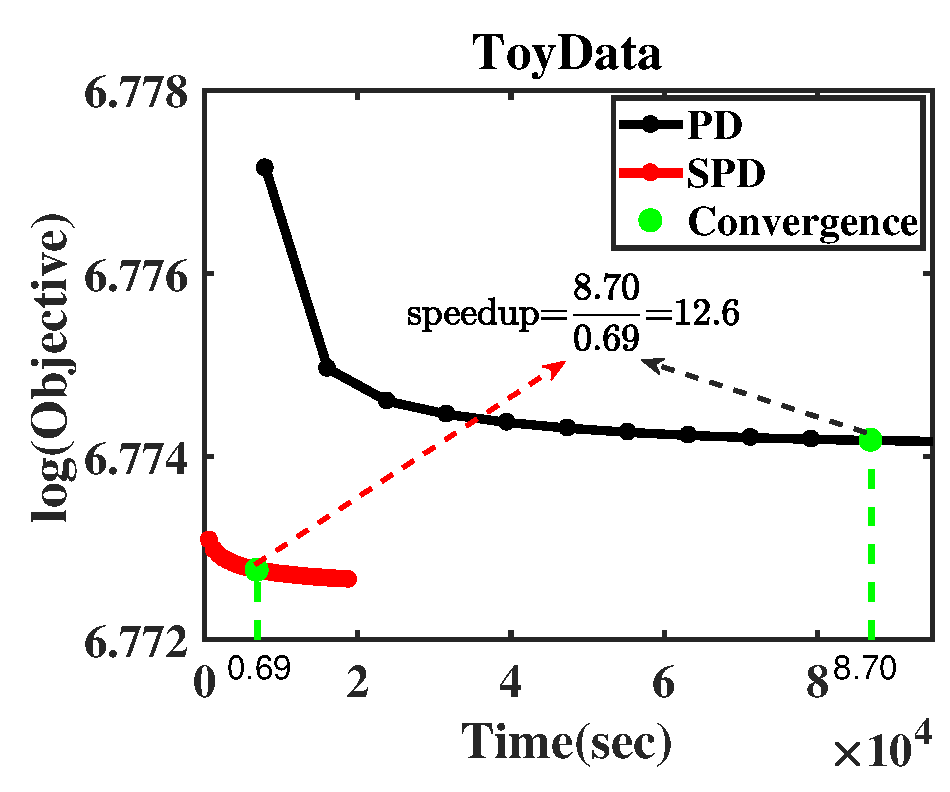
\includegraphics[width=0.7\textwidth]{ToyDataset_Objective}
    \caption{PD和SPD算法在ToyData上的收敛对比}
    \label{fig:ToyDataset_Objective}
\end{figure}
图\ref{fig:ToyDataset_Objective}表明,就收敛速度而言,SPD算法显著由于PD算法。在我们的评估中,SPD算法相比PD算法会有大概12.6倍的加速比。而且,在每一轮迭代,虽然PD算法的目标函数下降得更多,但是我们的随机方法相比批处理方法使用更少的训练时间。这是因为在每一轮迭代更新的时候,PD算法使用所有的数据去进行一个精确的更新,而SPD算法只使用一小部分样本去进行一个近似的更新。当训练一个大规模的网络数据时,由于计算效率和内存限制的原因,PD算法将会比SPD算法花费更多的时间来使用一轮数据集进行更新。因此,在处理大规模网络数据时,SPD算法的收敛速度会比PD算法快很多。这同时也验证了公式\eqref{eq:exponentiallyweightedmovingaverage}作为损失函数的优点:一个算法无需花费太多的时间去精确地最小化经验损失。另外,就像梯度下降一样,PD算法同样遭遇局部极小值问题,而SPD算法可以更好地避免该问题,从而能够收敛到一个更小的局部极小值。


\subsection{在MCG-WEBV和YKS上对比PD和SPD}

对于话题排序效果,图\ref{fig:cmp-accuracy}使用$Accuracy$ v.s. $FPPT$在MCG-WEBV和YKS数据集上对比了PD算法和SPD算法的结果。从图\ref{fig:cmp-accuracy}可以看出SPD算法的话题排序效果与PD算法相似。同时图\ref{fig:cmp-top10}进一步使用Top10-$F_1$ v.s. $NDT$证明了SPD算法的排序效果不比PD算法差。综上,说明我们的SPD算法可以达到和PD算法相似的话题排序效果。
\begin{figure}[!htbp]
    \centering
    \begin{subfigure}[b]{0.5\textwidth}
      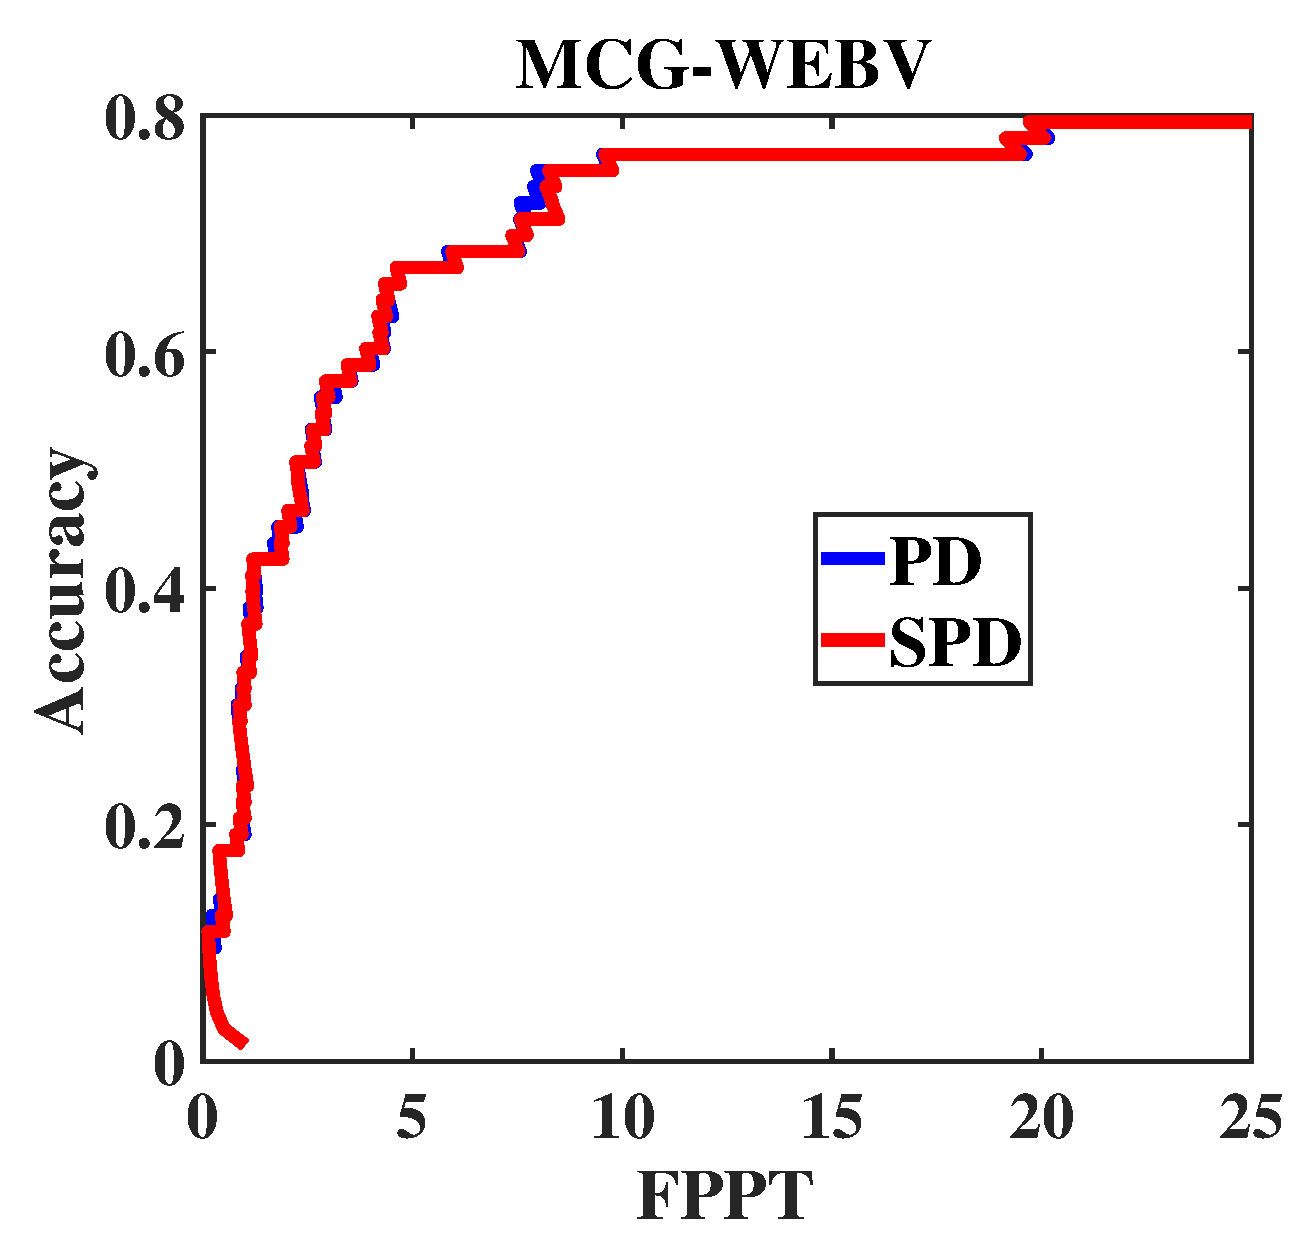
\includegraphics[width=\textwidth,height=0.95\textwidth]{MCG_Accuracy}
      \caption{}
      \label{fig:accuracycmponmcg}
    \end{subfigure}%
    \begin{subfigure}[b]{0.5\textwidth}
      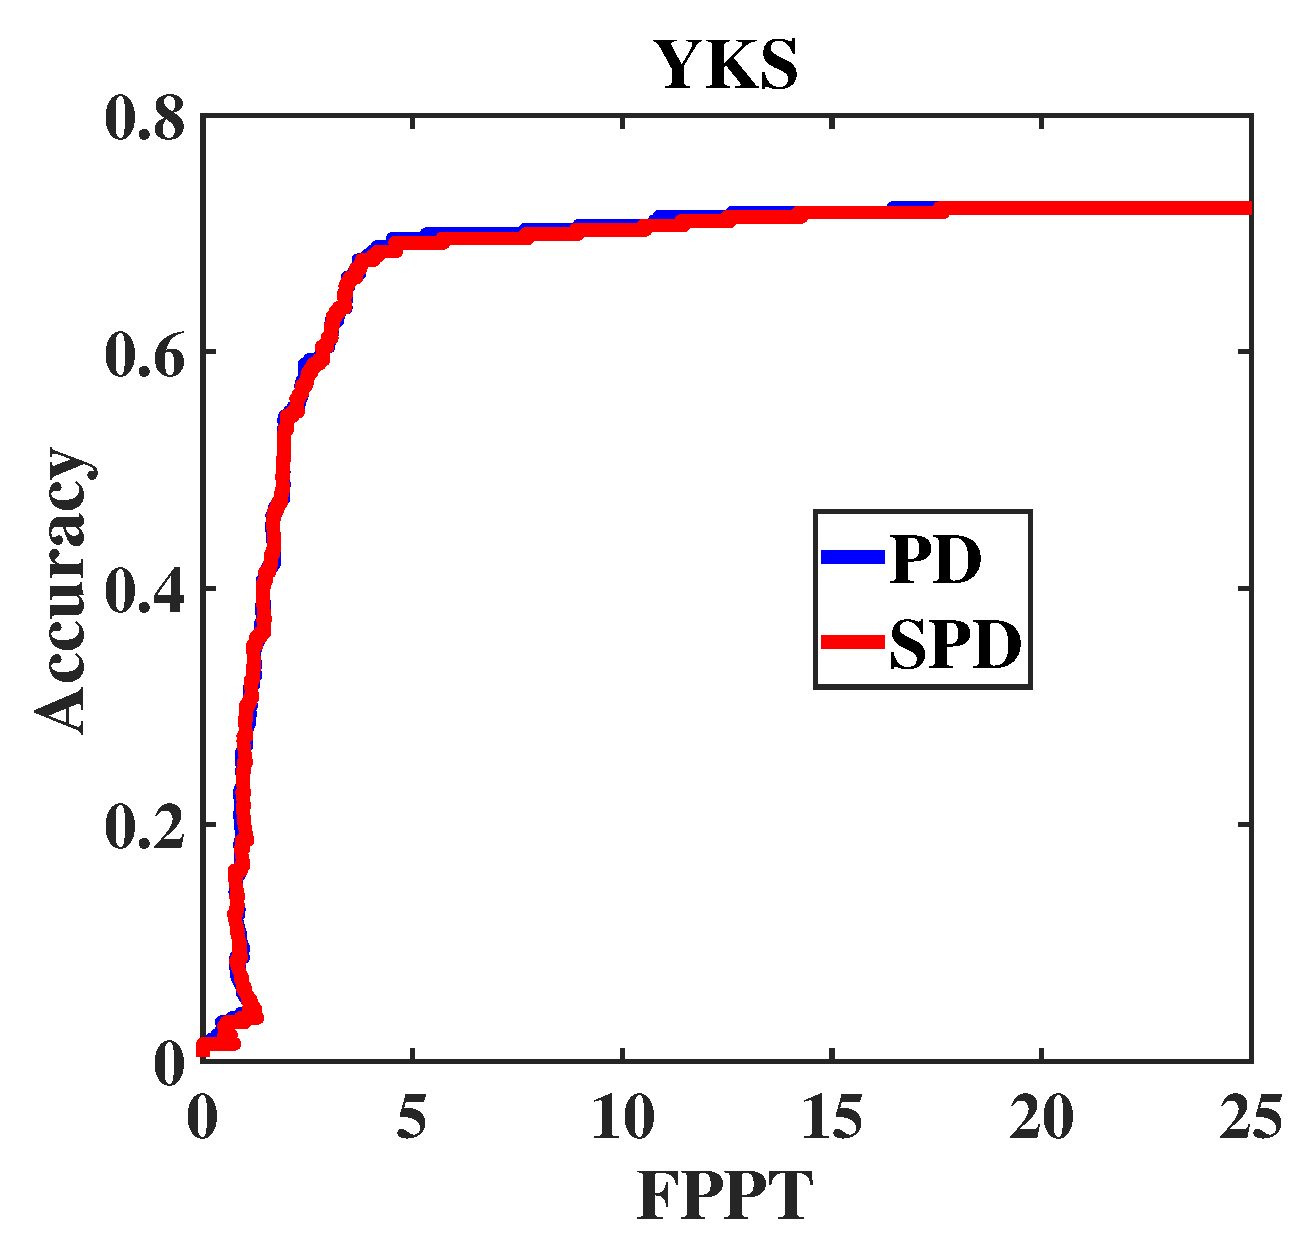
\includegraphics[width=\textwidth,height=0.95\textwidth]{YKS_Accuracy}
      \caption{}
      \label{fig:accuracycmponyks}
    \end{subfigure}%
    % ~% add desired spacing
    \caption{使用$Accuracy$ v.s. $FPPT$对比PD和SPD算法}
    \label{fig:cmp-accuracy}
\end{figure}
\begin{figure}[!htbp]
    \centering
    \begin{subfigure}[b]{0.49\textwidth}
      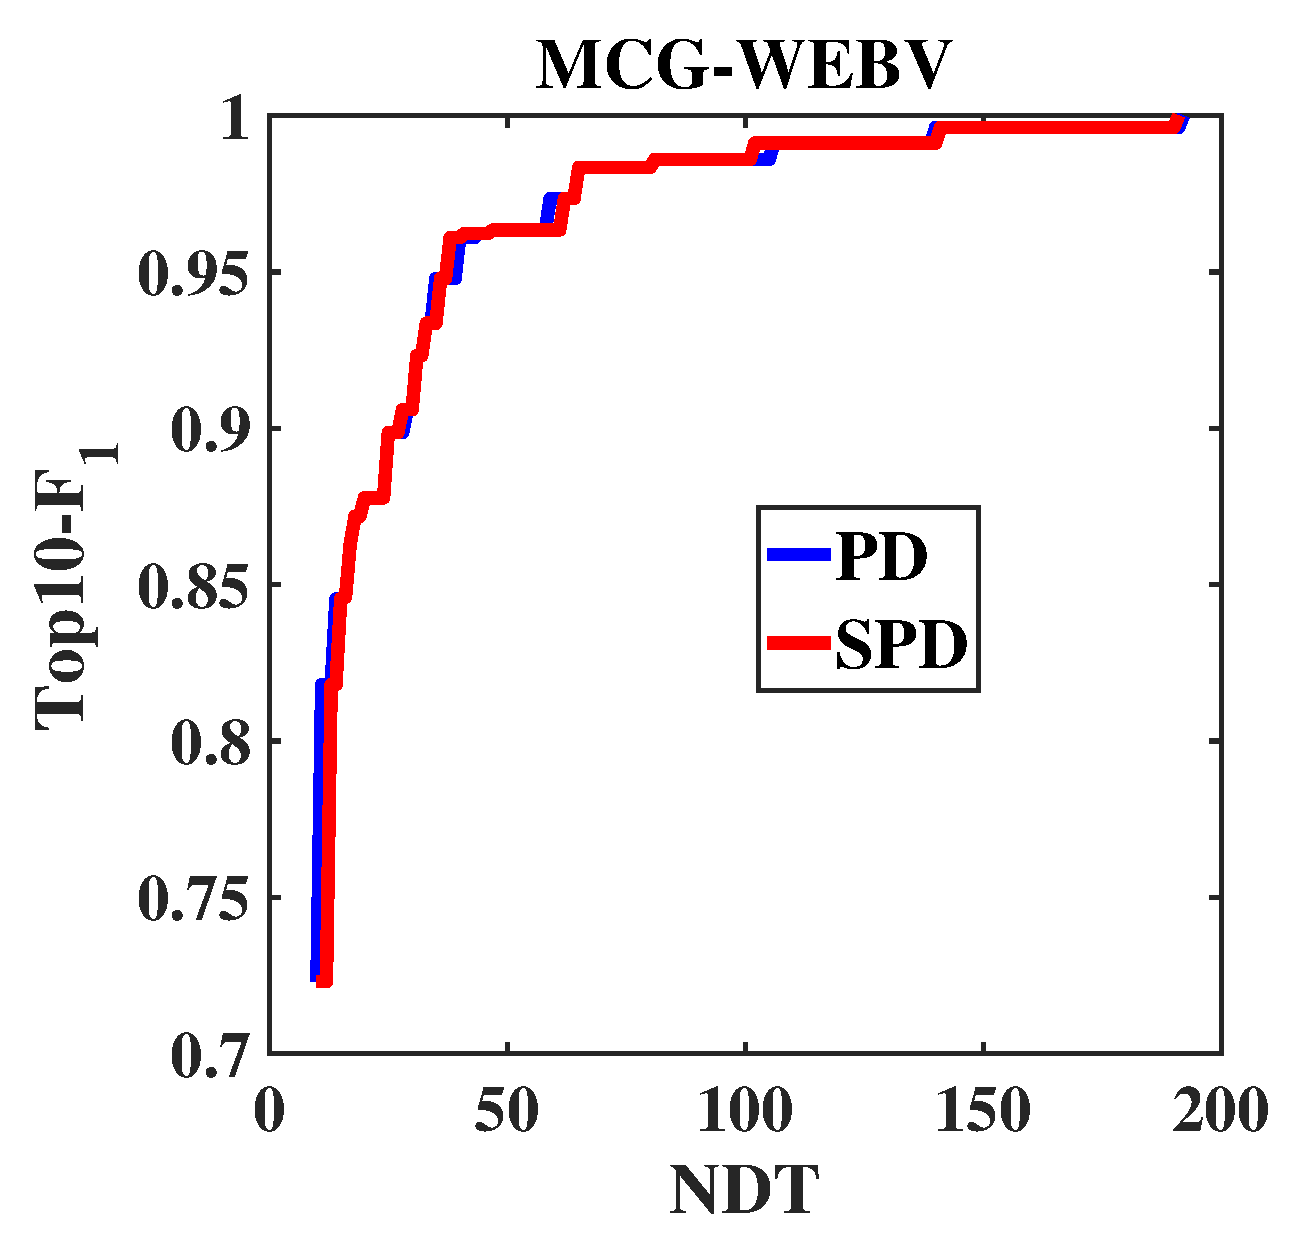
\includegraphics[width=\textwidth,height=0.95\textwidth]{MCG_Top10}
      \caption{}
      \label{fig:top10cmponmcg}
    \end{subfigure}
    % ~% add desired spacing
    \begin{subfigure}[b]{0.49\textwidth}
      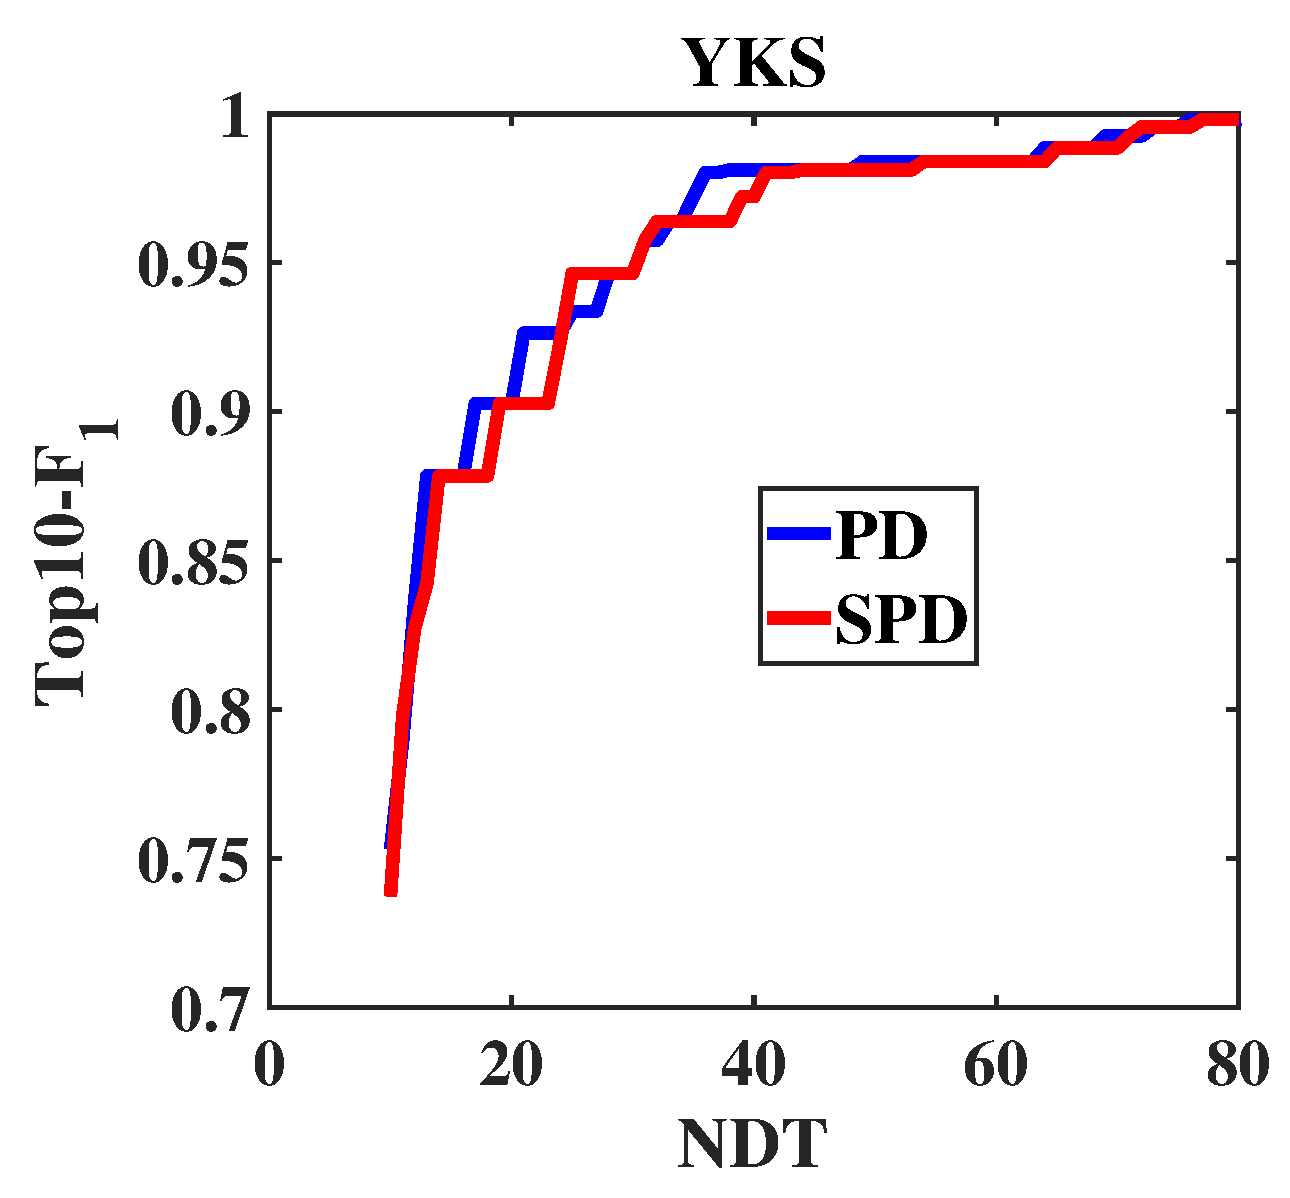
\includegraphics[width=\textwidth,height=0.95\textwidth]{YKS_Top10}
      \caption{}
      \label{fig:top10cmponyks}
    \end{subfigure}
    \caption{使用Top10-$F_1$ v.s. $NDT$对比PD和SPD算法}
    \label{fig:cmp-top10}
\end{figure}

对于话题排序效率,图\ref{fig:cmp-objective}对比PD算法和SPD算法在MCG-WEBV和YKS数据集上的收敛情况。从这两幅图中可以看出SPD算法可以收敛到一个更低的对数似然函数值。这意味这SPD算法可以在保证算法排序效果的同时使目标函数收敛到更低的值。但是由于这两个数据集都很小,SPD算法的随机采样优势没能发挥出来,所以导致SPD算法训练一遍数据集花费的时间比PD算法多。所以在处理小规模网络数据时,SPD算法收敛会比PD算法慢。但是,在处理大规模网络数据时,SPD算法的随机优势就能得以发挥使其收敛速度比PD算法快。
\begin{figure}[!htbp]
    \centering
    \begin{subfigure}[b]{0.5\textwidth}
      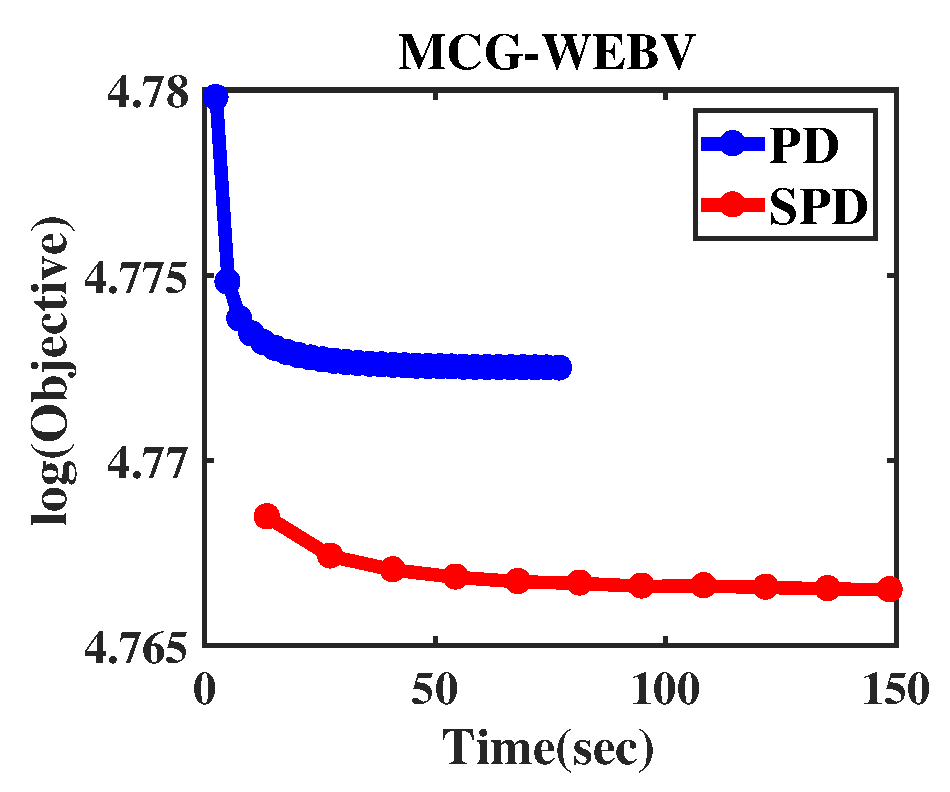
\includegraphics[width=\textwidth,height=0.95\textwidth]{MCG_Objective}
      \caption{}
      \label{fig:objectivecmponmcg}
    \end{subfigure}%
    \begin{subfigure}[b]{0.5\textwidth}
      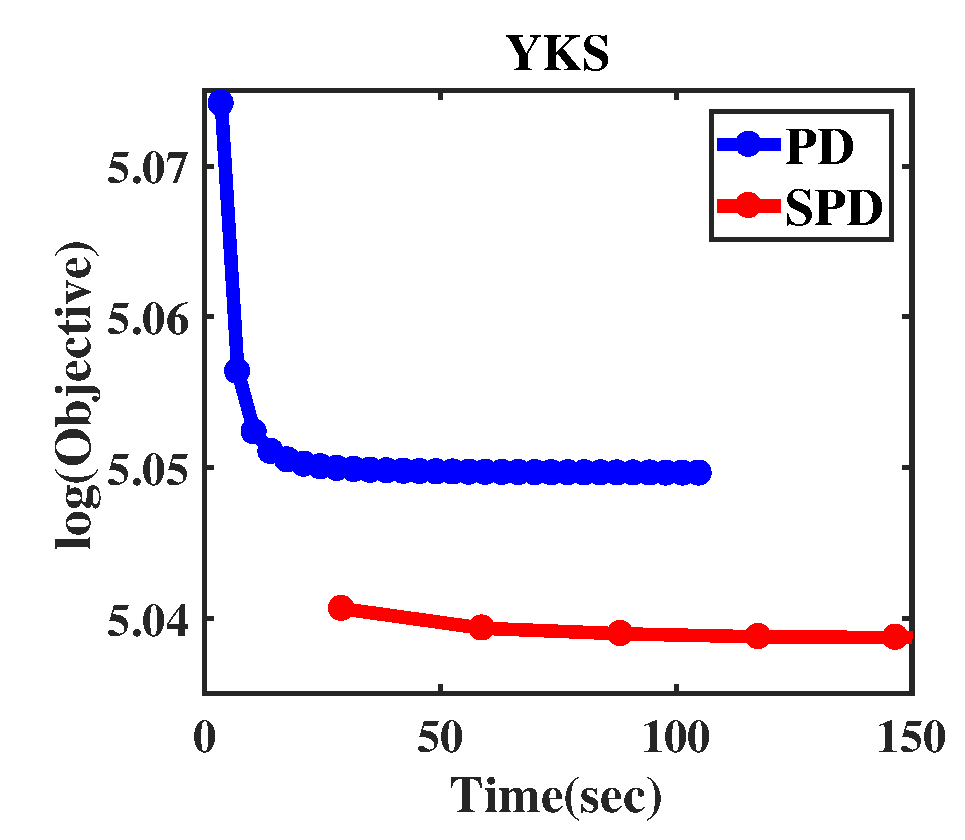
\includegraphics[width=\textwidth,height=0.95\textwidth]{YKS_Objective}
      \caption{}
      \label{fig:objectivecmponyks}
    \end{subfigure}%
    \caption{使用目标函数收敛曲线对比PD和SPD算法}
    \label{fig:cmp-objective}
\end{figure}


\subsection{参数分析}

\subsubsection{批样本数量$b$:}

图\ref{fig:minibatch-Objective}展示了在MCG-WEBV数据集上,不同的批样本数量$b$的大小对SPD算法目标函数收敛曲线的影响。从中可以看出不同的批样本数量$b$均收敛到一个局部极小值。此外,$b$值越小,对数目标函数值也会收敛到更低的程度。一个可能的解释是更小的批样本数量会带来更大的随机性,使得SPD算法更有可能逃离较差的局部极小值,到达一个相对较好的局部极小值。
\begin{figure}[!htbp]
    \centering
    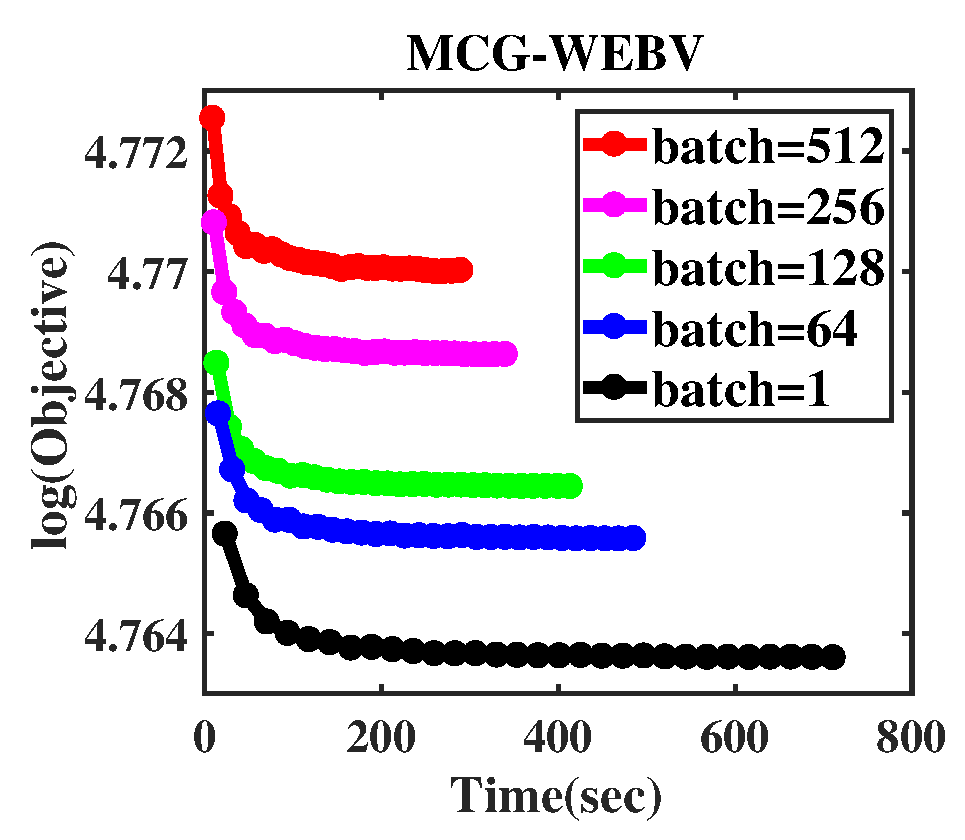
\includegraphics[width=0.7\textwidth]{minibatch_Objective}
    \caption{不同批样本数量$b$对目标函数收敛曲线的影响}
    \label{fig:minibatch-Objective}
\end{figure}

有趣的是,图\ref{fig:minibatch-two-metric}显示不同大小的批样本数量均能获得相似的$Accuracy$和Top10-$F_1$值。可能的原因是即使不同的$b$值导致最终的话题权重$\mu$值的分布不同,对数目标函数值不同。但是,只要这些话题权重$mu$值的相对大小分布几乎不变,即对$\mu$值排序后的所处位置在不同批样本数量时几乎不变,那么就有可能达到相似的$Accuracy$和Top10-$F_1$。因此,批样本数量$b$的大小不会影响SPD算法的话题排序性能。
\begin{figure}[!htbp]
    \centering
    \begin{subfigure}[b]{0.5\textwidth}
      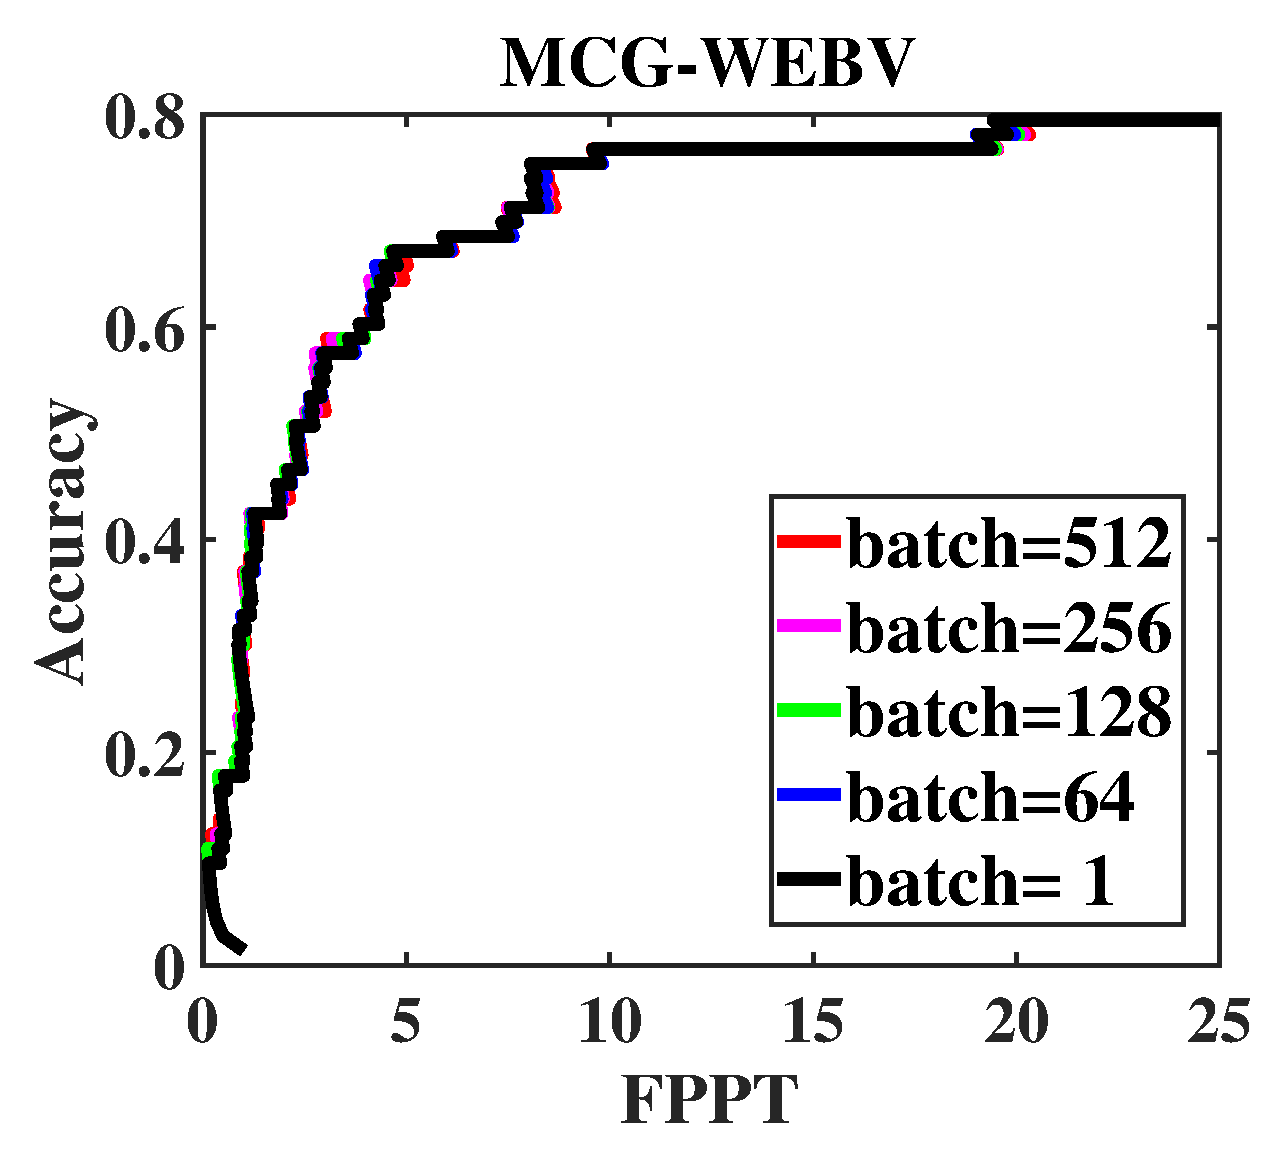
\includegraphics[width=\textwidth,height=0.95\textwidth]{minibatch_Accuracy}
      \caption{}
      \label{fig:minibatch_Accuracy}
    \end{subfigure}%
    % ~% add desired spacing
    \begin{subfigure}[b]{0.5\textwidth}
      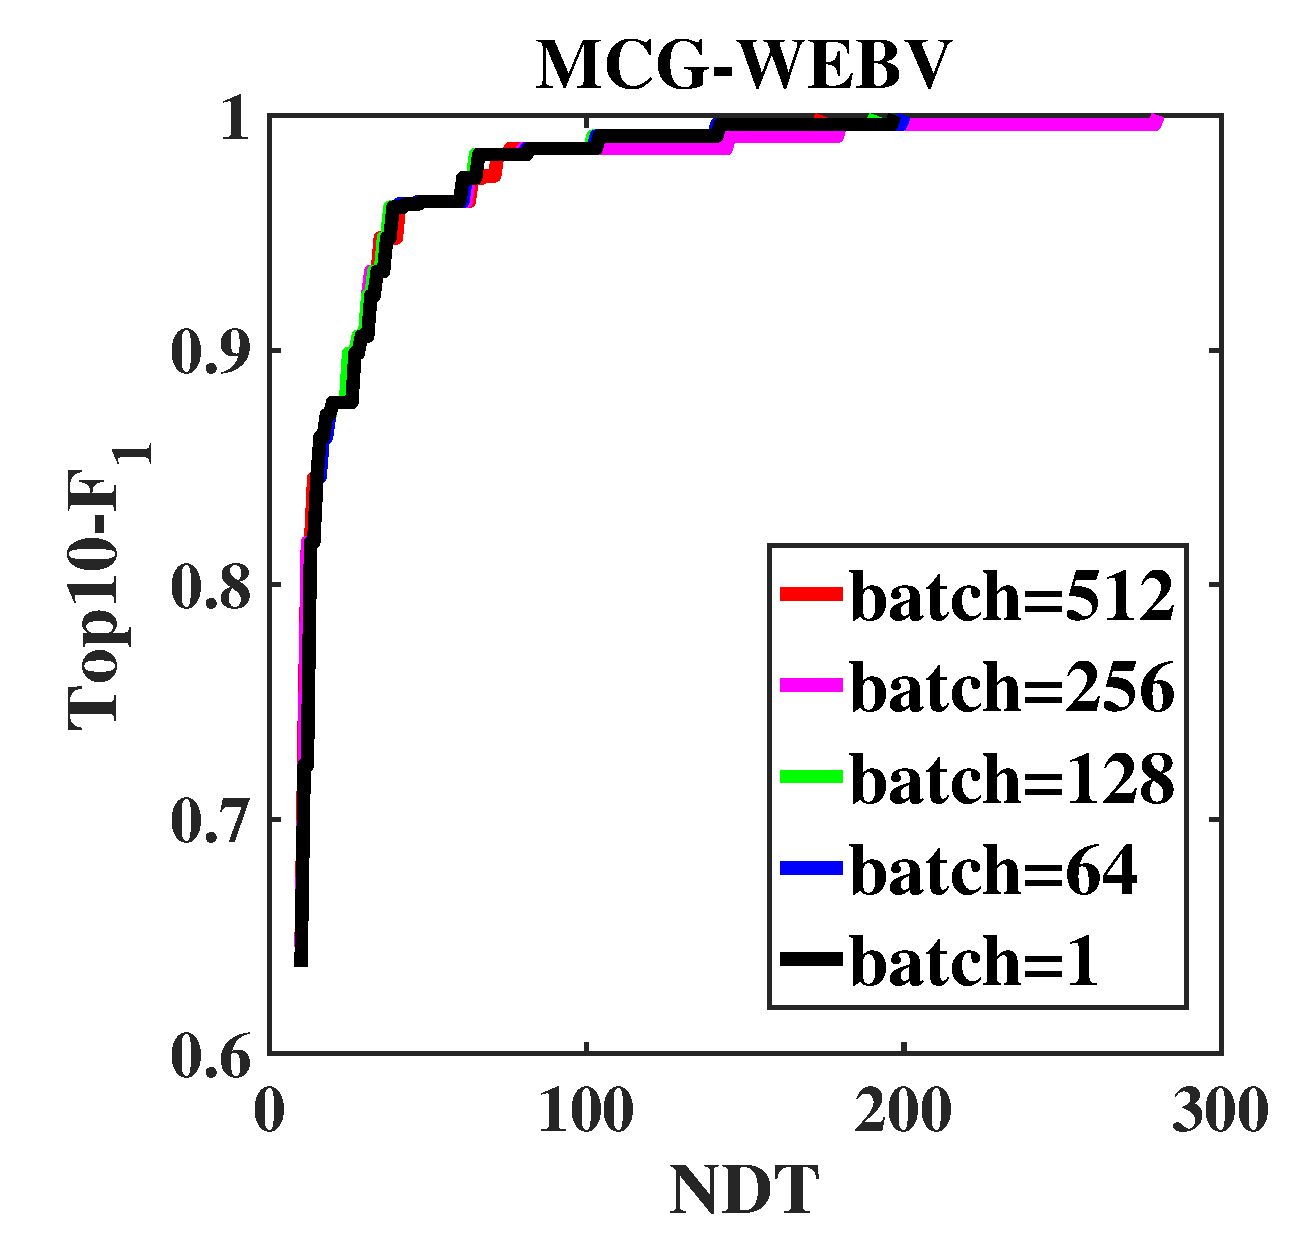
\includegraphics[width=\textwidth,height=0.95\textwidth]{minibatch_Top10}
      \caption{}
      \label{fig:minibatch_Top10}
    \end{subfigure}
    \caption{不同批样本数量$b$的话题排序效果对比}
    \label{fig:minibatch-two-metric}
\end{figure}

\subsubsection{权重参数$\alpha$和$\beta$:}

我们在公式\eqref{eq:weightupdate}使用了一个衰减权重。其中$\beta$是一个初始权重,$\alpha$是一个权重衰减因子。

图\ref{fig:Objective_Beta}展示了当固定其他参数(比如:$\alpha=0$,$b=128$,$T=30$),不同$\beta$值在收敛速度上的对比。正如所预期的那样,$\beta$越大,SPD算法的收敛速度越快。这是因为一个较大的$\beta$值使得近似代理函数能够快速适应当前最新的代理函数。
\begin{figure}[!htbp]
    \centering
    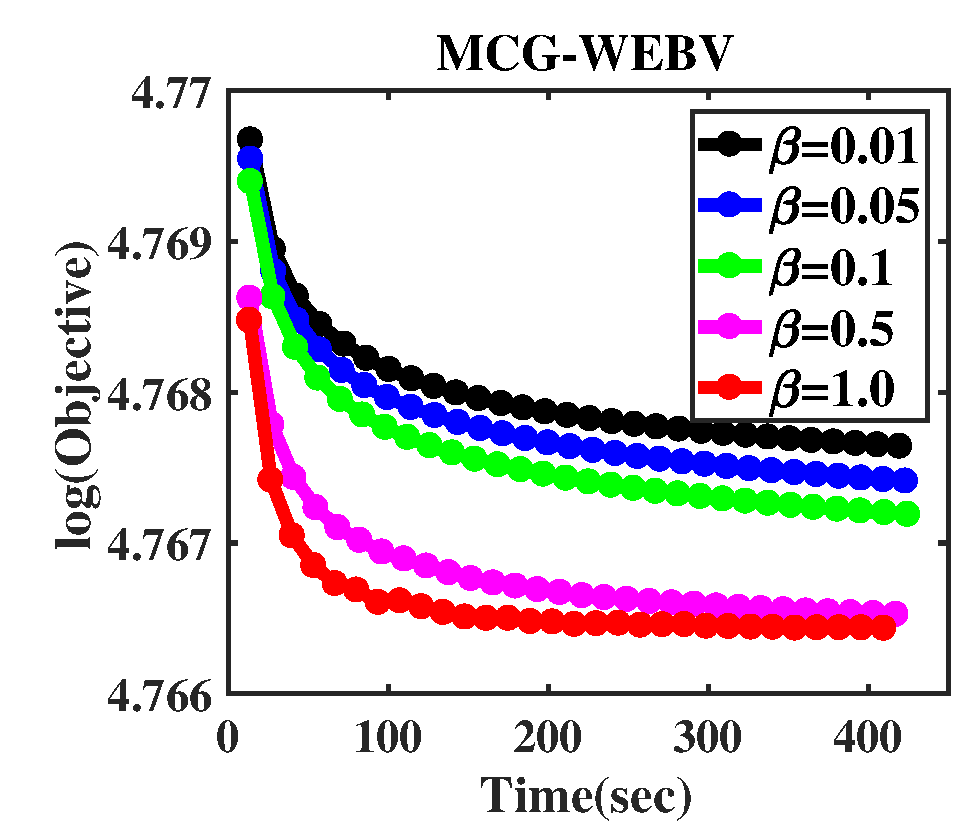
\includegraphics[width=0.7\textwidth]{Objective_Beta}
    \caption{不同$\beta$值对目标函数收敛曲线的影响}
    \label{fig:Objective_Beta}
\end{figure}

从图\ref{fig:differentbeta}的结果中,我们发现一个较大的$\beta$值不仅会带来更快的收敛速度,而且也会带来更好的话题排序效果。
\begin{figure}[!htbp]
    \centering
    \begin{subfigure}[b]{0.5\textwidth}
      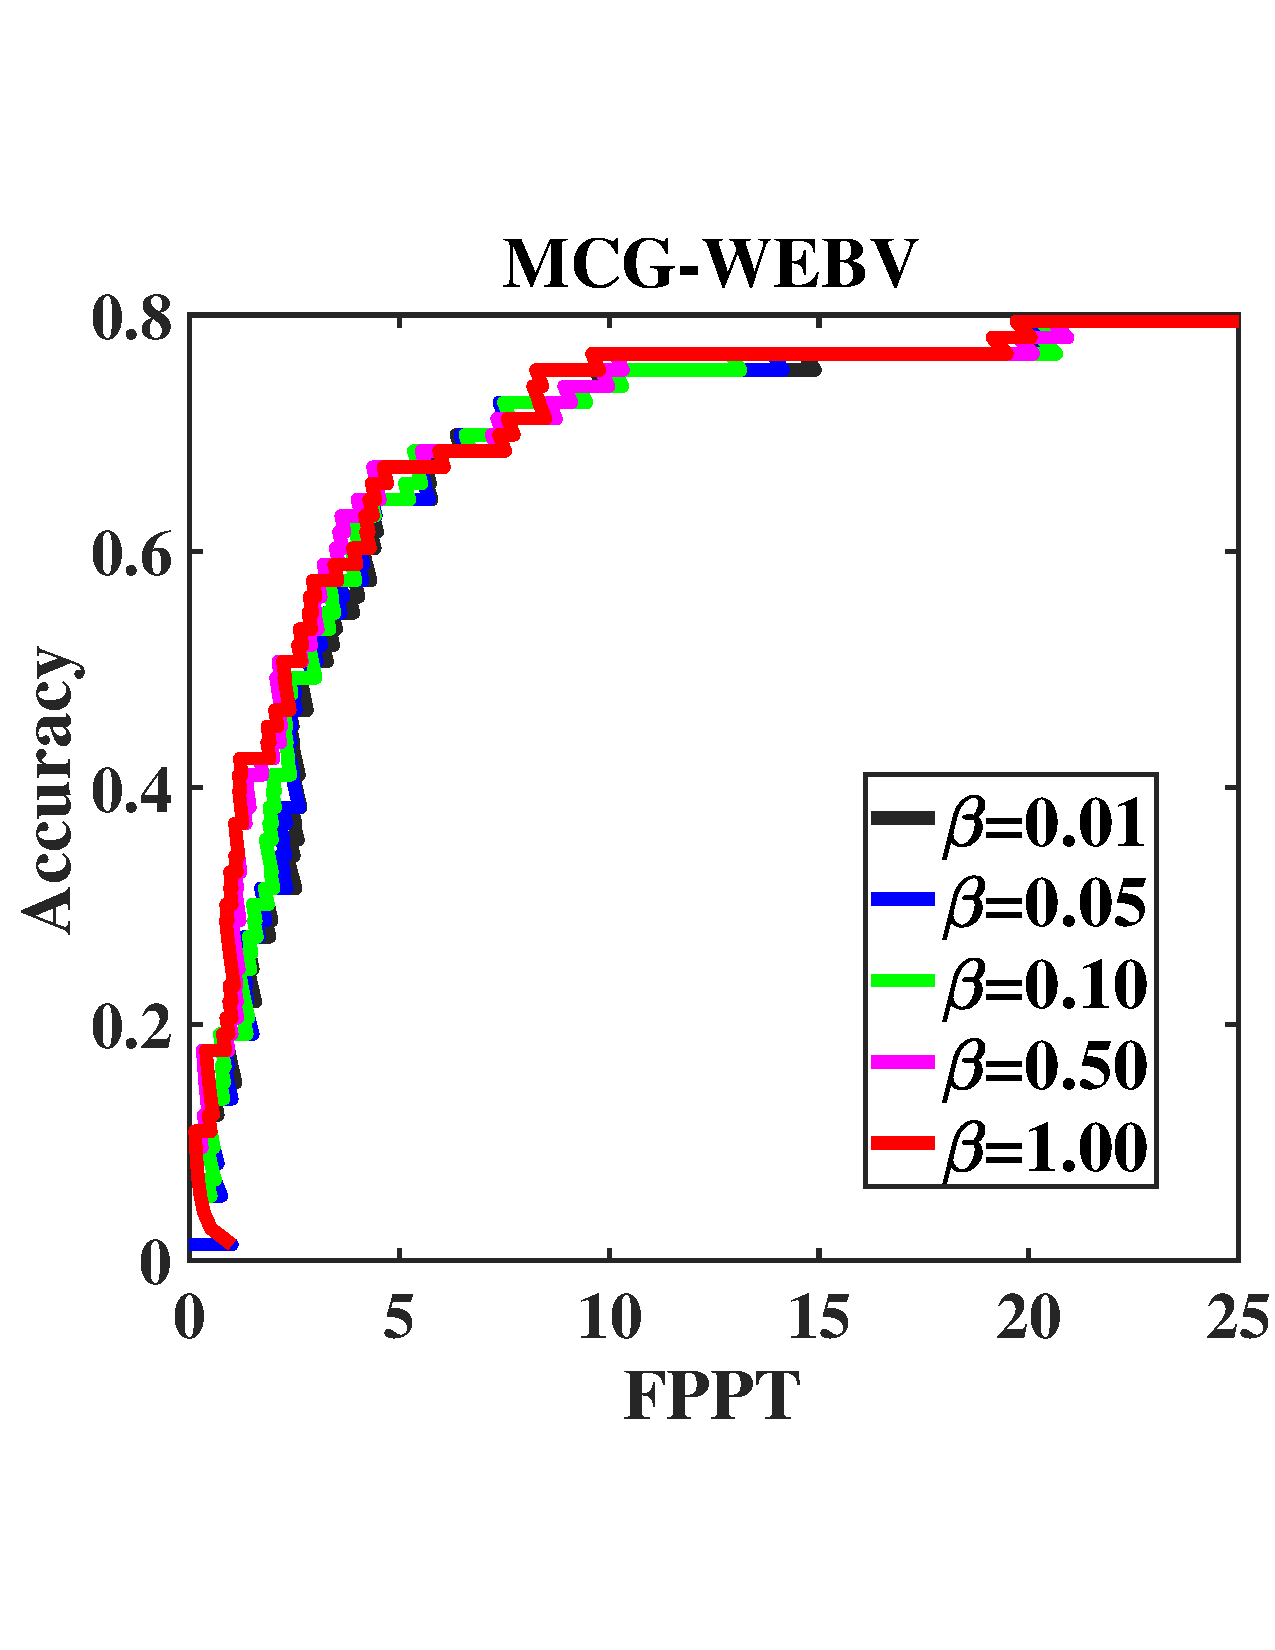
\includegraphics[width=\textwidth,height=0.95\textwidth]{Accuracy_Beta}
      \caption{}
      \label{fig:Accuracy_Beta}
    \end{subfigure}%
    % ~% add desired spacing
    \begin{subfigure}[b]{0.5\textwidth}
      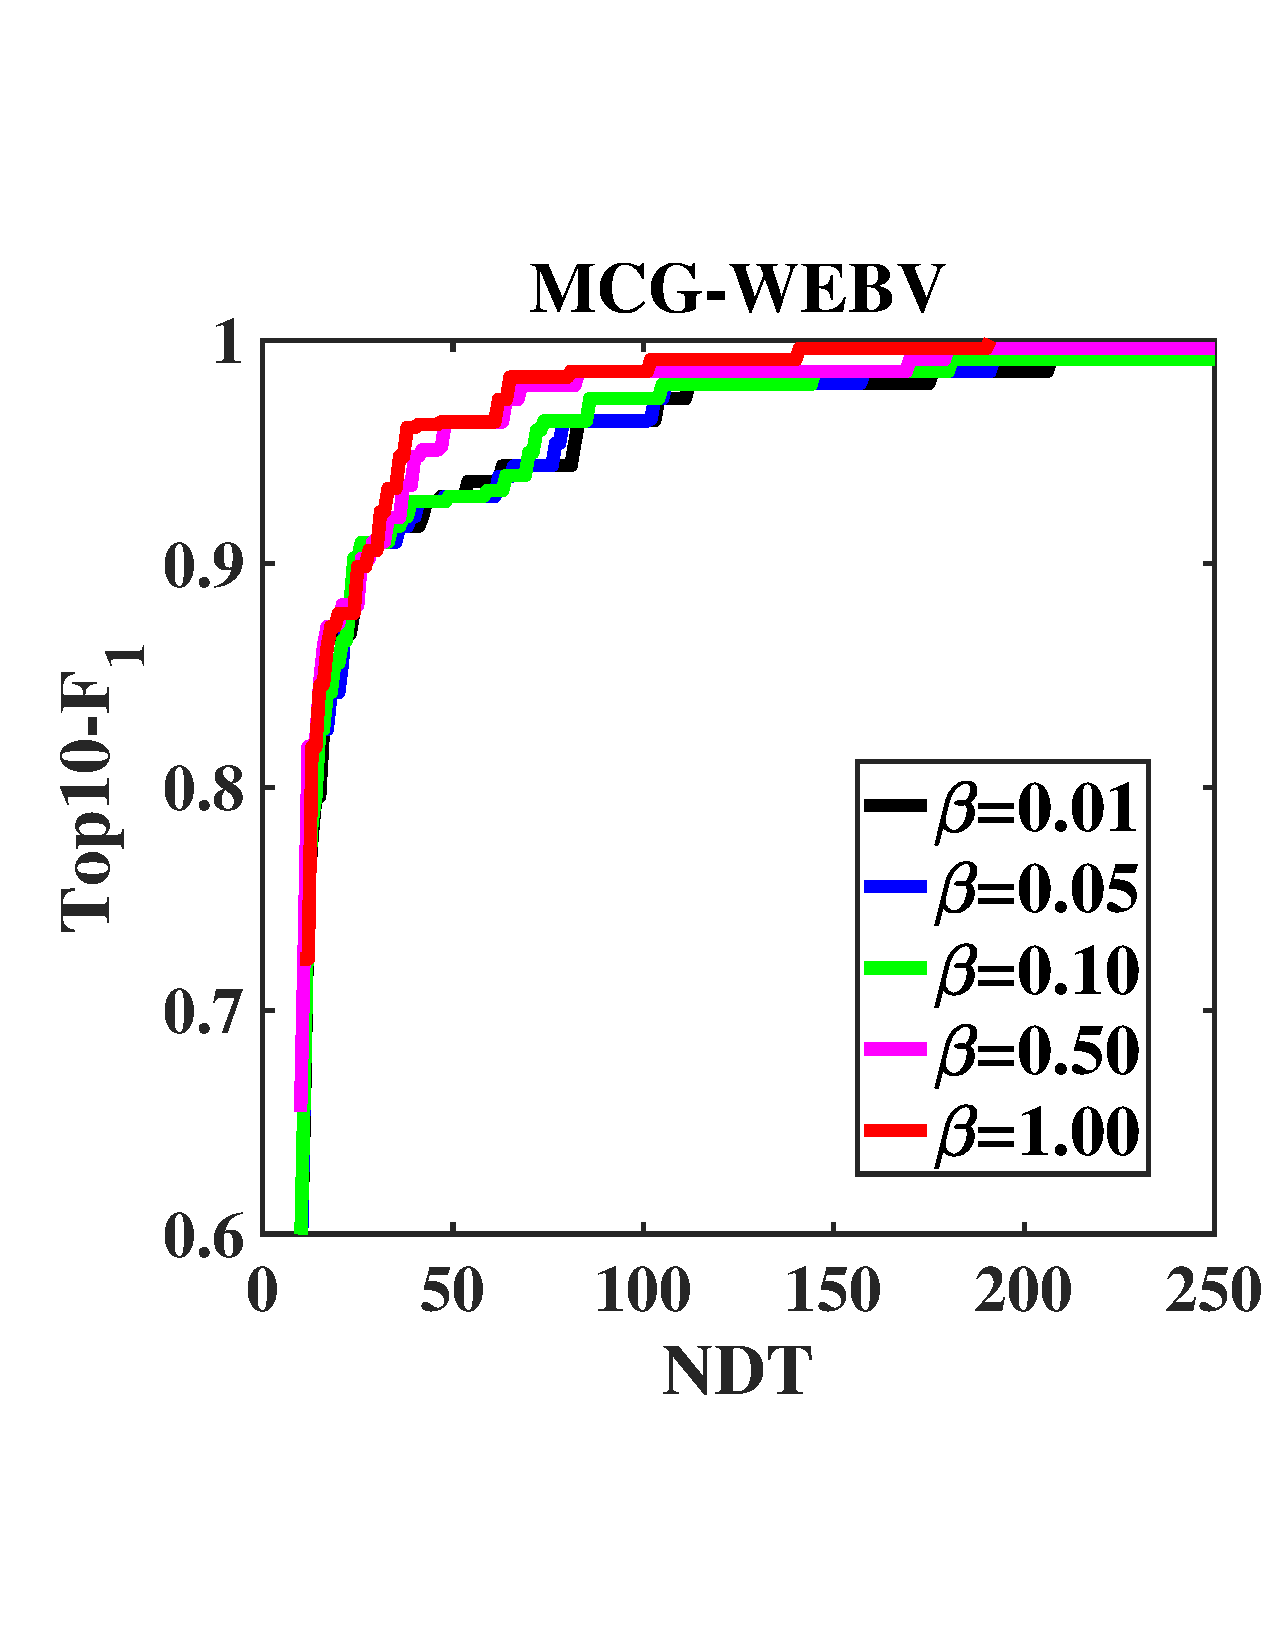
\includegraphics[width=\textwidth,height=0.95\textwidth]{Top10_Beta}
      \caption{}
      \label{fig:Top10_Beta}
    \end{subfigure}
    \caption{不同$\beta$值的话题排序效果对比}
    \label{fig:differentbeta}
\end{figure}

图\ref{fig:Objective_Alpha}展示了当固定其他参数(比如:$\beta=1$,$b=128$,$T=30$),不同$\alpha$值在收敛速度上的对比。从图中可以看出一个更小的$\alpha$会带来一个更平滑的目标函数收敛曲线。这是因为更小的$\alpha$值不仅使得$\beta$值衰减更快,而且也会使得SPD算法对于当前样本带来的代理函数更加的稳定。虽然不同$\alpha$值的收敛过程不太一样,但是最终都会收敛到一个相似的局部极小值。
\begin{figure}[!htbp]
    \centering
    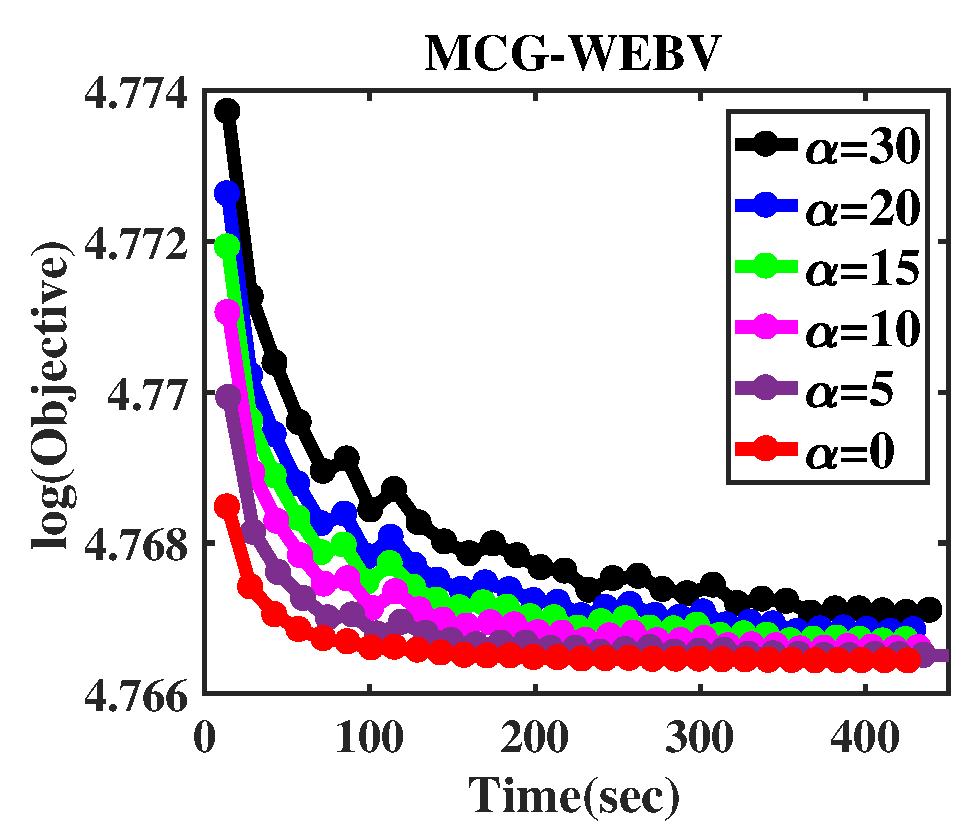
\includegraphics[width=0.7\textwidth]{Objective_Alpha}
    \caption{不同$\alpha$值对目标函数收敛曲线的影响}
    \label{fig:Objective_Alpha}
\end{figure}

从图\ref{fig:differentalpha}的结果中,可以看出不同$\alpha$值的话题排序性能几乎是一致的。
\begin{figure}[!htbp]
    \centering
    \begin{subfigure}[b]{0.5\textwidth}
      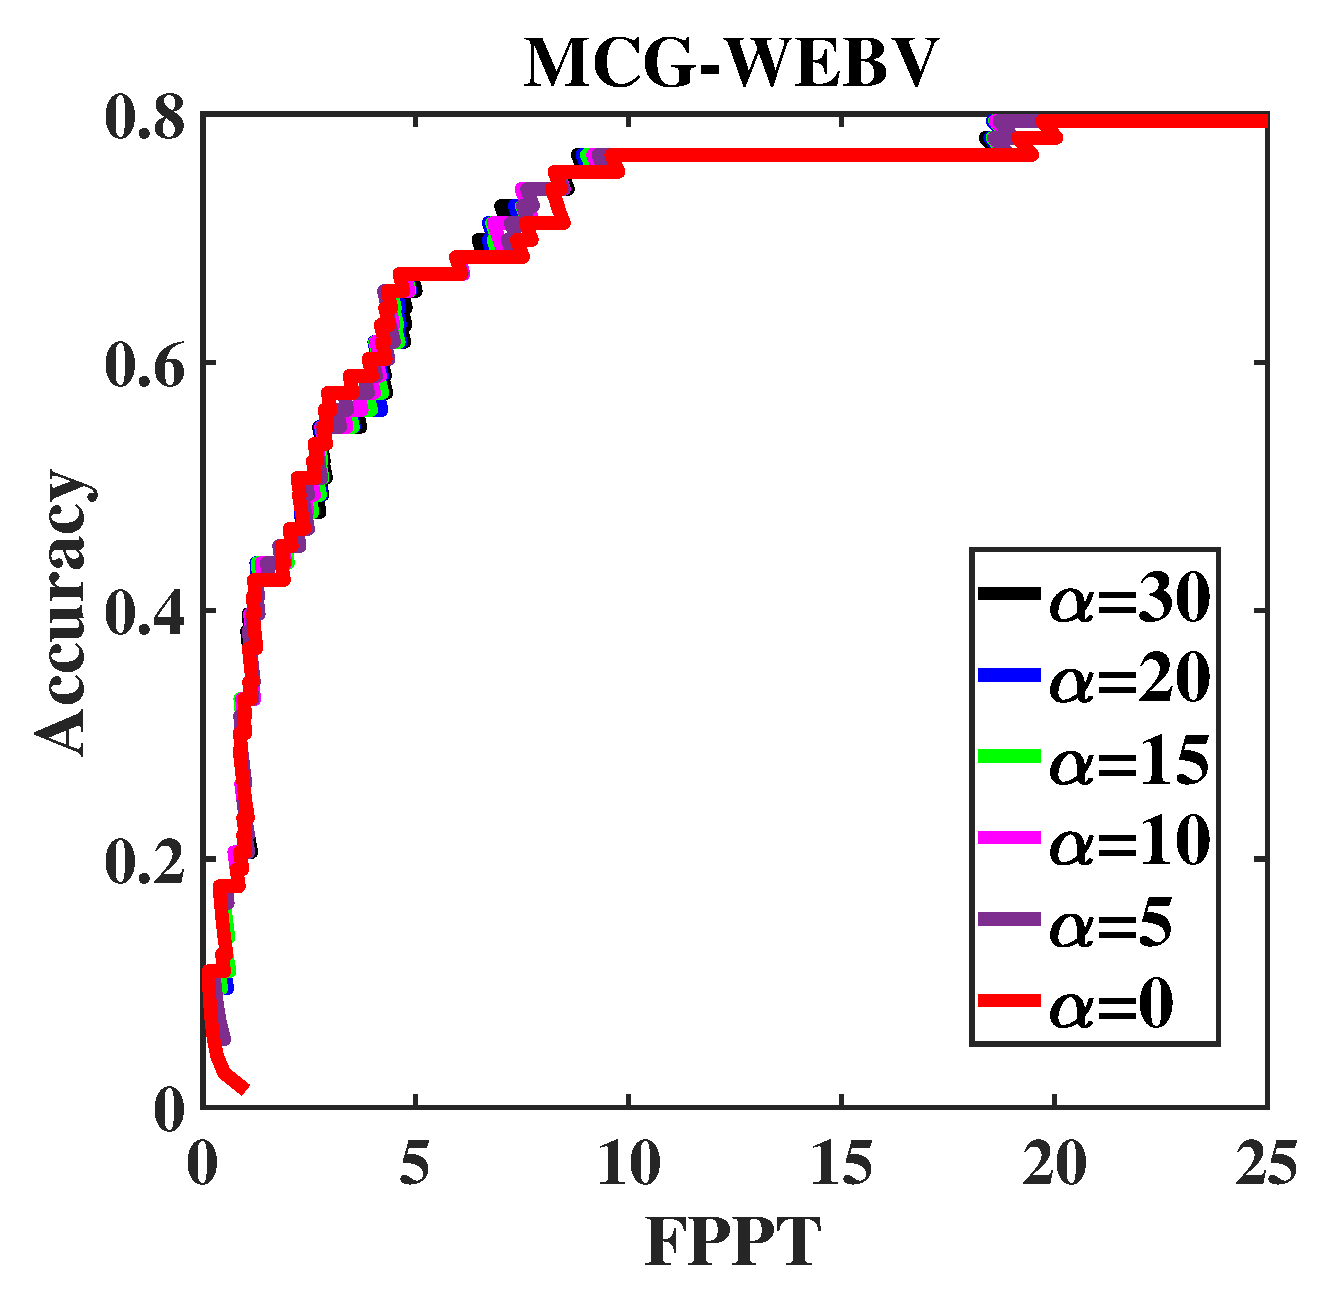
\includegraphics[width=\textwidth,height=0.95\textwidth]{Accuracy_Alpha}
      \caption{}
      \label{fig:Accuracy_Alpha}
    \end{subfigure}%
    % ~% add desired spacing
    \begin{subfigure}[b]{0.5\textwidth}
      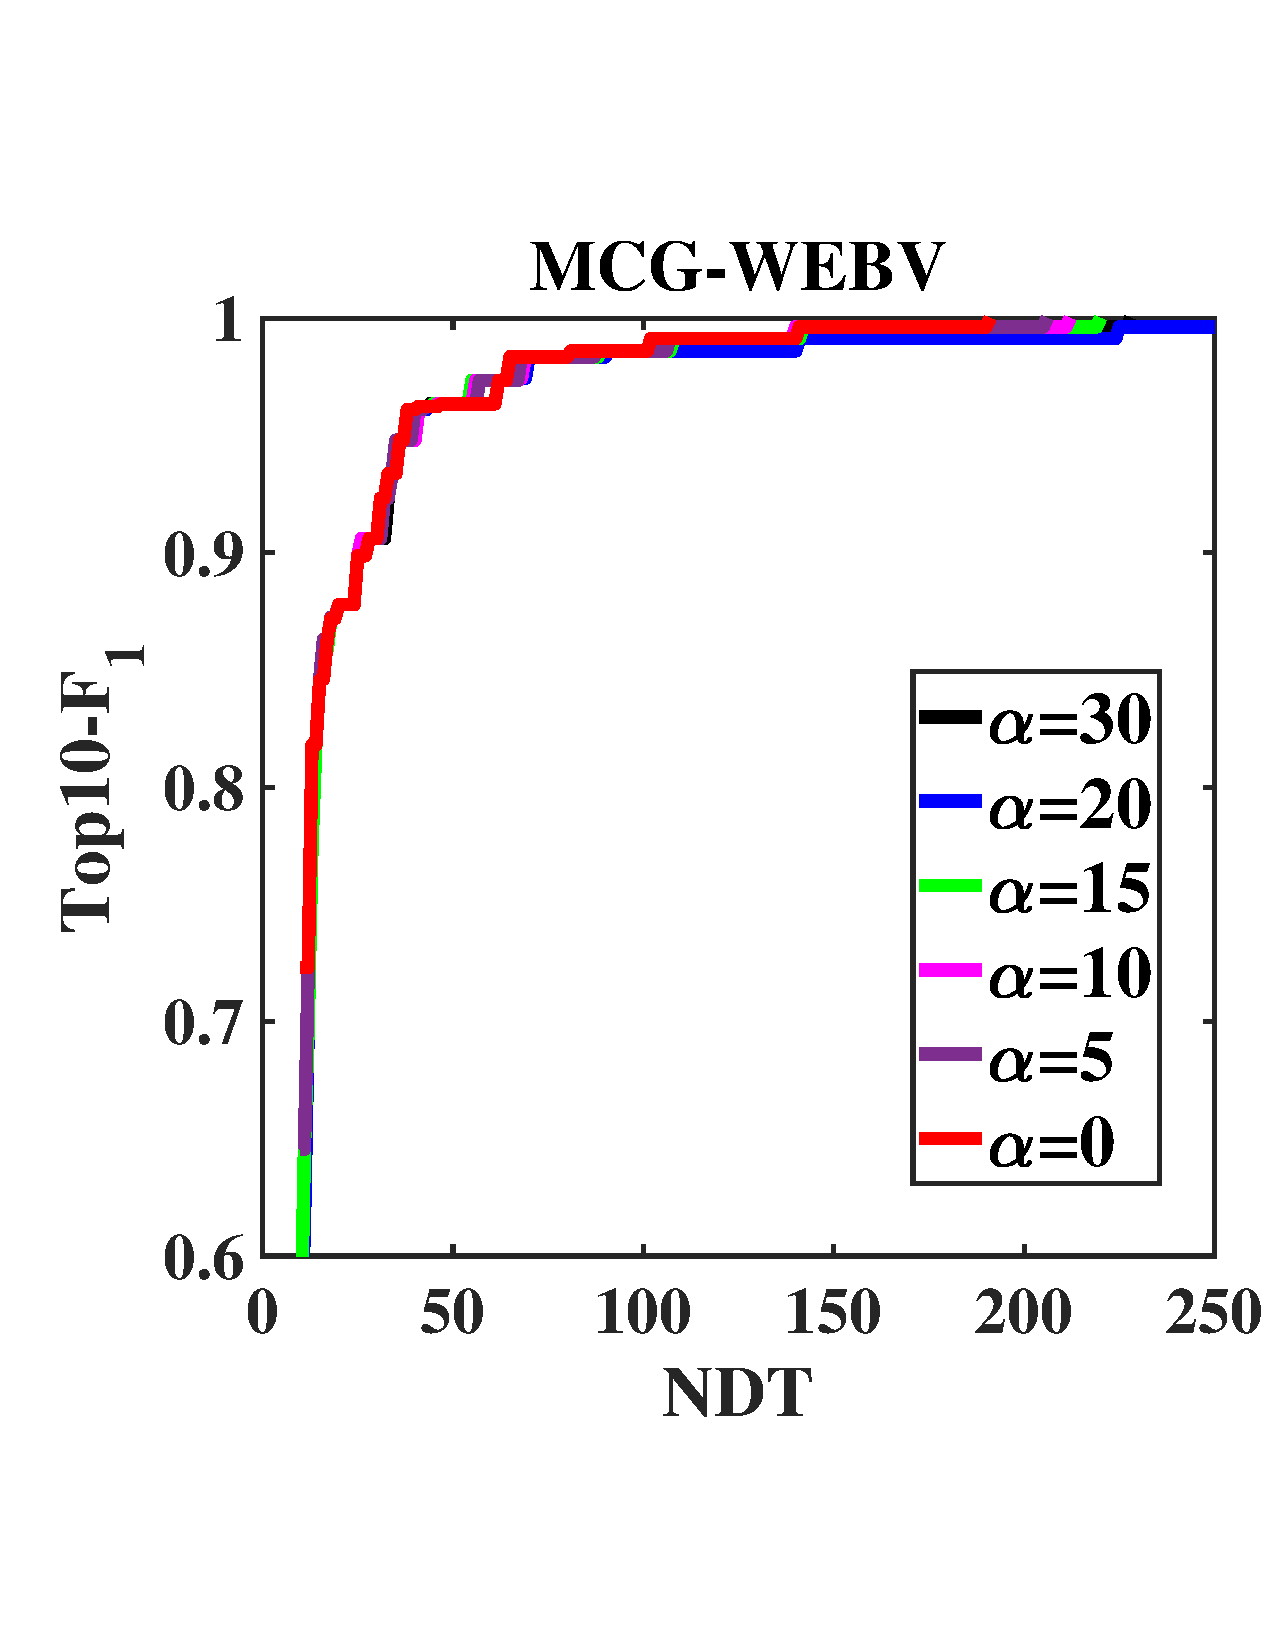
\includegraphics[width=\textwidth,height=0.95\textwidth]{Top10_Alpha}
      \caption{}
      \label{fig:Top10_Alpha}
    \end{subfigure}
    \caption{不同$\alpha$值的话题排序效果对比}
    \label{fig:differentalpha}
\end{figure}

通过以上实验结果可以得到,不同的$\alpha$和$\beta$值虽然会在一定程度上影响SPD算法中目标函数的收敛速度,但是从$Accuracy$和Top10-$F_1$来看,这些不同参数的不同取值对话题排序效果的影响不是很大。所以,可以认为我们的SPD算法是一个对参数具有鲁棒性的算法。


\subsection{异步并行实验}

我们使用python语言开了4个进程来实现AsySPD算法。图\ref{fig:ToyData_Objective_AsySPD}展示了SPD算法和AsySPD算法在人工数据集上的收敛情况。从图中可以看出,AsySPD算法相对SPD算法的加速比达到了3.3倍,证明AsySPD算法是有效的。但是AsySPD算法的收敛值比SPD算法大,这可能是因为使用了异步无锁并行策略,导致在使用相同数量样本进行更新时,样本利用率不高,且存在更新冲突,从而收敛到一个较大的局部极小值。
\begin{figure}[!htbp]
    \centering
    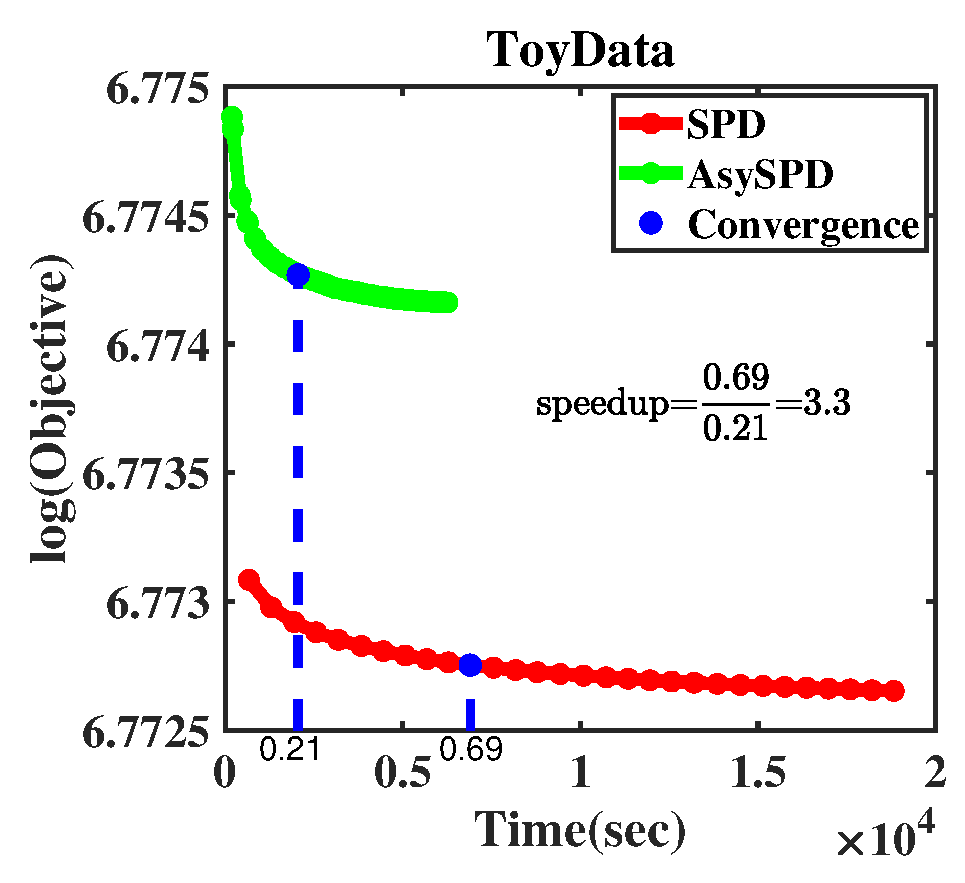
\includegraphics[width=0.7\textwidth]{ToyData_Objective_Asy}
    \caption{SPD和AsySPD算法在ToyData上的收敛对比}
    \label{fig:ToyData_Objective_AsySPD}
\end{figure}

图\ref{fig:MCG_YKS_Objective_AsySPD}展示了SPD算法和AsySPD算法在MCG-WEBV和YKS数据集上的收敛情况。同样发现AsySPD相比SPD收敛到一个较大的局部极小值。AsySPD算法的收敛趋势比较接近PD算法。
\begin{figure}[!htbp]
    \centering
    \begin{subfigure}[b]{0.5\textwidth}
      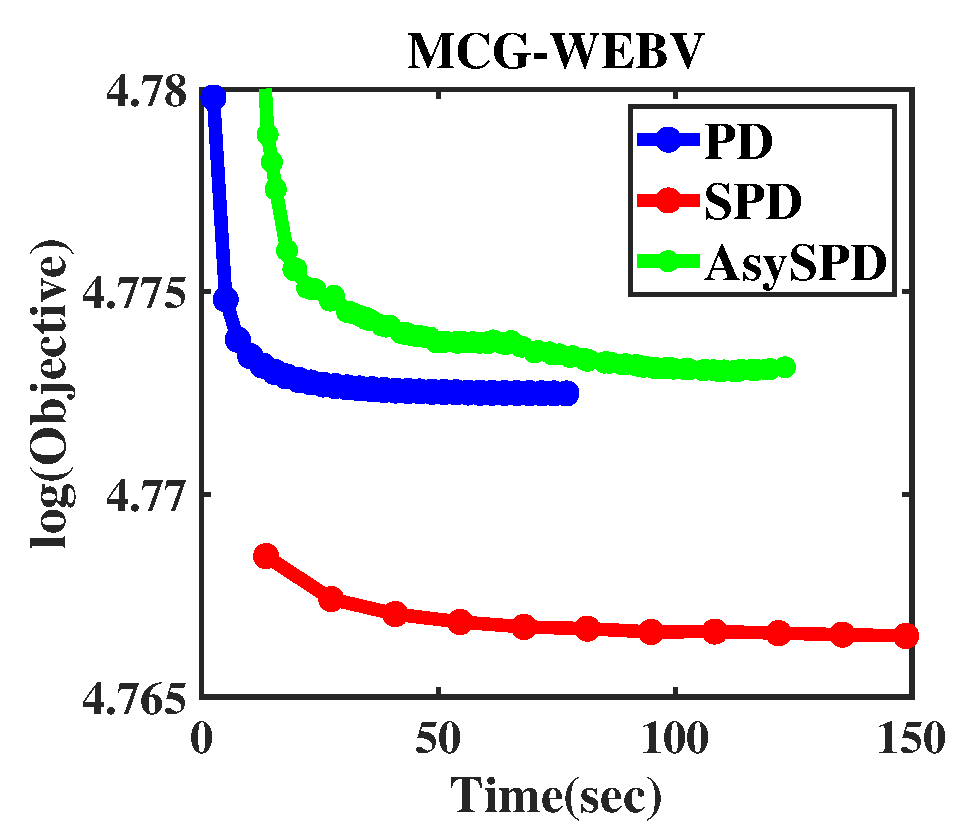
\includegraphics[width=\textwidth,height=0.95\textwidth]{MCG_Objective_Asy}
      \caption{}
      \label{fig:MCG_Objective_Asy}
    \end{subfigure}%
    % ~% add desired spacing
    \begin{subfigure}[b]{0.5\textwidth}
      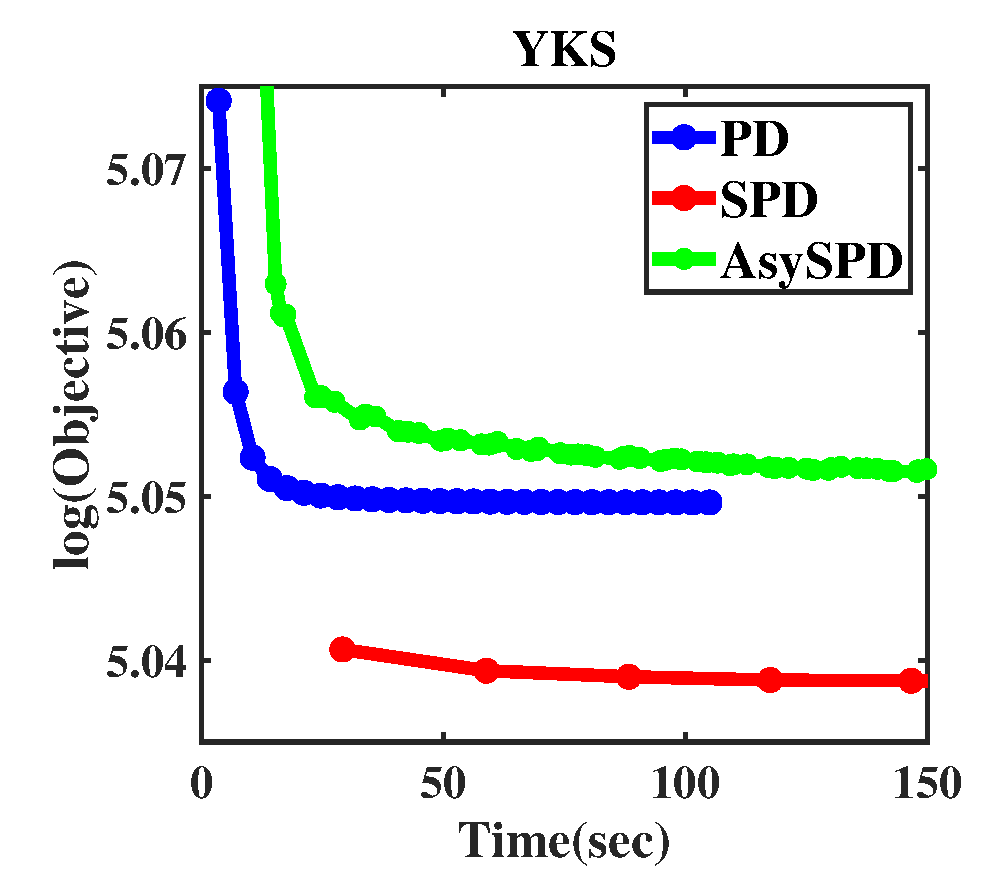
\includegraphics[width=\textwidth,height=0.95\textwidth]{YKS_Objective_Asy}
      \caption{}
      \label{fig:YKS_Objective_Asy}
    \end{subfigure}
    \caption{SPD和AsySPD算法在MCG-WEBV和YKS数据集上的收敛对比}
    \label{fig:MCG_YKS_Objective_AsySPD}
\end{figure}

\begin{figure}[!htbp]
    \centering
    \begin{subfigure}[b]{0.5\textwidth}
      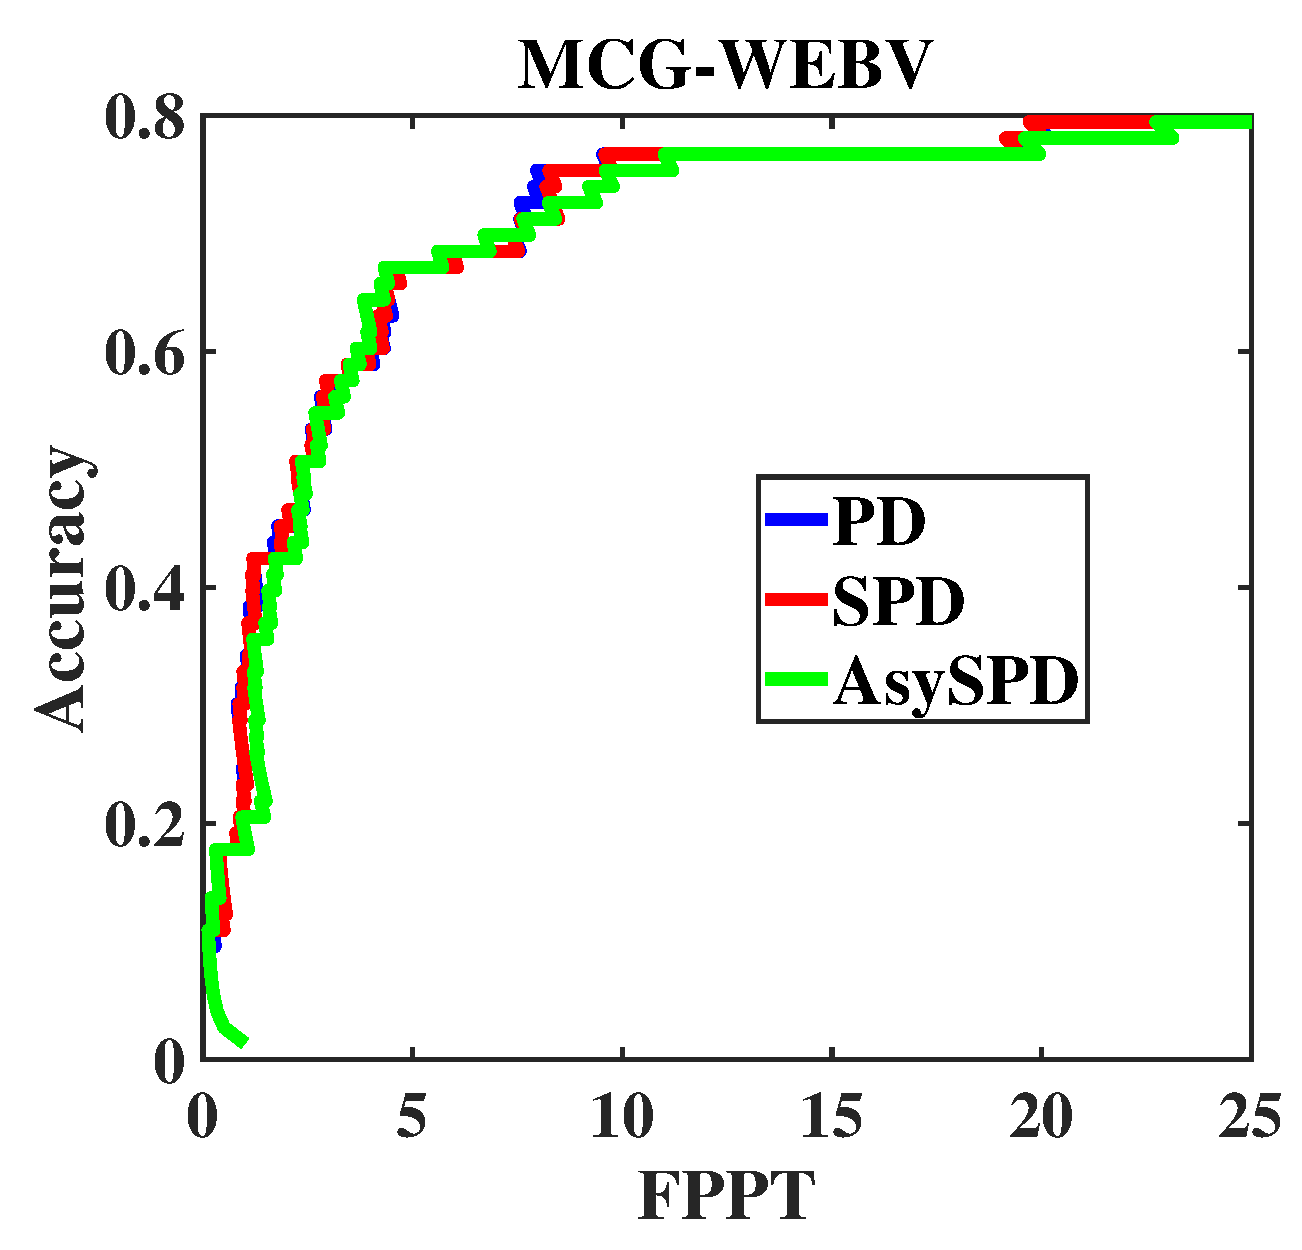
\includegraphics[width=\textwidth,height=0.95\textwidth]{MCG_Accuracy_Asy}
      \caption{}
      \label{fig:MCG_Accuracy_Asy}
    \end{subfigure}%
    % ~% add desired spacing
    \begin{subfigure}[b]{0.5\textwidth}
      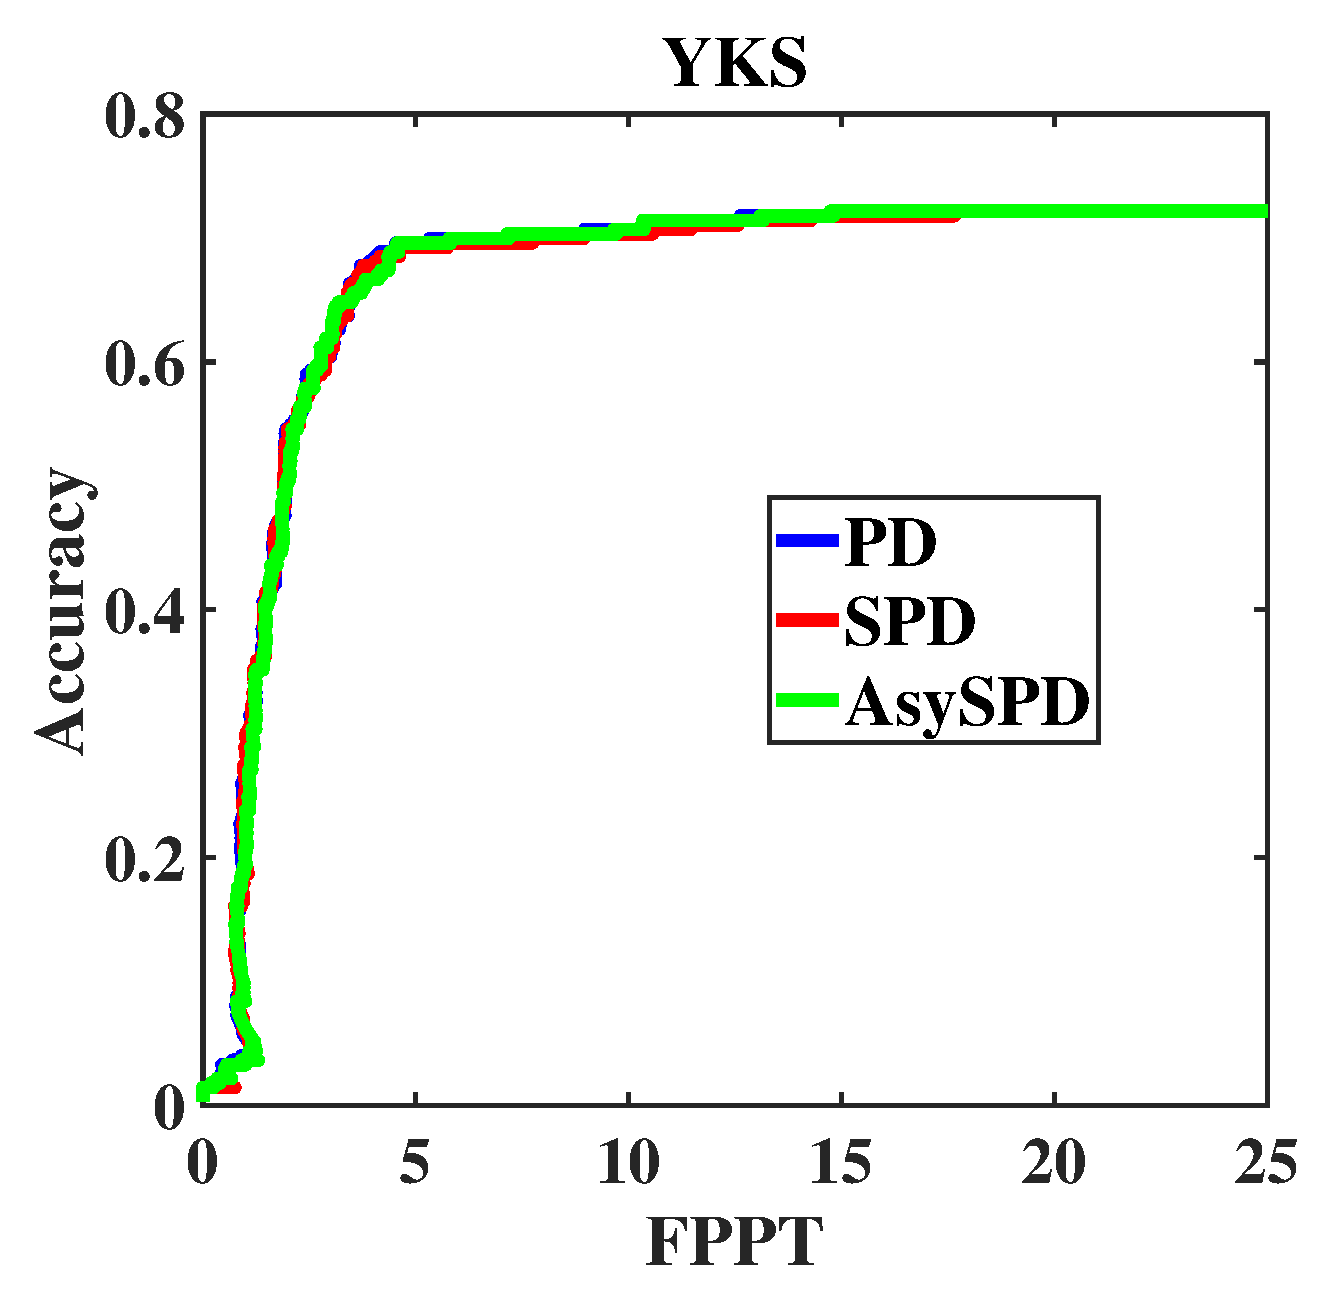
\includegraphics[width=\textwidth,height=0.95\textwidth]{YKS_Accuracy_Asy}
      \caption{}
      \label{fig:YKS_Accuracy_Asy}
    \end{subfigure}
    \caption{使用$Accuracy$ v.s. $FPPT$对比SPD和AsySPD算法}
    \label{fig:MCG_YKS_Accuracy_AsySPD}
\end{figure}
最后,我们在MCG-WEBV和YKS数据集上对比这两个算法的话题排序效果。从图\ref{fig:MCG_YKS_Accuracy_AsySPD}可以看出AsySPD算法与SPD算法在$Accuracy$上的排序上效果一致。从图\ref{fig:MCG_YKS_Top10_AsySPD}可以看出这两个算法在Top10-$F_1$的排序上效果也几乎一致。综上,实际数据集的实验结果可以经验地证明我们AsySPD算法的有效性和高效性。
\begin{figure}[!htbp]
    \centering
    \begin{subfigure}[b]{0.5\textwidth}
      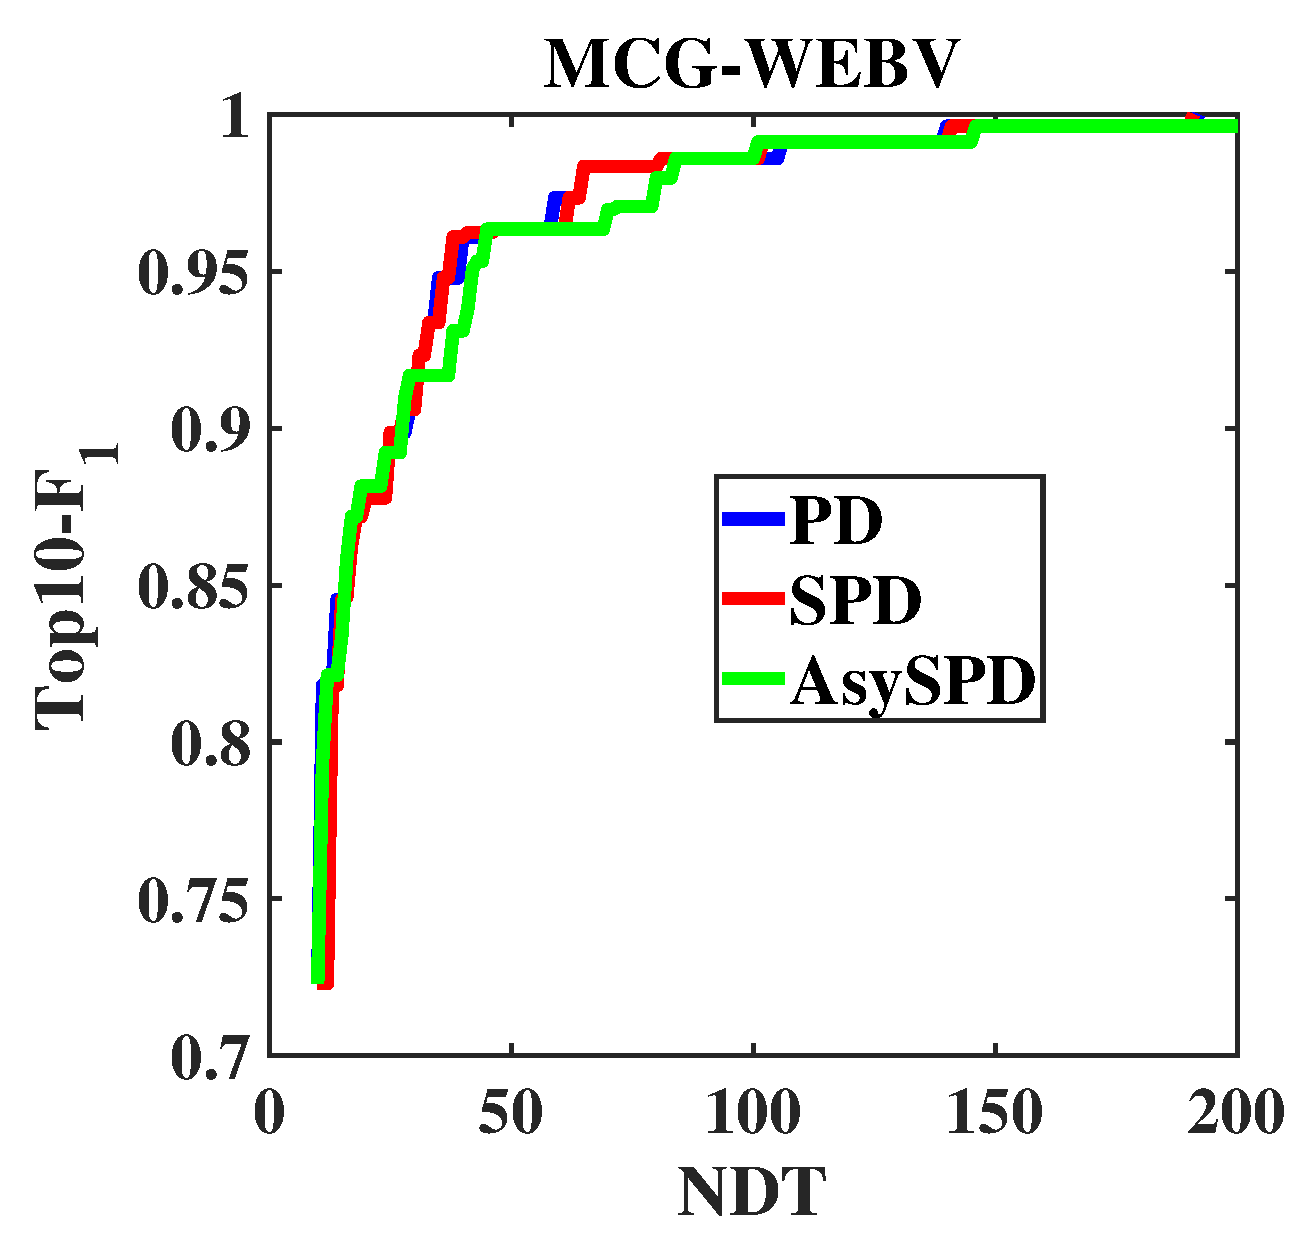
\includegraphics[width=\textwidth,height=0.95\textwidth]{MCG_Top10_Asy}
      \caption{}
      \label{fig:MCG_Top10_Asy}
    \end{subfigure}%
    % ~% add desired spacing
    \begin{subfigure}[b]{0.5\textwidth}
      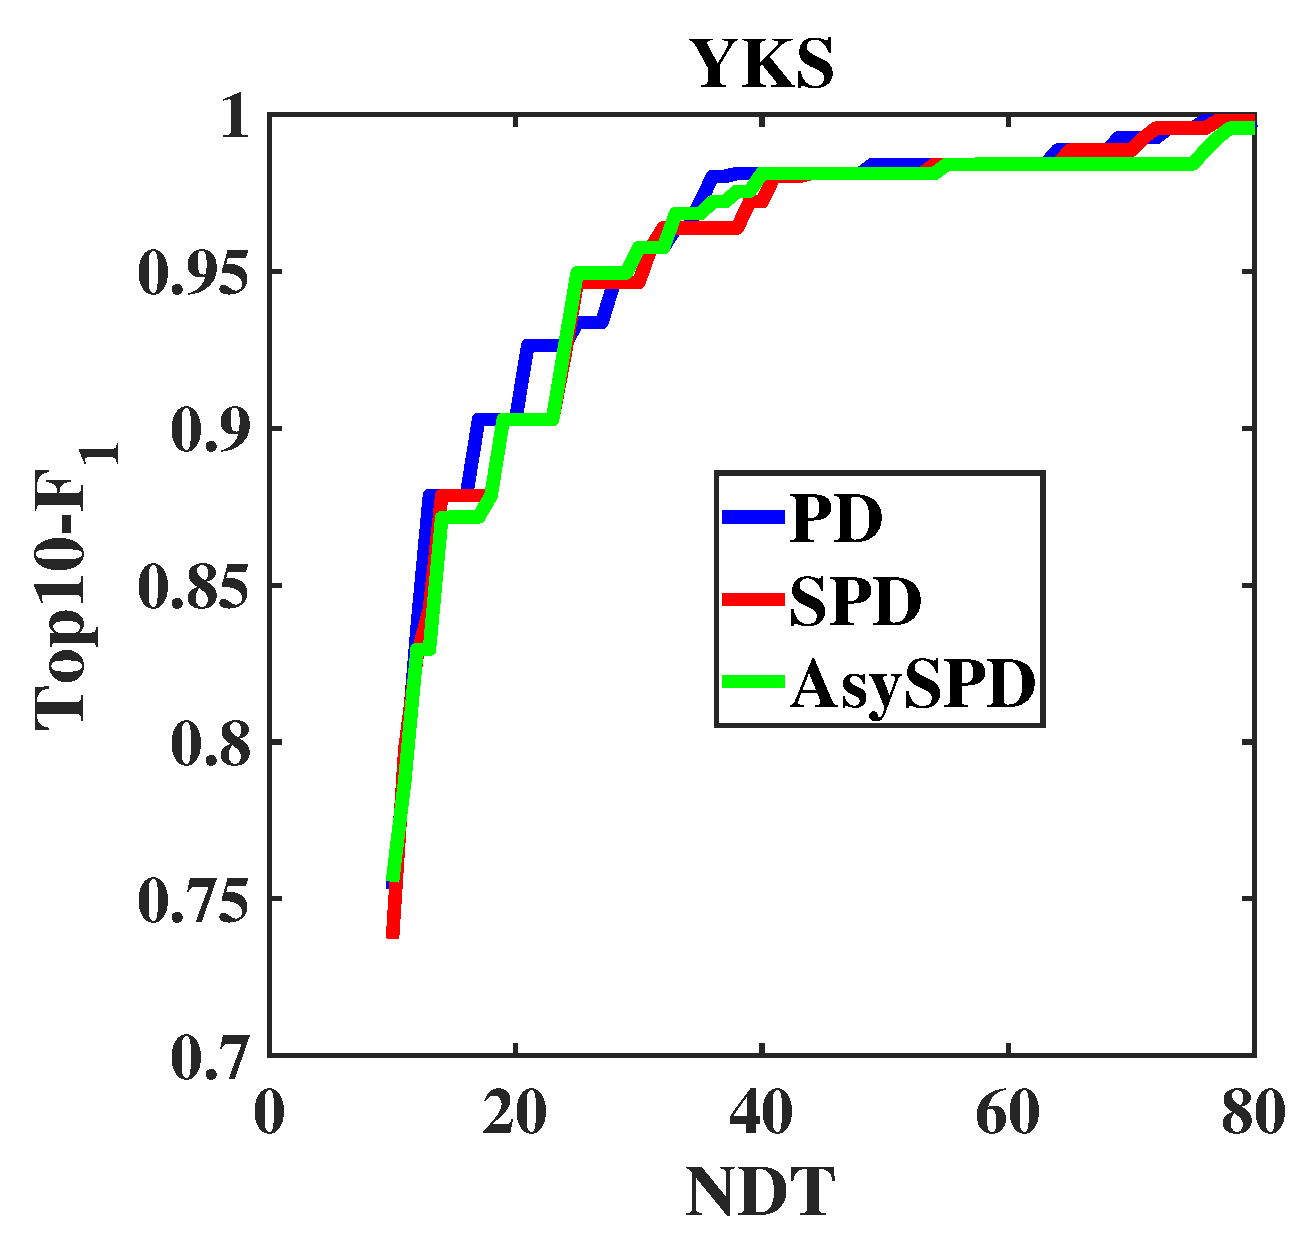
\includegraphics[width=\textwidth,height=0.95\textwidth]{YKS_Top10_Asy}
      \caption{}
      \label{fig:YKS_Top10_Asy}
    \end{subfigure}
    \caption{使用Top10-$F_1$ v.s. $NDT$对比SPD和AsySPD算法}
    \label{fig:MCG_YKS_Top10_AsySPD}
\end{figure}



\section{小结}

在本章中,我们提出了一种SPD算法,将随机优化最小化原则应用到PD算法中,从而能够优雅地处理大规模网络数据的话题检测问题。SPD算法迭代的利用小批量样本来更新目标函数的上界代理函数,同时最小化该代理函数,从而单调地驱使目标函数值下降。应用过程中注意到话题检测的特殊场景:一小批样本只能更新一部分话题的权重,而传统的随机梯度下降中的小批量样本能更新所有的权重。所以,在每次更新时,只更新那些被当前批样本影响到的话题。最终在话题检测效果方面,我们通过实验展示了我们的算法可以取得和当前最好的话题检测算法相似的性能。同时,我们构造了一个较大规模的人工数据集来验证我们算法高效的收敛速度。最后,我们提出AsySPD算法来实现SPD算法的异步并行更新。
\chapter{总结与展望}\label{chap:ConclusionProspect.tex}

\section{本文工作总结}


\section{未来研究展望}


%---------------------------------------------------------------------------%
% main content
%-
%-> Appendix
%-
\cleardoublepage%
\appendix% initialize the environment
% \chapter{中国科学院大学学位论文撰写要求}

学位论文是研究生科研工作成果的集中体现,是评判学位申请者学术水平、授予其学位的主要依据,是科研领域重要的文献资料。根据《科学技术报告、学位论文和学术论文的编写格式》(GB/T 7713-1987)、《学位论文编写规则》(GB/T 7713.1-2006)和《文后参考文献著录规则》(GB7714—87)等国家有关标准,结合中国科学院大学(以下简称“国科大”)的实际情况,特制订本规定。

\section{论文无附录者无需附录部分}

\section{测试公式编号} \label{sec:testmath}

\begin{equation} \label{eq:appedns}
    \adddotsbeforeeqnnum%
    \begin{cases}
        \frac{\partial \rho}{\partial t} + \nabla\cdot(\rho\Vector{V}) = 0\\
        \frac{\partial (\rho\Vector{V})}{\partial t} + \nabla\cdot(\rho\Vector{V}\Vector{V}) = \nabla\cdot\Tensor{\sigma}\\
        \frac{\partial (\rho E)}{\partial t} + \nabla\cdot(\rho E\Vector{V}) = \nabla\cdot(k\nabla T) + \nabla\cdot(\Tensor{\sigma}\cdot\Vector{V})
    \end{cases}
\end{equation}
\begin{equation}
    \adddotsbeforeeqnnum%
    \frac{\partial }{\partial t}\int\limits_{\Omega} u \, \mathrm{d}\Omega + \int\limits_{S} \unitVector{n}\cdot(u\Vector{V}) \, \mathrm{d}S = \dot{\phi}
\end{equation}

\section{测试生僻字}

霜蟾盥薇曜灵霜颸妙鬘虚霩淩澌菀枯菡萏泬寥窅冥毰毸濩落霅霅便嬛岧峣瀺灂姽婳愔嫕飒纚棽俪緸冤莩甲摛藻卮言倥侗椒觞期颐夜阑彬蔚倥偬澄廓簪缨陟遐迤逦缥缃鹣鲽憯懔闺闼璀错媕婀噌吰澒洞阛闠覼缕玓瓑逡巡諓諓琭琭瀌瀌踽踽叆叇氤氲瓠犀流眄蹀躞赟嬛茕頔璎珞螓首蘅皋惏悷缱绻昶皴皱颟顸愀然菡萏卑陬纯懿犇麤掱暒 墌墍墎墏墐墒墒墓墔墕墖墘墖墚墛坠墝增墠墡墢墣墤墥墦墧墨墩墪樽墬墭堕墯墰墱墲坟墴墵垯墷墸墹墺墙墼墽垦墿壀壁壂壃壄壅壆坛壈壉壊垱壌壍埙壏壐壑壒压壔壕壖壗垒圹垆壛壜壝垄壠壡坜壣壤壥壦壧壨坝塆圭嫶嫷嫸嫹嫺娴嫼嫽嫾婳妫嬁嬂嬃嬄嬅嬆嬇娆嬉嬊娇嬍嬎嬏嬐嬑嬒嬓嬔嬕嬖嬗嬘嫱嬚嬛嬜嬞嬟嬠嫒嬢嬣嬥嬦嬧嬨嬩嫔嬫嬬奶嬬嬮嬯婴嬱嬲嬳嬴嬵嬶嬷婶嬹嬺嬻嬼嬽嬾嬿孀孁孂娘孄孅孆孇孆孈孉孊娈孋孊孍孎孏嫫婿媚嵭嵮嵯嵰嵱嵲嵳嵴嵵嵶嵷嵸嵹嵺嵻嵼嵽嵾嵿嶀嵝嶂嶃崭嶅嶆岖嶈嶉嶊嶋嶌嶍嶎嶏嶐嶑嶒嶓嵚嶕嶖嶘嶙嶚嶛嶜嶝嶞嶟峤嶡峣嶣嶤嶥嶦峄峃嶩嶪嶫嶬嶭崄嶯嶰嶱嶲嶳岙嶵嶶嶷嵘嶹岭嶻屿岳帋巀巁巂巃巄巅巆巇巈巉巊岿巌巍巎巏巐巑峦巓巅巕岩巗巘巙巚帠帡帢帣帤帨帩帪帬帯帰帱帲帴帵帷帹帺帻帼帽帾帿幁幂帏幄幅幆幇幈幉幊幋幌幍幎幏幐幑幒幓幖幙幚幛幜幝幞帜幠幡幢幤幥幦幧幨幩幪幭幮幯幰幱庍庎庑庖庘庛庝庠庡庢庣庤庥庨庩庪庬庮庯庰庱庲庳庴庵庹庺庻庼庽庿廀厕廃厩廅廆廇廋廌廍庼廏廐廑廒廔廕廖廗廘廙廛廜廞庑廤廥廦廧廨廭廮廯廰痈廲廵廸廹廻廼廽廿弁弅弆弇弉弖弙弚弜弝弞弡弢弣弤弨弩弪弫弬弭弮弰弲弪弴弶弸弻弼弽弿彖彗彘彚彛彜彝彞彟彴彵彶彷彸役彺彻彽彾佛徂徃徆徇徉后徍徎徏径徒従徔徕徖徙徚徛徜徝从徟徕御徢徣徤徥徦徧徨复循徫旁徭微徯徰徱徲徳徴徵徶德徸彻徺忁忂惔愔忇忈忉忔忕忖忚忛応忝忞忟忪挣挦挧挨挩挪挫挬挭挮挰掇授掉掊掋掍掎掐掑排掓掔掕挜掚挂掜掝掞掟掠采探掣掤掦措掫掬掭掮掯掰掱掲掳掴掵掶掸掹掺掻掼掽掾掿拣揁揂揃揅揄揆揇揈揉揊揋揌揍揎揑揓揔揕揖揗揘揙揤揥揦揧揨揫捂揰揱揲揳援揵揶揷揸揻揼揾揿搀搁搂搃搄搅搇搈搉搊搋搌搎搏搐搑搒摓摔摕摖摗摙摚摛掼摝摞摠摡斫斩斮斱斲斳斴斵斶斸旪旫旮旯晒晓晔晕晖晗晘晙晛晜晞晟晠晡晰晣晤晥晦晧晪晫晬晭晰晱晲晳晴晵晷晸晹晻晼晽晾晿暀暁暂暃暄暅暆暇晕晖暊暋暌暍暎暏暐暑暒暓暔暕暖暗旸暙暚暛暜暝暞暟暠暡暣暤暥暦暧暨暩暪暬暭暮暯暰昵暲暳暴暵暶暷暸暹暺暻暼暽暾暿曀曁曂曃晔曅曈曊曋曌曍曎曏曐曑曒曓曔曕曗曘曙曚曛曜曝曞曟旷曡曢曣曤曥曦曧昽曩曪曫晒曭曮曯椗椘椙椚椛検椝椞椟椠椡椢椣椤椥椦椧椨椩椪椫椬椭椮椯椰椱椲椳椴椵椶椷椸椹椺椻椼椽椾椿楀楁楂楃楅楆楇楈楉杨楋楌楍榴榵榶榷榸榹榺榻榼榽榾桤槀槁槂盘槄槅槆槇槈槉槊构槌枪槎槏槐槑槒杠槔槕槖槗滙滛滜滝滞滟滠滢滣滦滧滪滫沪滭滮滰滱渗滳滵滶滹滺浐滼滽漀漃漄漅漈漉溇漋漌漍漎漐漑澙熹漗漘漙沤漛漜漝漞漟漡漤漥漦漧漨漪渍漭漮漯漰漱漳漴溆漶漷漹漺漻漼漽漾浆潀颍潂潃潄潅潆潇潈潉潊潋潌潍潎潏潐潒潓洁潕潖潗潘沩潚潜潝潞潟潠潡潢潣润潥潦潧潨潩潪潫潬潭浔溃潱潲潳潴潵潶滗潸潹潺潻潼潽潾涠澁澄澃澅浇涝澈澉澊澋澌澍澎澏湃澐澑澒澓澔澕澖涧澘澙澚澛澜澝澞澟渑澢澣泽浍澯澰淀澲澳澴澵澶澷澸潇潆瀡瀢瀣瀤瀥潴泷濑瀩瀪瀫瀬瀭瀮瀯弥瀱潋瀳瀴瀵瀶瀷瀸瀹瀺瀻瀼瀽澜瀿灀灁瀺灂沣滠灅灆灇灈灉灊灋灌灍灎灏灐洒灒灓漓灖灗滩灙灚灛灜灏灞灟灠灡灢湾滦灥灦灧灨灪燝燞燠燡燢燣燤燥灿燧燨燩燪燫燮燯燰燱燲燳烩燵燵燸燹燺薰燽焘燿爀爁爂爃爄爅爇爈爉爊爋爌烁爎爏爑爒爓爔爕爖爗爘爙爚烂爜爝爞爟爠爡爢爣爤爥爦爧爨爩猽猾獀犸獂獆獇獈獉獊獋獌獍獏獐獑獒獓獔獕獖獗獘獙獚獛獜獝獞獟獠獡獢獣獤獥獦獧獩狯猃獬獭狝獯狞獱獳獴獶獹獽獾獿猡玁玂玃。
% appendix content
%-
%-> Backmatter: bibliography, glossary, index
%-
\backmatter% initialize the environment
\intotoc*{\cleardoublepage}{\bibname}% add link to toc
\bibliography{Biblio/ref}% bibliography
\chapter{作者简历及攻读学位期间发表的学术论文与研究成果}

% \textbf{本科生无需此部分}。

\section*{作者简历:}
	姓名:林尽忠\qquad 性别:男\qquad 出生日期:1992.2.27\qquad 籍贯:福建省古田县\\

	2012.9-2016.6	在杭州电子科技大学通信工程学院获得学士学位

	2016.9-2019.6 	在中国科学院大学计算机科学与技术学院攻读硕士学位

\section*{已发表(或正式接受)的学术论文:}

[1] Jinzhong Lin, Junbiao Pang, Li Su, Yugui Liu, Qingming Huang, "Accelerating Topic Detection on Web for a Large-Scale Data Set via Stochastic Poisson Deconvolution", in Proceedings of International Conference on Multimedia Modeling, 2019, pp. 590-602.

% \section*{申请或已获得的专利:}

% (无专利时此项不必列出)

\section*{参加的研究项目:}
[1] 2015 年 8 月 - 2017 年 4 月,面向网络事件的跨平台异质媒体语义协同与挖掘,国
家自然科学基金重点项目。课题编号: 61332016。

\chapter[致谢]{致\quad 谢}\chaptermark{致\quad 谢}% syntax: \chapter[目录]{标题}\chaptermark{页眉}
\thispagestyle{noheaderstyle}% 如果需要移除当前页的页眉
%\pagestyle{noheaderstyle}% 如果需要移除整章的页眉

时光荏苒,仿若白驹过隙。犹记得三年前独自一人来国科大面试,那情景,仿佛还发生在昨日,现在却到了要说再见的时候。这即将结束的三年北漂生活,同时也代表着学生生涯的结束。回望二十载的辛苦求学路,有近十载是独自异地求学,个中滋味,难以言表。在国科大的三年时光里,我不仅收获了很多知识,也得到了能力的提高和心理素质的锻炼。而这些,都离不开老师们的谆谆教诲,同学们的热情帮助以及家人朋友们的默默支持。在此,对你们致以衷心的感谢和祝福。

感谢我的父母。你们尽自己做大的努力给我提供良好的生活条件和求学环境,只愿我有更好的选择。从小到大,无论我做什么决定,你们总是无条件的支持我,鼓励我。相比学习成绩,更在乎我是否健康快乐。每每看到你们疲惫操劳的身影,我总是一阵心酸。只言片语无法表达我对你们的感谢和爱。祝愿二老身体健康,幸福快乐。

感谢黄庆明教授。在生活上对学生照顾有加,在科研上提供一流的设备,使我们能够心无旁骛地潜心科研。感谢您在面试阶段录取了我,给我打开一扇走入科研生活的大门,让我感受到学术的魅力。您严谨的科研态度、热情的关怀都使我铭记于心。在此也祝您身体健康,桃李满天下!感谢马丙鹏副教授,三年前,是您把懵懂的我招进中国科学院大学读研,从此走上科研之路,开始人生的新征程。感谢刘玉贵副教授在这三年对我的照顾,您严谨认真的治学态度和谦和豁达的人生态度着实令我钦佩。再次感谢马丙鹏老师和刘玉贵老师,祝您二位身体健康,事业顺利!

感谢庞俊彪副教授。感谢您这几年对我的指导和帮助。作为我的直接负责老师,您言传身教,真正做到了传道、授业、解惑。三年来,是您把我从一个科研门外汉,一步步带到门内。从课题的选择到算法研究,从实验开展到论文撰写,这其中的每一步都有您亲身参与,亲自指导。让我少走了很多弯路,同时也收获了很多。生活上,您对学生无微不至的体贴关怀;科研上,您对学生耐心有加,逐步指导。积极推动学生奋发向上,探索科研乐趣,不轻易放弃任何一个学生。您敏捷的思维逻辑、深刻的科研见解、深厚的学术功底、严谨的科研态度令我铭记于心。成为我不断学习,不断奋斗的目标榜样。感谢您带我度过这充实而难忘的三年时光。衷心祝愿庞老师阖家幸福,事业再上一层楼!

感谢实验室的许倩倩老师、王树徽老师、苏荔老师、李国荣老师、齐洪刚老师、李亮老师、张维刚老师和吴益灵师姐、杨智勇师兄、卓君宝师兄、吴哲师兄在学习中给我的帮助。感谢这三年唯一的室友和伙伴廖昌粟同学以及戚兆波、徐凯、辛永健、刘雪静、胡玲、郭双双等同学的陪伴,使得这三年的时光也有许多欢声笑语。在此祝愿所有的老师工作顺利,所有的同学们学业有成!

感谢未来的她,是你让我在迷茫困惑时有了坚持下来的动力!

最后,向百忙之中抽出宝贵时间评审本论文的专家和学者表示感谢!




\cleardoublepage[plain]% 让文档总是结束于偶数页,可根据需要设定页眉页脚样式,如 [noheaderstyle]

% other information
\end{document}
%---------------------------------------------------------------------------%

